% B.Tech. Project final report (IIT Indore format)
% Build:  cd report && latexmk -pdf BTP_report.tex
%   or:   pdflatex BTP_report && pdflatex BTP_report && pdflatex BTP_report
% Before printing, fill in the guide and roll-number macros below.
\documentclass[12pt,a4paper,oneside]{report}

% ---------------- details to fill in ----------------
\newcommand{\btptitle}{Fronthaul Load Management for B5G Wireless Communications}
\newcommand{\btptitleshort}{Fronthaul Load Management for B5G Wireless Communications}
\newcommand{\studentA}{Harshvardhan Choudhary}
\newcommand{\rollA}{230002027}
\newcommand{\studentB}{Mayank Yadav}
\newcommand{\rollB}{230002041}
\newcommand{\guidename}{Dr. Sumit Gautam}
\newcommand{\guidedesig}{Department of Electrical Engineering}
\newcommand{\discipline}{Electrical Engineering}
\newcommand{\btpdate}{Dec. 2026}
% ----------------------------------------------------

\usepackage[T1]{fontenc}
\usepackage{mathptmx}            % Times New Roman text and maths
\usepackage{amsmath,amssymb,amsthm}
\usepackage{geometry}
\geometry{a4paper,tmargin=15mm,bmargin=22mm,lmargin=30mm,rmargin=20mm}
\usepackage{setspace}
\onehalfspacing
\usepackage{graphicx}
\graphicspath{{figures/}}
\usepackage{float}
\usepackage{booktabs}
\usepackage{array}
\usepackage{multirow}
\usepackage{tabularx}
\usepackage[table]{xcolor}
\usepackage{caption}
\captionsetup{font=small,labelfont=bf}
\usepackage{subcaption}
\usepackage{tikz}
\usetikzlibrary{arrows.meta,positioning,shapes.geometric,shapes.misc,fit,calc,backgrounds,decorations.pathreplacing}
\usepackage{enumitem}
\setlist{itemsep=1pt,topsep=3pt}
\usepackage{listings}
\usepackage{microtype}
\usepackage{makecell}
\usepackage{fancyhdr}
\usepackage{cite}
\usepackage{pdfpages}
\usepackage[hidelinks]{hyperref}

\renewcommand\bibname{References}

\definecolor{iitblue}{RGB}{16,52,110}
\definecolor{accent}{RGB}{200,40,40}
\definecolor{good}{RGB}{20,120,60}
\definecolor{soft}{RGB}{235,240,248}
\definecolor{gold}{RGB}{212,175,55}
\newcommand{\ours}{\rowcolor{good!12}}
\newcommand{\best}[1]{\textbf{#1}}
\newcommand{\rstar}{r^{\ast}}

\newtheorem{theorem}{Theorem}[chapter]
\newtheorem{proposition}{Proposition}[chapter]
\theoremstyle{definition}
\newtheorem{definition}{Definition}[chapter]

\lstset{basicstyle=\ttfamily\footnotesize,columns=fullflexible,frame=single,
  language=C,keywordstyle=\bfseries,commentstyle=\itshape,
  xleftmargin=6pt,xrightmargin=6pt}

\pagestyle{fancy}
\fancyhf{}
\fancyfoot[C]{\thepage}
\renewcommand{\headrulewidth}{0pt}
\fancypagestyle{plain}{\fancyhf{}\fancyfoot[C]{\thepage}\renewcommand{\headrulewidth}{0pt}}

\setlength{\emergencystretch}{1.5em}
\begin{document}

% =====================================================================
% Title page
% =====================================================================
% Hard-bound front cover (built from BTP_hardcover.tex)
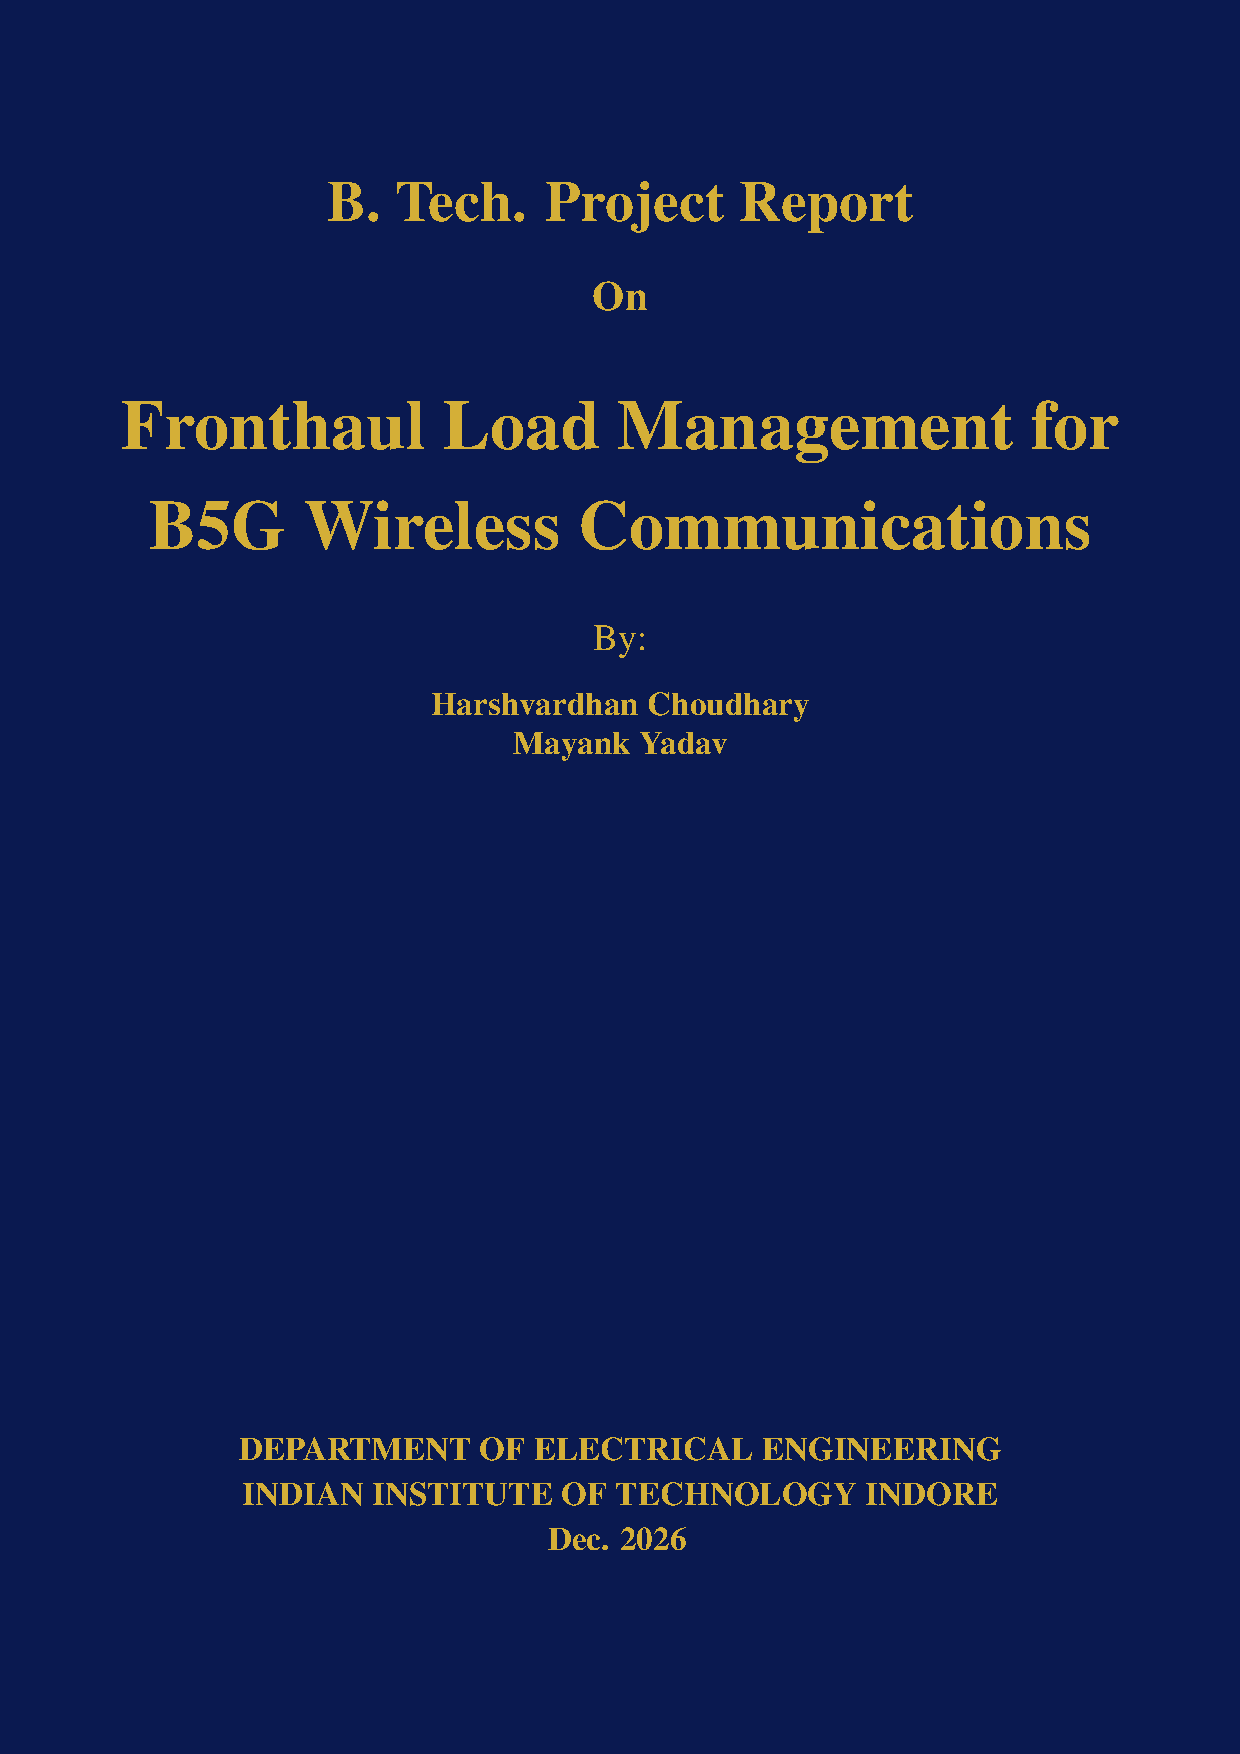
\includepdf[pages=1,pagecommand={\thispagestyle{empty}}]{BTP_hardcover.pdf}

\begin{titlepage}
\begin{center}
\vspace*{10pt}
{\Large \bf Fronthaul Load Management for\\ B5G Wireless Communications}\\[22pt]
{\large \bf A PROJECT REPORT}\\[30pt]
\emph{Submitted in partial fulfillment of the requirements\\ for the award of the degree of}\\[6pt]
{\large \bf BACHELOR OF TECHNOLOGY}\\
{\large in}\\
{\large \bf \MakeUppercase{\discipline}}\\[30pt]
Submitted by:\\[8pt]
{\large \bf \studentA} (Roll No.\ \rollA)\\
{\large \bf \studentB} (Roll No.\ \rollB)\\[18pt]
Guided by:\\[6pt]
{\large \bf \guidename}\\[30pt]

\includegraphics[scale=0.25]{IITI.png}\\[20pt]
{\Large \bf DEPARTMENT OF \MakeUppercase{\discipline}\\
INDIAN INSTITUTE OF TECHNOLOGY INDORE\\
\btpdate}
\end{center}
\end{titlepage}

\pagenumbering{roman}
\setcounter{page}{1}

% =====================================================================
\chapter*{Declaration}
\addcontentsline{toc}{chapter}{Declaration}
We hereby declare that the project entitled \textbf{``\btptitle''} submitted in partial fulfillment for the award of the degree of Bachelor of Technology in \textbf{\discipline}, completed under the supervision of \textbf{\guidename}, \guidedesig, IIT Indore, is an authentic work.

Further, we declare that we have not submitted this work for the award of any other degree elsewhere.

We declare that this written submission represents our ideas in our own words and where others' ideas or words have been included, we have adequately cited and referenced the original sources. We also declare that we have adhered to all principles of academic honesty and integrity and have not misrepresented or fabricated or falsified any idea/data/fact/source in our submission. We understand that any violation of the above will be cause for disciplinary action by the institute and can also evoke penal action from the sources which have thus not been properly cited or from whom proper permission has not been taken when needed.

\vspace{2.5cm}
\noindent
\begin{tabular}{@{}p{0.48\textwidth}p{0.48\textwidth}@{}}
\rule{5cm}{0.4pt} & \rule{5cm}{0.4pt}\\
\studentA & \studentB\\
Roll No.\ \rollA & Roll No.\ \rollB
\end{tabular}

\vspace{1.5cm}
\noindent Date: ........................\\
Place: ........................

% =====================================================================
\chapter*{Preface}
\addcontentsline{toc}{chapter}{Preface}
This report on \textbf{``\btptitle''} is prepared under the guidance of \textbf{\guidename}.

In a modern 5G network, the fronthaul is the link between the radio unit on the antenna mast and the processing unit that runs the baseband. It is the most demanding transport segment in the network. One 64-antenna cell can produce more than 15~Gbit/s of raw IQ samples, and operators usually connect many such cells through a single shared Ethernet link. This project looks at the fronthaul load problem from two sides. In Part~A we shrink the data and make the processing unit fast enough to handle it. The tools here are structure-aware IQ encoders, an adaptive functional split, a complex inversion method guided by random matrix theory and a hand-optimised C/AVX-512 precoder kernel. In Part~B we decide every 10~ms, before the traffic is known, how much of a shared link each cell may use. This part builds up from a deadline-feasible demand target and a calibrated quantile forecaster to a closed-form newsvendor allocation rule and a Bayesian Transformer forecaster. It ends with the back-pressure newsvendor controller, which outperformed the strongest known baselines in every scenario we tested.

We have tried, as far as our ability and knowledge allow, to explain the material clearly, starting from the basics of the radio access network. The report includes block diagrams of the network architecture, the algorithms and the controllers, along with the plots and tables from all experiments, so that a reader new to the field can follow it.

\vspace{2cm}
\noindent
\studentA, \studentB\\
B.Tech.\ IV Year\\
Department of \discipline\\
IIT Indore

% =====================================================================
\chapter*{B.\,Tech.\ Project Approval Certificate}
\addcontentsline{toc}{chapter}{Approval Certificate}
It is certified that the above statements made by the students are correct to the best of my knowledge and that the report titled \textbf{``\btptitle''} submitted by \textbf{\studentA} (Roll No.\ \rollA) and \textbf{\studentB} (Roll No.\ \rollB) is approved for the award of the degree of \textbf{Bachelor of Technology} in \textbf{\discipline}.

\vspace{2cm}
\begin{flushright}
Signature of BTP Guide: \hspace{0.5cm} ......................................\\[1cm]
Name: \hspace{0.5cm} \guidename\\[1cm]
Designation: \hspace{0.5cm} ......................................\\[1cm]
Date: \hspace{0.5cm} ......................................
\end{flushright}

% =====================================================================
\chapter*{Acknowledgements}
\addcontentsline{toc}{chapter}{Acknowledgements}
We are sincerely grateful to our project guide, \textbf{\guidename}, for the support, encouragement and technical direction we received over the course of this project. We were given the freedom to follow the problem from compression theory through to controller design, and the regular, critical feedback on our results shaped much of this work. We feel fortunate to have carried out our project under such generous guidance.

We thank the Department of \discipline, IIT Indore, for its computing facilities and for the chance to present this work at the mid-term and final evaluations. The questions raised by the evaluation committee there led us to adopt stronger baselines and to make our evaluation fairer.

We also thank our friends, whose support and encouragement kept our spirits up throughout. Finally, we owe special gratitude and love to our families for their unfailing support.

\vspace{2cm}
\noindent
\studentA, \studentB\\
B.Tech.\ IV Year\\
Department of \discipline\\
IIT Indore

% =====================================================================
\chapter*{Abstract}
\addcontentsline{toc}{chapter}{Abstract}
In the O-RAN 7-2x functional split, the fronthaul between the radio unit (O-RU) and the distributed unit (O-DU) carries frequency-domain IQ samples for every scheduled resource block, at rates of 7--15~Gbit/s per cell. Operators therefore compress the IQ data and connect many cells through one over-subscribed Ethernet link. This project reduces fronthaul load in two complementary ways.

Part~A makes the data smaller and the O-DU faster. O-RAN block floating point compresses the reference-symbol IQ, from which the O-DU estimates the channel, by only about 2$\times$. We propose two structure-aware encoders for it, CSEE (delay-domain sparsity) and RAS-BFP (randomised sketch and QR). In a link-level test of MMSE detection and RZF precoding, CSEE at 31$\times$ loses less than 0.05\,\% of the sum-rate, and RAS-BFP at 4$\times$ less than 0.8\,\%. Reference symbols make up 1--3 of the 14 symbols of an uplink slot, so this removes 4--20\,\% of the uplink fronthaul bits beyond BFP. For the per-slot RZF precoder, our random-matrix-guided warm-start inversion (RMT-WS) needs 6 GEMMs, while Neumann-type methods need more than 10. A fused C/AVX-512/OpenMP kernel computes the whole precoder 1.9--11$\times$ faster than a C precoder on OpenBLAS/LAPACK using the same four cores. It is the only implementation we measured that fits the 0.5~ms slot for 16 users (0.23 against 0.96~ms). This makes per-slot precoding at the radio unit possible, cutting the downlink fronthaul by 72\,\% at 99.7\,\% of the exact sum-rate.

Part~B shares one link among eight cells with 2~ms and 10~ms deadlines. We forecast the deadline-feasible rate of each cell as a set of quantiles. A closed-form KKT (constrained newsvendor) rule then splits the link so that every cell is cut at the same priority-weighted risk. Against twelve reference controllers, before the strongest baselines below were added, the KKT rule was best in all scenarios of two traffic families and beat a point forecast by 11--43\,\% on every seed. A Bayesian, link-aware Transformer forecaster improves it further, by 21\,\% at low and 6\,\% at moderate load. Two stronger baselines from the queueing and policy-search literature, predictive MaxWeight and cross-entropy policy search, outperform the KKT rule. Our final controller, the back-pressure newsvendor (BPN), is a learned policy that contains both as special cases. BPN beats both in all 10 scenarios of three traffic families by 3--25\,\% ($p \le 0.024$). On held-out sessions of a public 5G operator dataset, BPN again leads the best baseline by 6--7\,\%. An overfitting check shows that this lead does not come from tuning.

\vspace{2mm}
\noindent\textbf{\emph{Keywords}}: O-RAN, fronthaul, split 7-2x, IQ compression, matrix inversion, RZF precoding, SIMD kernels, quantile forecasting, newsvendor, Transformer, back-pressure, resource allocation.

% =====================================================================
\tableofcontents
\listoffigures
\addcontentsline{toc}{chapter}{List of Figures}
\listoftables
\addcontentsline{toc}{chapter}{List of Tables}

% =====================================================================
\chapter*{List of Abbreviations}
\addcontentsline{toc}{chapter}{List of Abbreviations}
\begin{tabbing}
xxxxxxxxxxxxxxx \= \kill
3GPP \> 3rd Generation Partnership Project\\
AVX-512 \> Advanced Vector Extensions (512-bit SIMD)\\
BBU \> Baseband Unit\\
BFP \> Block Floating Point\\
BPN \> Back-Pressure Newsvendor\\
CEM \> Cross-Entropy Method\\
CPRI / eCPRI \> (enhanced) Common Public Radio Interface\\
CSEE \> circulant / delay-domain sparse IQ encoder (proposed)\\
CU / DU / RU \> Central / Distributed / Radio Unit\\
DAgger \> Dataset Aggregation (imitation learning)\\
DF-LCQT \> Decision-Focused LCQT\\
eMBB \> enhanced Mobile Broadband\\
FiLM \> Feature-wise Linear Modulation\\
GBM \> Gradient-Boosted Machine (trees)\\
GEMM \> General Matrix--Matrix Multiplication\\
HOL \> Head of Line\\
IQ \> In-phase and Quadrature samples\\
KKT \> Karush--Kuhn--Tucker (conditions)\\
LCQT \> Link-aware Cross-cell Quantile Transformer\\
LL \> Low-Latency (traffic class)\\
LAPACK \> Linear Algebra PACKage\\
MC \> Monte Carlo\\
MDP / POMDP \> (Partially Observable) Markov Decision Process\\
MIMO \> Multiple-Input Multiple-Output\\
MMSE \> Minimum Mean-Square Error\\
MP \> Marchenko--Pastur (law)\\
NMSE \> Normalised Mean-Square Error\\
NS \> Newton--Schulz (iteration)\\
O-RAN \> Open Radio Access Network\\
OFDM \> Orthogonal Frequency-Division Multiplexing\\
PRB \> Physical Resource Block\\
RAN \> Radio Access Network\\
RAS-BFP \> randomised sketch-and-QR encoder with block floating point (proposed)\\
RIC \> RAN Intelligent Controller\\
RMT-WS \> Random-Matrix-Theory guided Warm-Start inversion\\
RZF \> Regularised Zero-Forcing (precoding)\\
SNR \> Signal-to-Noise Ratio\\
SRHT \> Subsampled Randomised Hadamard Transform\\
SVD \> Singular Value Decomposition\\
TDL \> Tapped Delay Line (channel model)\\
UE \> User Equipment\\
URLLC \> Ultra-Reliable Low-Latency Communication\\
XR \> Extended Reality
\end{tabbing}

% =====================================================================
\chapter*{Nomenclature}
\addcontentsline{toc}{chapter}{Nomenclature}
\begin{tabbing}
xxxxxxxxxxxxxx \= \kill
\textbf{Part A}\\
$Y, H, X, W$ \> received IQ matrix, channel, transmitted symbols, noise ($\mathbb{C}^{M\times N}$)\\
$M, N$ \> number of antennas, number of subcarriers\\
$K$ \> number of delay taps kept (CSEE) / number of users (precoding)\\
$r$ \> rank of the low-rank approximation\\
$b$ \> BFP mantissa width (bits)\\
$G$ \> regularised Gram matrix $HH^H + \alpha I$\\
$W_{\rm RZF}$ \> RZF precoder $H^H G^{-1}$\\
$[a,b]$ \> spectral interval of the equilibrated Gram matrix\\
$\rho,\ f_D$ \> slot-to-slot channel correlation, Doppler frequency\\[6pt]
\textbf{Part B}\\
$N$ \> number of cells sharing the link (8)\\
$C$ \> link capacity per slot (bits)\\
$T,\ \tau,\ H$ \> control interval, telemetry delay, lead time $H = T+\tau$ (slots)\\
$D_i$ \> deadline of cell $i$ (slots)\\
$w_i$ \> priority weight of cell $i$\\
$\beta(b)$ \> fronthaul bits per PRB-layer per slot\\
$d_i(t)$ \> fronthaul demand of cell $i$ in slot $t$\\
$r_i$ \> budget of cell $i$ for one interval\\
$\rstar_i$ \> deadline-feasible rate of cell $i$\\
$B_i$ \> backlog rate (queued bits / remaining slack)\\
$F_i,\ F_i^{-1}$ \> forecast distribution and quantile function of $\rstar_i$\\
$\lambda$ \> shadow price of link capacity\\
$V_w$ \> priority-weighted deadline-violation ratio\\
$\eta,\ a,\ p^0$ \> BPN sharing exponent, drain-rate mix, class base quantile
\end{tabbing}

% =====================================================================
\cleardoublepage
\pagenumbering{arabic}
\setcounter{page}{1}

% =====================================================================
\chapter{Introduction}
\thispagestyle{plain}
% =====================================================================

\section{Introduction}

Whenever a mobile phone places a call, plays a video or runs an app, its traffic reaches the Internet through a \emph{radio access network} (RAN). The RAN turns the radio signal at the antenna into packets, and packets back into radio signals. It also schedules thousands of users on shared spectrum every half millisecond. Over three generations the RAN has changed shape. It started as a single cabinet at the foot of each tower and has become a chain of specialised units joined by packet networks. How many cells an operator can deploy, and at what cost, now depends on the rate, latency and reliability of the links in this chain, and most of all on the first one, the \emph{fronthaul}. This project deals with managing the load on that link.

\subsection{The mobile transport network: fronthaul, midhaul and backhaul}

Figure~\ref{fig:transport} traces a user's data through a 5G network. On the mast sits the radio unit (RU). It contains the antennas and the radio-frequency chain, and in the O-RAN split it also takes the lower part of the physical layer. The distributed unit (DU) handles the time-critical baseband, which means the rest of the physical layer, the MAC scheduler and RLC. Higher protocols with looser timing (PDCP, RRC, SDAP) run in the central unit (CU), and one CU can serve many DUs. Mobility, sessions and the connection to the Internet are left to the 5G core.

The requirements on the three transport segments between these units differ a great deal.
\begin{itemize}
  \item \textbf{Fronthaul} (RU $\leftrightarrow$ DU) is the hardest of the three. It carries digitised radio samples (IQ samples) at tens of Gbit/s per cell, with a one-way latency budget of about 100~$\mu$s. A packet that arrives late is of no use to the radio.
  \item \textbf{Midhaul} (DU $\leftrightarrow$ CU) sees packet data that has already passed the MAC/RLC layers. Its rate is close to the user data rate and it can tolerate a few milliseconds of latency.
  \item \textbf{Backhaul} (CU $\leftrightarrow$ core) brings the combined user traffic of many cells to the core network, where latencies of about 10~ms or more are acceptable.
\end{itemize}

\begin{figure}[H]
\centering
\begin{tikzpicture}[font=\small,>=Stealth,
  unit/.style={draw,rounded corners,align=center,minimum height=1.25cm,minimum width=1.75cm,inner sep=3pt},
  lbl/.style={font=\footnotesize\bfseries,align=center}]
  % UE
  \node[unit,fill=gray!12,minimum width=1.2cm] (ue) at (0,0) {UE\\[-1pt]\scriptsize phones};
  % tower
  \begin{scope}[shift={(2.25,-0.62)}]
    \draw[thick] (0,0) -- (0.32,1.55) -- (0.64,0);
    \draw (0.08,0.4) -- (0.56,0.4); \draw (0.16,0.8) -- (0.48,0.8); \draw (0.24,1.2) -- (0.40,1.2);
    \draw[fill=iitblue!35] (0.22,1.55) rectangle (0.42,1.95);
    \draw[iitblue] (0.52,1.85) arc (-30:30:0.25); \draw[iitblue] (0.62,1.85) arc (-30:30:0.38);
  \end{scope}
  \node[unit,fill=iitblue!15] (ru) at (4.0,0) {O-RU\\[-1pt]\scriptsize RF + low PHY};
  \node[unit,fill=good!15] (du) at (7.3,0) {O-DU\\[-1pt]\scriptsize high PHY,\\[-4pt]\scriptsize MAC, RLC};
  \node[unit,fill=orange!18] (cu) at (10.2,0) {O-CU\\[-1pt]\scriptsize PDCP, RRC};
  \node[unit,fill=purple!12] (core) at (13.0,0) {5G Core\\[-1pt]\scriptsize + Internet};
  \draw[<->,dashed,thick] (ue) -- (2.35,0);
  \node[font=\scriptsize] at (1.2,0.35) {air};
  \draw[<->,line width=2.6pt,accent] (ru) -- (du);
  \draw[<->,line width=1.6pt,orange!80!black] (du) -- (cu);
  \draw[<->,line width=1.0pt,purple!70!black] (cu) -- (core);
  \node[lbl,text=accent] at (5.65,1.2) {FRONTHAUL};
  \node[lbl,text=orange!80!black] at (8.75,1.2) {MIDHAUL};
  \node[lbl,text=purple!70!black] at (11.6,1.2) {BACKHAUL};
  \node[font=\scriptsize,align=center,text=accent] at (5.65,-1.45) {IQ samples\\7--100+ Gbit/s\\$\approx$100\,$\mu$s};
  \node[font=\scriptsize,align=center,text=orange!80!black] at (8.75,-1.45) {packets\\$\approx$ user rate\\$\approx$1--5\,ms};
  \node[font=\scriptsize,align=center,text=purple!70!black] at (11.6,-1.45) {aggregated\\traffic\\$\approx$10\,ms};
  \draw[decorate,decoration={brace,amplitude=6pt,mirror},thick] (3.1,-2.25) -- (14.0,-2.25)
     node[midway,below=8pt,font=\footnotesize] {Mobile transport network (``X-haul'')};
\end{tikzpicture}
\caption{End-to-end path of user data in a disaggregated 5G RAN, with the three transport segments and their typical rates and latency budgets. The fronthaul, highlighted, is the subject of this project.}
\label{fig:transport}
\end{figure}

\subsection{From distributed RAN to Open RAN}

A classical \emph{distributed RAN} (D-RAN) keeps the whole baseband unit (BBU) in a cabinet at each site, so only backhaul leaves the site. \emph{Centralised RAN} (C-RAN) pulled the BBUs of many sites into a central pool, where they could share hardware and coordinate cells. The cost of this was a fronthaul link carrying raw radio samples over the CPRI protocol. Its rate is constant and proportional to bandwidth $\times$ antennas, and it stays the same whether or not anyone is using the cell. Once radios have 64 antennas for massive MIMO and carriers are 100~MHz wide, CPRI would need hundreds of Gbit/s per cell, which is not practical. So 5G split the baseband in a new place (Figure~\ref{fig:evolution}). Part of the physical layer went back into the radio unit. The fronthaul now uses packet-based eCPRI on ordinary Ethernet and carries frequency-domain samples only for the resource blocks that are actually scheduled.

\begin{figure}[H]
\centering
\begin{tikzpicture}[font=\footnotesize,>=Stealth,
  b/.style={draw,rounded corners,align=center,minimum height=0.75cm,inner sep=2pt},
  row/.style={font=\footnotesize\bfseries,anchor=east,align=right}]
  % D-RAN
  \node[row] at (-0.3,0) {D-RAN};
  \node[b,fill=iitblue!15,minimum width=1.0cm] (r1) at (0.6,0) {RRH};
  \node[b,fill=good!15,minimum width=1.6cm] (b1) at (2.5,0) {BBU (at site)};
  \node[b,fill=purple!12,minimum width=1.4cm] (c1) at (9.5,0) {Core};
  \draw[<->,thick] (r1) -- (b1);
  \draw[<->,thick,purple!70!black] (b1) -- node[above]{backhaul} (c1);
  % C-RAN
  \node[row] at (-0.3,-1.6) {C-RAN};
  \node[b,fill=iitblue!15,minimum width=1.0cm] (r2) at (0.6,-1.6) {RRH};
  \node[b,fill=good!15,minimum width=1.9cm] (b2) at (5.0,-1.6) {BBU pool};
  \node[b,fill=purple!12,minimum width=1.4cm] (c2) at (9.5,-1.6) {Core};
  \draw[<->,line width=2.4pt,accent] (r2) -- node[above=2pt,text=accent]{CPRI: constant, huge} (b2);
  \draw[<->,thick,purple!70!black] (b2) -- node[above]{backhaul} (c2);
  % O-RAN
  \node[row] at (-0.3,-3.2) {O-RAN};
  \node[b,fill=iitblue!15,minimum width=1.0cm] (r3) at (0.6,-3.2) {O-RU};
  \node[b,fill=good!15,minimum width=1.2cm] (d3) at (4.0,-3.2) {O-DU};
  \node[b,fill=orange!18,minimum width=1.2cm] (u3) at (6.6,-3.2) {O-CU};
  \node[b,fill=purple!12,minimum width=1.4cm] (c3) at (9.5,-3.2) {Core};
  \draw[<->,line width=1.6pt,accent] (r3) -- node[above=2pt,text=accent]{eCPRI 7-2x} node[below=2pt,text=accent,font=\scriptsize]{load-dependent} (d3);
  \draw[<->,thick,orange!80!black] (d3) -- node[above]{midhaul} (u3);
  \draw[<->,thick,purple!70!black] (u3) -- node[above]{backhaul} (c3);
\end{tikzpicture}
\caption{Evolution of the RAN architecture. In C-RAN the CPRI fronthaul has a constant, very high rate; in O-RAN split 7-2x it carries only scheduled resource blocks, so the load follows the traffic and can be statistically multiplexed.}
\label{fig:evolution}
\end{figure}

\subsection{Functional splits and the O-RAN 7-2x split}

3GPP TR 38.801 lists eight points where the protocol stack can be cut between a central and a remote unit (Figure~\ref{fig:splits}). A high split such as Option 2 gives a lower transport rate that follows the traffic, but it leaves the central unit less room to coordinate. A low split such as Option 8 (CPRI) centralises more. The price is a transport rate that is huge and constant. For Open RAN, the O-RAN Alliance chose the intra-PHY split 7-2x as the fronthaul. The O-RU keeps the FFT, cyclic-prefix handling and, optionally, precoding. Channel estimation, equalisation, decoding and scheduling run in the O-DU. What crosses the fronthaul is frequency-domain IQ samples for every scheduled physical resource block (PRB) and every MIMO layer, compressed with \emph{block floating point} (BFP).

\begin{figure}[H]
\centering
\begin{tikzpicture}[font=\footnotesize,>=Stealth,
  layer/.style={draw,fill=soft,minimum width=2.1cm,minimum height=0.6cm,align=center},
  cut/.style={draw=accent,thick,dashed}]
  \node[layer] (rrc)  at (0,0)    {RRC};
  \node[layer] (pdcp) at (0,-0.6) {PDCP};
  \node[layer] (rlch) at (0,-1.2) {High RLC};
  \node[layer] (rlcl) at (0,-1.8) {Low RLC};
  \node[layer] (mach) at (0,-2.4) {High MAC};
  \node[layer] (macl) at (0,-3.0) {Low MAC};
  \node[layer] (phyh) at (0,-3.6) {High PHY};
  \node[layer] (phyl) at (0,-4.2) {Low PHY};
  \node[layer] (rf)   at (0,-4.8) {RF};
  \foreach \y/\o in {-0.3/1,-0.9/2,-1.5/3,-2.1/4,-2.7/5,-3.3/6,-3.9/7,-4.5/8}{
     \draw[cut] (-1.25,\y) -- (1.25,\y);
     \node[anchor=west,text=accent] at (1.3,\y) {Option \o};
  }
  \draw[line width=1.4pt,good] (-1.35,-3.9) -- (1.35,-3.9);
  \node[anchor=west,text=good,font=\footnotesize\bfseries] at (2.6,-3.9) {$\leftarrow$ O-RAN split 7-2x};
  \draw[->,thick] (-2.0,-0.1) -- (-2.0,-4.7);
  \node[rotate=90,font=\scriptsize,align=center] at (-2.5,-2.4) {lower split $\Rightarrow$ more centralisation,\\higher and less elastic fronthaul rate};
  \node[anchor=west,font=\scriptsize,align=left] at (6.1,-1.2) {\textbf{Option 2} (CU/DU, F1):\\packet rate $\approx$ user rate};
  \node[anchor=west,font=\scriptsize,align=left] at (6.1,-2.5) {\textbf{Option 7-2x} (DU/RU):\\frequency-domain IQ per scheduled PRB,\\BFP compressed, eCPRI over Ethernet};
  \node[anchor=west,font=\scriptsize,align=left] at (6.1,-4.4) {\textbf{Option 8} (CPRI):\\time-domain samples, constant rate};
\end{tikzpicture}
\caption{Functional split options of 3GPP TR 38.801 on the RAN protocol stack. The O-RAN fronthaul uses the intra-PHY split 7-2x.}
\label{fig:splits}
\end{figure}

\subsection{The O-RAN architecture}

O-RAN does more than open the fronthaul. It also adds two programmable controllers (Figure~\ref{fig:oran}). The non-real-time RIC lives inside the service management and orchestration (SMO) framework, where it trains models and runs ``rApps'' on time scales above one second. The near-real-time RIC runs ``xApps'', which control the O-CU and O-DU over the E2 interface in a 10~ms--1~s loop. A fronthaul budget controller like the one we build in Part~B fits here naturally. It can be deployed as an xApp or as a function inside the O-DU pool, and it works at the 10~ms time scale of the near-RT RIC.

\begin{figure}[H]
\centering
\begin{tikzpicture}[font=\footnotesize,>=Stealth,
  b/.style={draw,rounded corners,align=center,minimum height=0.85cm,inner sep=3pt}]
  \node[b,fill=purple!10,minimum width=10.5cm,minimum height=1.0cm] (smo) at (3.5,3.6) {Service Management and Orchestration (SMO)\quad $\supset$\quad \textbf{Non-RT RIC} (rApps, $>1$\,s)};
  \node[b,fill=orange!12,minimum width=7.6cm] (ric) at (3.5,2.1) {\textbf{Near-RT RIC} (xApps, 10\,ms -- 1\,s)\ \ e.g.\ \emph{fronthaul budget xApp}};
  \node[b,fill=orange!18,minimum width=2.0cm] (cu) at (0.6,0.4) {O-CU};
  \node[b,fill=good!15,minimum width=2.0cm] (du) at (3.5,0.4) {O-DU};
  \node[b,fill=iitblue!15,minimum width=2.0cm] (ru) at (7.3,0.4) {O-RU};
  \draw[<->,thick] (smo.south -| ric.north) -- node[right]{A1} (ric.north);
  \draw[<->,thick] (ric.south -| cu.north) -- node[left]{E2} (cu.north);
  \draw[<->,thick] (ric.south -| du.north) -- node[left]{E2} (du.north);
  \draw[<->,thick] (cu) -- node[above]{F1} (du);
  \draw[<->,line width=2.2pt,accent] (du) -- node[above,text=accent,font=\footnotesize\bfseries]{Open FH} node[below,text=accent,font=\scriptsize]{7-2x} (ru);
  \draw[<->,thick,dashed] (smo.east) -- ++(0.6,0) |- node[pos=0.75,above]{O1 / O2} (ru.east);
\end{tikzpicture}
\caption{O-RAN architecture with its open interfaces. The open fronthaul (7-2x) connects O-DU and O-RU; the near-RT RIC controls the RAN over E2 at the 10~ms time scale used by our Part~B controller.}
\label{fig:oran}
\end{figure}

\subsection{Why the fronthaul is loaded}

In a 7-2x cell, the fronthaul load depends on how many PRB-layers are scheduled. The number of user bits does not set it. For one PRB on one layer in one slot, the O-RAN BFP format sends 12 subcarriers $\times$ 14 symbols of $b$-bit I and Q mantissas, plus an exponent. With a 9-bit mantissa that comes to about 3{,}400 bits. At its peak, a 100~MHz carrier with 273 PRBs and 4 layers needs about 7.4~Gbit/s. A 64-antenna receiver that forwards every antenna stream needs about 15.4~Gbit/s, and DU-side precoding for 64 streams needs more than 118~Gbit/s. Cells rarely peak at the same moment. Operators use this by connecting many cells through one aggregation switch and one 25 or 100~Gbit Ethernet link, with a capacity well below the sum of the peaks (Figure~\ref{fig:shared}). Such \emph{statistical multiplexing} keeps Open RAN fronthaul affordable. But it also means the link fails when bursts happen together.

\begin{figure}[H]
\centering
\begin{tikzpicture}[font=\footnotesize,>=Stealth,
   ru/.style={draw,fill=iitblue!15,rounded corners,minimum width=1.7cm,minimum height=0.55cm,align=center},
   ll/.style={draw,fill=accent!15,rounded corners,minimum width=1.7cm,minimum height=0.55cm,align=center}]
  \node[ll] (r1) at (0,3.0) {O-RU 1 (LL)};
  \node[ll] (r2) at (0,2.3) {O-RU 2 (LL)};
  \node[ll] (r3) at (0,1.6) {O-RU 3 (LL)};
  \node[ru] (r4) at (0,0.9) {O-RU 4 (eMBB)};
  \node at (0,0.35) {$\vdots$};
  \node[ru] (r8) at (0,-0.3) {O-RU 8 (eMBB)};
  \node[draw,fill=gray!20,circle,minimum size=1.1cm,align=center] (sw) at (3.4,1.35) {switch};
  \node[draw,fill=good!15,rounded corners,minimum width=2.4cm,minimum height=1.4cm,align=center] (du) at (9.3,1.35) {O-DU pool\\\scriptsize + budget controller};
  \foreach \r in {r1,r2,r3,r4,r8} \draw[<->] (\r.east) -- (sw);
  \draw[<->,line width=3pt,accent] (sw) -- (du);
  \node[text=accent,align=center] at (6.1,1.95) {\textbf{one shared 25GE link}};
  \node[text=accent,align=center,font=\scriptsize] at (6.1,0.75) {$\sum$ cell peaks $= 2.44\times$ capacity};
  \node[align=left,font=\scriptsize,anchor=west] at (-1.0,-1.15) {LL: 2\,ms deadline, priority 3 \qquad eMBB: 10\,ms deadline, priority 1};
\end{tikzpicture}
\caption{Shared fronthaul scenario of Part~B: eight 7-2x cells with different deadlines share one over-subscribed Ethernet link through an aggregation switch.}
\label{fig:shared}
\end{figure}

\section{Motivation for BTP and Problem Statement}

Two bottlenecks limit how cheaply, and how densely, Open RAN cells can be deployed.
\begin{enumerate}
  \item \textbf{The data are large and the processing time is short.} O-RAN BFP compression does little more than shorten the numbers, and it gets about 2$\times$ over 16-bit I/Q. On top of that, the O-DU has to compute a precoder for all 273 PRBs in every 0.5~ms slot. Each PRB needs the inverse of a complex $K\times K$ Gram matrix. With a standard numpy + LAPACK implementation and 16 users this takes 3.2~ms, more than six times the slot length.
  \item \textbf{The link is shared and smaller than the peak.} If several cells burst at once, the shared link cannot carry all of it, and low-latency (LL) cells can wait only about 2~ms. Some coordinator has to decide beforehand how many bits each cell may send. It makes this decision every 10~ms using telemetry that is already 1~ms old, and it cannot see the next burst. Any cell that gets too small a share loses data.
\end{enumerate}

We tackle both bottlenecks with the same guiding principle: \emph{keep the mathematical structure of the problem, and learn only what is uncertain}.

\paragraph{Problem statement (Part A).} The first aim is IQ compression with error bounds that uses the low rank and delay-domain sparsity of the received signal to go well past the 2$\times$ of BFP. The second is a per-slot complex precoder that is fast and accurate enough to run inside the 0.5~ms slot on a general-purpose CPU.

\paragraph{Problem statement (Part B).} Suppose we have a forecast of each cell's fronthaul need over the next interval. We want a controller that sets per-cell budgets on a shared 7-2x link every 10~ms, before the traffic is seen, and that minimises the priority-weighted fraction of bits missing their deadline. We also want to show that it beats the strongest available controllers when all of them run on identical traffic and are compared with paired statistics.

\section{Objectives and Contributions}

\begin{figure}[H]
\centering
\begin{tikzpicture}[font=\footnotesize,>=Stealth,
   lever/.style={draw,rounded corners,align=left,text width=6.6cm,inner sep=6pt}]
  \node[lever,fill=iitblue!8] (A) at (0,0) {%
    \textbf{\textcolor{iitblue}{Part A: make the data smaller and the DU faster}}\\[3pt]
    $\bullet$ CSEE and RAS-BFP structure-aware IQ encoders\\
    $\bullet$ 8-method inversion benchmark, learned InverseNets\\
    $\bullet$ RMT-WS warm-start complex inversion\\
    $\bullet$ Fused C/AVX-512/OpenMP RZF precoder kernel\\
    $\bullet$ RU-side precoding: $-72\,\%$ downlink fronthaul};
  \node[lever,fill=accent!6] (B) at (7.4,0) {%
    \textbf{\textcolor{accent}{Part B: share one link well}}\\[3pt]
    $\bullet$ Deadline-feasible rate $\rstar$ as the demand target\\
    $\bullet$ B1: GBM quantiles + closed-form KKT rule\\
    $\bullet$ Theory: MDP view, Markov-fluid bounds on $\rstar$\\
    $\bullet$ B2: Bayesian link-aware Transformer (LCQT)\\
    $\bullet$ B3: back-pressure newsvendor (BPN)\\
    $\bullet$ 3 traffic families, 19+ controllers, paired tests};
  \node[draw,rounded corners,fill=good!12,text width=14cm,align=center,inner sep=5pt,anchor=north] (AB) at ($(B.south)+(-3.7,-0.7)$) {%
    Part A $\times$ Part B: the compression width sets \emph{how much} load reaches the link;
    the allocation rule decides \emph{who} loses data when bursts coincide.};
  \draw[->,thick] (A.south) -- (A.south |- AB.north);
  \draw[->,thick] (B.south) -- (B.south |- AB.north);
\end{tikzpicture}
\caption{The two levers of fronthaul load management developed in this project and how they combine.}
\label{fig:overview}
\end{figure}

This project makes the following contributions.
\begin{enumerate}
  \item \textbf{Structure-aware IQ compression.} We propose two encoders with error bounds for the reference-symbol IQ used in channel estimation. CSEE exploits delay-domain sparsity at $O(MN\log N)$ cost, and RAS-BFP uses a randomised SRHT sketch and QR at $O(rMN)$. In link-level checks, CSEE loses less than 0.05\,\% of the sum-rate at 31$\times$ and RAS-BFP less than 0.8\,\% at 4$\times$, where O-RAN BFP reaches about 2$\times$. At 64 antennas both encode faster than truncated SVD. Used on the reference symbols of each uplink slot, they save 4--20\,\% of the uplink fronthaul bits beyond what BFP gives.
  \item \textbf{Fast complex inversion for the precoder.} We screen 8 methods on CPU, including two learned Newton--Schulz inverters. We also develop RMT-WS, a Chebyshev/Newton--Schulz inversion guided by random-matrix theory. It tracks a warm start, follows a Doppler law and returns a residual certificate, and it needs 6 GEMMs where Neumann-type schemes need more than 10.
  \item \textbf{Kernel engineering.} Our fused C/AVX-512/OpenMP RZF precoder is 1.6--3.9$\times$ faster than a C precoder on OpenBLAS/LAPACK on one core, and 1.9--11$\times$ faster on four. Of the implementations we measured, it alone fits the whole precoder for 16 users into the 0.5~ms slot. That makes per-slot RU-side precoding possible, and with it the downlink fronthaul rate drops by 72\,\% while keeping 99.7\,\% of the exact sum-rate.
  \item \textbf{The KKT newsvendor rule (B1).} The rule forecasts the deadline-feasible rate $\rstar$ as a range and splits the link so that every cell carries equal priority-weighted risk. We prove four properties of it. In the NCC comparison it was the best of the 12 reference controllers in all scenarios of two traffic families (submitted to NCC 2027). Stronger baselines that we added later do beat it, and this is what led to B3.
  \item \textbf{Theory and stronger baselines.} We write the problem as a POMDP and derive Markov-fluid bounds linking $\rstar$ to effective bandwidth. We also add a third traffic family and the strongest baselines we could implement, namely predictive MaxWeight and cross-entropy policy search.
  \item \textbf{A Bayesian, link-aware Transformer forecaster (B2).} LCQT uses deadline-aware patch tokens with FiLM conditioning and cross-cell attention. Its outputs are non-crossing quantiles, and it ends in a Bayesian mixture layer followed by a differentiable KKT layer.
  \item \textbf{The back-pressure newsvendor (B3).} This is a two-stage policy class that includes both strongest baselines as exact special cases. Learned with the same search effort, it beats them in all 10 scenarios of three traffic families by 3--25\,\%. On held-out real 5G traces the margin is 6--7\,\%.
\end{enumerate}

\section{Organization of the Report}

Chapter~\ref{ch:lit} surveys prior work on fronthaul transport, IQ compression, massive-MIMO matrix inversion, predictive capacity allocation, uncertainty quantification and back-pressure control, and points out the gaps that this project addresses. The system model and methods of Part~A are given in Chapter~\ref{ch:parta-methods}, with their simulation results in Chapter~\ref{ch:parta-results}. Chapter~\ref{ch:partb-methods} covers Part~B. It sets up the system model and the deadline-feasible rate, and then develops the KKT newsvendor rule, the Bayesian Transformer forecaster and the back-pressure newsvendor. Their closed-loop simulation results on three traffic families appear in Chapter~\ref{ch:partb-results}. In Chapter~\ref{ch:impl} we describe the implementation and the software framework, along with the optimised CPU kernels and how they perform on real hardware. Chapter~\ref{ch:concl} concludes the report and outlines future work. Proofs, simulation parameters and instructions for reproducing the results are collected in the appendices.

% =====================================================================
\chapter{Literature Review}
\label{ch:lit}
\thispagestyle{plain}
% =====================================================================

\section{Introduction}

This chapter reviews the work on which the project builds and positions our contributions against it. Section~\ref{sec:lit-fh} covers the fronthaul itself: functional splits, the O-RAN 7-2x interface, dimensioning and statistical multiplexing of shared links. Section~\ref{sec:lit-comp} covers fronthaul compression and adaptive splits (Part~A), and Section~\ref{sec:lit-inv} fast matrix inversion and precoding for massive MIMO (Part~A). Sections~\ref{sec:lit-alloc}--\ref{sec:lit-bp} cover the literature relevant to Part~B: anticipatory capacity allocation from forecasts, uncertainty-aware forecasting and conformal allocation, the newsvendor problem and network calculus, back-pressure and policy-search control, and Transformer forecasters with decision-focused learning. Section~\ref{sec:lit-pos} compares our methods with the closest work property by property and states what is new, and Section~\ref{sec:lit-gap} summarises the research gaps.

\section{The Fronthaul: Functional Splits, O-RAN 7-2x and Shared Links}
\label{sec:lit-fh}

\paragraph{Functional splits.} 3GPP TR 38.801~\cite{tr38801} defines functional split options 1 to 8 between a central and a distributed unit. Larsen, Checko and Christiansen~\cite{larsen2019} survey the splits for 5G crosshaul and show that for splits 1 to 7-2 ``the bitrate will vary with the user load'', while only splits 7-1 and 8 are constant-rate; Ethernet transport of split 7-2 adds about 8\,\% overhead. Fronthaul demand is therefore a function of scheduled PRB-layers rather than of application bits. Both parts of this project rest on this fact.

\paragraph{O-RAN 7-2x.} The O-RAN WG4 control, user and synchronisation plane specification~\cite{oran_cus} defines the 7-2x split, section-based U-plane messages that carry IQ only for scheduled PRBs, block floating point (BFP) compression with a shared exponent per PRB and a configurable mantissa width, and receive windows at the O-RU after which U-plane packets are discarded. Polese \emph{et al.}~\cite{polese2023} give a comprehensive overview of the O-RAN architecture, its RICs and interfaces. IEEE 802.1CM~\cite{ieee8021cm} specifies time-sensitive networking profiles for fronthaul with a 100~$\mu$s one-way latency budget.

\paragraph{Dimensioning and statistical multiplexing.} P\'erez, Hern\'andez and Larrabeiti~\cite{perez2018} model packet-switched aggregation of eCPRI flows and dimension the fronthaul by high delay percentiles. Wang and Zhou~\cite{wang2017} derive the blocking probability when several radio units share one fronthaul link and show that the multiplexing gain grows with the cluster size (27.5\,\% for five units at 5\,\% blocking). Lag\'en \emph{et al.}~\cite{lagen2022} study several 7-2x cells that share one fixed-capacity link through an L2 switch and propose fronthaul-aware modulation compression and scheduling. Their control is reactive and per slot; it uses no forecasting, no uncertainty and no cross-cell deadline weighting. Koulougli \emph{et al.}~\cite{flexe2023} carry eCPRI over FlexEthernet. These works establish the shared, over-subscribed link model that we adopt in Part~B.

\section{Fronthaul Compression and Adaptive Splits}
\label{sec:lit-comp}

The O-RAN baseline is BFP~\cite{oran_cus}, which compresses each PRB to a common exponent and $b$-bit mantissas; it exploits only the dynamic range of the samples and reaches about 2$\times$ over 16-bit I/Q. Low-rank compression is grounded in the Eckart--Young theorem~\cite{eckart1936}: the truncated SVD gives the best rank-$r$ approximation in Frobenius norm, but at a cost of $O(MN\min(M,N))$ that is too high for a 0.5~ms slot. Halko, Martinsson and Tropp~\cite{halko2011} showed that a randomised sketch followed by a QR factorisation achieves a $(1+\varepsilon)$-optimal rank-$r$ factorisation at $O(rMN)$ cost; this is the theory behind our RAS-BFP encoder. The 3GPP TDL channel models of TR 38.901~\cite{tr38901} have a few strong delay taps, so the channel, and hence the de-rotated reference-symbol IQ, is sparse in the delay domain after an inverse FFT across subcarriers; our CSEE encoder exploits this structure.

\paragraph{Compression for split 8 and C-RAN.} Before O-RAN, fronthaul compression targeted the time-domain samples of split 8 (CPRI). Guo \emph{et al.}~\cite{guo2013} and Nieman and Evans~\cite{nieman2013} combine sample-rate reduction, block scaling and non-uniform quantisation of LTE time-domain samples and reach about 3$\times$ at an EVM acceptable for 64-QAM. Park \emph{et al.}~\cite{park2014} survey information-theoretic C-RAN compression (point-to-point, distributed Wyner--Ziv and multivariate compression), which is optimal in principle but needs joint statistics of all radio units and iterative design at the central unit. Checko \emph{et al.}~\cite{checko2015} review C-RAN and identify fronthaul bit rate as its main obstacle. All of these compress \emph{per antenna stream} and do not use the structure across antennas and subcarriers that a massive-MIMO 7-2x frame has.

\paragraph{Learned and sparsity-based channel compression.} CsiNet~\cite{wen2018} compresses massive-MIMO channel matrices with a convolutional autoencoder in the angular-delay domain. It targets UE-to-gNB CSI feedback, needs training for each channel scenario and a neural network at both ends, and gives no error guarantee. Sparse channel estimation by compressive sensing~\cite{berger2010} uses the same delay-domain sparsity as CSEE, but to \emph{estimate} the channel, not to code it for transport. CSEE moves this idea into the RU as a transport code with a closed-form error bound and no training; RAS-BFP does the same for the low-rank structure with the randomised range finder.

\section{Matrix Inversion and Precoding for Massive MIMO}
\label{sec:lit-inv}

Massive MIMO~\cite{marzetta2010,rusek2013} serves many users on the same PRB with tens to hundreds of antennas, and with many more antennas than users simple linear processing is close to optimal. Linear MMSE detection and regularised zero-forcing (RZF) precoding require the inverse of a $K\times K$ Gram matrix $G = HH^H + \alpha I$ for every PRB in every slot. To avoid the cubic cost of exact inversion, Wu \emph{et al.}~\cite{wu2013} and Prabhu \emph{et al.}~\cite{prabhu2013} proposed truncated Neumann series, which converge when $G$ is diagonally dominant (many more antennas than users). Shao \emph{et al.}~\cite{shao2016} combined Newton iteration with a Neumann initialisation. The classical Newton--Schulz iteration $X \leftarrow X(2I - GX)$~\cite{schulz1933,benisrael1966,pan1991} converges quadratically once the initial residual is below one, and uses only matrix multiplications, which makes it attractive for GPU and tensor-core hardware~\cite{higham2008}. Kammoun \emph{et al.}~\cite{kammoun2014} designed truncated polynomial expansion precoders using random-matrix theory. The Marchenko--Pastur law~\cite{marchenko1967} describes the limiting eigenvalue distribution of Gram matrices of i.i.d.\ channels and has been used to choose polynomial intervals; Couillet and Debbah~\cite{couillet2011} develop the random-matrix tools for wireless systems on which such designs rest. These designs fix the interval from the i.i.d.\ law, so they lose accuracy when the channel is correlated or users have very different path losses.

\paragraph{Software baseband on CPUs.} BigStation~\cite{yang2013bigstation} showed that large MU-MIMO baseband processing can run in real time on commodity servers by parallelising across many machines. Agora~\cite{ding2020agora} runs massive-MIMO baseband processing in software on one many-core server with SIMD kernels and an optimised math library, and processes each subcarrier group with standard library calls. These systems establish that a CPU O-DU is practical. They compute each precoder from scratch with library routines; our kernel instead fuses the Gram matrix, the inverse and the weights per PRB in L1 cache and reuses the previous slot's inverse. Table~\ref{tab:hw-strong} compares it against exactly such a per-PRB library baseline. Learned iterative solvers that ``unroll'' a classical iteration and learn its coefficients are an emerging line of work; we build two such inverters (InverseNet-NS and InverseNet-Ultra) and a direct regression baseline.

Our RMT-WS method combines three ideas in one per-slot inverter: an eigensolve-free spectral interval from a moment-matched Marchenko--Pastur law that also holds for correlated, near-far and line-of-sight channels; a Chebyshev polynomial initialisation followed by Newton--Schulz; and slot-to-slot warm-start tracking governed by a closed-form Doppler law and a probabilistic residual certificate.

\section{Anticipatory Capacity Allocation from Forecasts}
\label{sec:lit-alloc}

Bega \emph{et al.} proposed DeepCog~\cite{bega2019}, which forecasts the capacity needed per network slice with a deep network trained on a cost-aware loss, and AZTEC~\cite{bega2020}, a two-timescale allocation of dedicated and shared capacity from forecasts. Sciancalepore \emph{et al.}~\cite{sciancalepore2017} use traffic forecasts for slice admission. Kavehmadavani \emph{et al.}~\cite{kavehmadavani2023} feed LSTM traffic forecasts into an O-RAN traffic-steering problem with a fronthaul capacity constraint. Recent O-RAN works allocate slice resources with deep reinforcement learning xApps~\cite{dai2025,sever2025,dora2025,cheng2023}. All of these use \emph{point} forecasts (or a network trained for one fixed cost ratio), allocate at time scales of seconds to minutes, and have no notion of per-cell deadline feasibility or queue state. Predictive dynamic bandwidth allocation for PON-based fronthaul~\cite{mikaeil2018} has the same ``decide before observing'' structure, again with point predictions.

\paragraph{vRAN orchestration and O-RAN intelligence.} FluidRAN~\cite{garcia2018fluidran} chooses the functional split and the placement of vRAN functions jointly with routing, under fronthaul and backhaul capacity limits, by solving a mixed-integer program for a known, average load. vrAIn~\cite{ayala2019vrain} learns how to share computing and radio resources among virtualised base stations. Bonati \emph{et al.}~\cite{bonati2021} describe how learned control loops run as xApps and rApps in the O-RAN RICs. These works decide on time scales of seconds to hours and treat the load as known or average. Our controllers run at the 10~ms time scale of the near-real-time RIC and decide under explicit uncertainty about the next interval's demand.

\paragraph{Public traffic data.} Most allocation studies use synthetic traffic or private operator traces. Public datasets include city-scale aggregate activity, such as the Milan and Trentino data of Barlacchi \emph{et al.}~\cite{barlacchi2015}, and per-user 5G throughput and channel traces, such as the dataset of Raca \emph{et al.}~\cite{raca2020beyond}. We use the latter for a trace-driven test of Part~B (Section~\ref{sec:rb-real}).

\section{Uncertainty-Aware Forecasting and Conformal Allocation}
\label{sec:lit-unc}

Kasuluru \emph{et al.}~\cite{kasuluru2024} forecast the distribution of PRB load with DeepAR and Transformer models and study the over- and under-provisioning caused by choosing a percentile; the percentile is chosen globally rather than derived from a coupled allocation. Cohen \emph{et al.}~\cite{cohen2023} use online conformal prediction to set the amount of pre-allocated URLLC resources for a single traffic stream so that a reliability target holds. Gibbs and Cand\`es~\cite{gibbs2021} introduced adaptive conformal inference (ACI) under distribution shift, the update rule we use as a calibration ablation. Deep ensembles~\cite{lakshminarayanan2017} and Monte-Carlo dropout~\cite{gal2016} are the standard ways to represent epistemic uncertainty in deep forecasters. None of these works couples several cells through a shared capacity constraint.

\section{Newsvendor Problems, Network Calculus and Effective Bandwidth}
\label{sec:lit-nv}

The newsvendor problem goes back to the optimal inventory policy of Arrow, Harris and Marschak~\cite{arrow1951}: when the demand is uncertain and over- and under-provisioning have different costs, the optimal order is a quantile of the demand distribution. The multi-item newsvendor with a budget constraint~\cite{hadley1963} has a classical solution: at the optimum, the marginal expected value of one more unit is equal across items, which yields a quantile of each item's demand distribution set by a common Lagrange multiplier. Our KKT rule applies this structure with learned quantiles of a deadline-feasible rate and with priority weights. Network calculus~\cite{leboudec2001,chang1994} gives the service-curve condition under which a constant-rate server meets a delay bound; it defines our deadline-feasible rate $\rstar$. The theory of Markov-fluid sources~\cite{anick1982} and effective bandwidths~\cite{kesidis1993,kelly1996,duffield1994} relates buffer-overflow probabilities to the log-moment-generating function of the arrivals; we extend it to bound the distribution of $\rstar$. Self-similar ON/OFF traffic with heavy-tailed sojourns~\cite{willinger1997} is the basis of our bursty synthetic traffic.

\section{Back-Pressure, Lyapunov Drift and Policy Search}
\label{sec:lit-bp}

MaxWeight (back-pressure) scheduling~\cite{tassiulas1992} serves queues in order of weighted backlog and is throughput-optimal; the Lyapunov drift-plus-penalty framework~\cite{neely2010} generalises it. Huang \emph{et al.}~\cite{huang2016} showed how back-pressure can use predicted future arrivals (predictive back-pressure), which we implement as \emph{predictive MaxWeight}, one of the two strongest baselines. Direct policy search with the cross-entropy method (CEM)~\cite{rubinstein1999} and rollout-based approximate dynamic programming~\cite{bertsekas2020} provide the second strong baseline: a low-dimensional allocation policy tuned on simulated episodes.

\paragraph{Transformer forecasters and decision-focused learning.} PatchTST~\cite{nie2023} splits a time series into patches that become Transformer tokens; iTransformer~\cite{liu2024} attends across variates instead of time; the Temporal Fusion Transformer~\cite{lim2021} produces multi-quantile forecasts with static covariates; FiLM layers~\cite{perez2018film} condition a network on side information. Decision-focused (``predict-then-optimise'') learning trains a forecaster through the downstream optimisation problem~\cite{donti2017,elmachtoub2022}; OptNet~\cite{amos2017optnet} showed how to back-propagate through the KKT conditions of a convex problem, which is the principle behind our differentiable KKT layer. Larumbe-Lizarraga \emph{et al.}~\cite{larumbe2026} forecast PRB load with a TFT trained at a cost-derived quantile level, but avoids differentiating through the allocation and has no shared link or deadlines.

\section{Positioning Against the Closest Work}
\label{sec:lit-pos}

\providecommand{\yes}{\checkmark}
\providecommand{\no}{--}
\providecommand{\half}{$\circ$}

Tables~\ref{tab:pos-a} and~\ref{tab:pos-b} compare the closest prior work with our methods property by property. A tick means the work has the property, a circle that it has it in part, and a dash that it does not; blank cells do not apply to precoding.

\begin{table}[H]
\caption{Part~A: properties of fronthaul compression and precoding methods.}
\label{tab:pos-a}
\centering\small
\renewcommand{\arraystretch}{1.2}
\resizebox{\textwidth}{!}{%
\begin{tabular}{lcccccc}
\toprule
Method & \makecell{Uses MIMO\\structure} & \makecell{No\\training} & \makecell{Error\\bound} & \makecell{Real-time\\at RU/DU} & \makecell{Above\\6$\times$} & \makecell{Link-level\\check} \\
\midrule
BFP (O-RAN)~\cite{oran_cus} & \no & \yes & \half & \yes & \no & \yes \\
Time-domain CPRI compression~\cite{guo2013,nieman2013} & \no & \yes & \no & \yes & \no & \yes \\
Information-theoretic C-RAN~\cite{park2014} & \yes & \yes & \yes & \no & \half & \no \\
Truncated SVD~\cite{eckart1936} & \yes & \yes & \yes & \no & \yes & \no \\
CsiNet (CSI feedback)~\cite{wen2018} & \yes & \no & \no & \half & \yes & \no \\
\textbf{CSEE / RAS-BFP (ours)} & \yes & \yes & \yes & \yes & \yes & \yes \\
\midrule
Neumann / Newton inverse~\cite{wu2013,prabhu2013,shao2016} &  & \yes & \half & \half &  &  \\
TPE with MP interval~\cite{kammoun2014} &  & \yes & \half & \half &  &  \\
\textbf{RMT-WS (ours)} &  & \yes & \yes & \yes &  &  \\
\bottomrule
\end{tabular}}
\end{table}

\begin{table}[H]
\caption{Part~B: properties of anticipatory and predictive allocation methods.}
\label{tab:pos-b}
\centering\small
\renewcommand{\arraystretch}{1.2}
\resizebox{\textwidth}{!}{%
\begin{tabular}{lcccccc}
\toprule
Work & \makecell{Shared\\fronthaul} & \makecell{Uses\\forecast} & \makecell{Quantile /\\uncertainty} & \makecell{Per-cell\\deadlines} & \makecell{Cells coupled\\in decision} & \makecell{Queue\\feedback} \\
\midrule
Lagen \emph{et al.}~\cite{lagen2022} & \yes & \no & \no & \no & \half & \half \\
FluidRAN~\cite{garcia2018fluidran} & \half & \no & \no & \no & \yes & \no \\
DeepCog~\cite{bega2019} & \no & \yes & \half & \no & \no & \no \\
AZTEC~\cite{bega2020} & \no & \yes & \half & \no & \yes & \no \\
Kasuluru \emph{et al.}~\cite{kasuluru2024} & \no & \yes & \yes & \no & \no & \no \\
Cohen \emph{et al.}~\cite{cohen2023} & \no & \yes & \yes & \half & \no & \no \\
Larumbe-Lizarraga \emph{et al.}~\cite{larumbe2026} & \no & \yes & \yes & \no & \no & \no \\
Predictive back-pressure~\cite{huang2016} & \no & \yes & \no & \no & \yes & \yes \\
\textbf{KKT rule (B1), BPN (B3), ours} & \yes & \yes & \yes & \yes & \yes & \yes \\
\bottomrule
\end{tabular}}
\end{table}

\paragraph{Closest work and how we differ.}
\begin{itemize}
  \item \textbf{CSEE.} The closest ideas are compressive sparse channel estimation~\cite{berger2010} and CsiNet~\cite{wen2018}. Both use delay or angular sparsity, but for estimation or UE feedback. CSEE uses it as a fronthaul transport code inside the 7-2x U-plane, with no training, a closed-form error bound, and a link-level check showing that 31$\times$ compression loses less than 0.05\,\% sum rate (Section~\ref{sec:ra-link}).
  \item \textbf{RAS-BFP.} The closest work is truncated SVD and information-theoretic multivariate compression~\cite{park2014}. Both use the cross-antenna structure but cost too much per slot. RAS-BFP keeps the low-rank gain at 3--6$\times$ lower cost than SVD by using the randomised range finder~\cite{halko2011}, and keeps BFP's packet format.
  \item \textbf{RMT-WS.} The closest work is the TPE detector with a Marchenko--Pastur interval~\cite{kammoun2014} and Neumann/Newton inverters~\cite{wu2013,shao2016}. RMT-WS adds a warm start from the previous slot, a safety certificate that falls back when the warm start is poor, and a Doppler law for when warm starting pays off.
  \item \textbf{Fused DU kernel.} The closest systems are BigStation and Agora~\cite{yang2013bigstation,ding2020agora}, which run baseband processing on CPUs with library calls per subcarrier group. Our kernel is 1.6--3.9$\times$ faster than an equivalent C~LAPACK baseline on one thread and 1.9--11$\times$ on four, and is the only implementation we measured that fits the 0.5~ms slot with 16 users and 64 antennas (Table~\ref{tab:hw-strong}).
  \item \textbf{KKT rule (B1).} The closest work is DeepCog and AZTEC~\cite{bega2019,bega2020} and quantile allocation~\cite{kasuluru2024,larumbe2026}. These forecast volume and choose a single global or per-stream level. B1 forecasts the deadline-feasible rate and sets a different quantile for each cell from one Lagrange multiplier on the shared link, a multi-item newsvendor~\cite{hadley1963} applied to fronthaul.
  \item \textbf{LCQT (B2).} The closest work is TFT~\cite{lim2021} and decision-focused learning~\cite{donti2017,amos2017optnet}. LCQT is built for the link: cross-cell attention, link conditioning, non-crossing joint quantiles and a Bayesian mixture, trained through a differentiable KKT layer.
  \item \textbf{BPN (B3).} The closest work is predictive MaxWeight~\cite{tassiulas1992,huang2016} and cross-entropy policy search~\cite{rubinstein1999}, which have been used separately. BPN is one policy class that contains both exactly and beats both, including on real 5G traces~\cite{raca2020beyond} with train and test sessions kept apart (Section~\ref{sec:rb-real}).
\end{itemize}

\paragraph{Novelty.} To the best of our knowledge, this is the first work that (i) uses delay-domain sparsity and randomised low-rank structure as fronthaul codes inside the O-RAN 7-2x U-plane with error bounds and a link-level check, (ii) combines Marchenko--Pastur interval design with a certified slot-to-slot warm start for the RZF inverse, (iii) allocates a shared fronthaul link among cells from forecasts of a deadline-feasible rate with per-cell quantile levels set by a coupled KKT rule, and (iv) puts reservation and back-pressure control in a single learned policy class.

\section{Research Gaps Addressed}
\label{sec:lit-gap}

\begin{table}[H]
\caption{Positioning of this project against the closest prior work.}
\label{tab:gap}
\centering\small
\renewcommand{\arraystretch}{1.25}
\begin{tabularx}{\textwidth}{>{\raggedright\arraybackslash}p{3.6cm}>{\raggedright\arraybackslash}X>{\raggedright\arraybackslash}X}
\toprule
Area & State of the art & This project \\
\midrule
IQ compression & BFP ($\approx$2$\times$); CPRI time-domain ($\approx$3$\times$); truncated SVD (slow); CsiNet (needs training) & CSEE / RAS-BFP: 6.4--8.1$\times$, error bounds, 3--6$\times$ faster than SVD; CSEE at 31$\times$ within 0.05\,\% of uncompressed sum rate \\
Precoder inversion & Neumann / Newton series, $>$8--10 GEMMs; TPE with fixed MP interval & RMT-WS: 6 GEMMs, warm-start tracking, certificate, Doppler law \\
DU implementation & numpy + LAPACK: 3.2~ms; C LAPACK: 0.96~ms per slot & fused C/AVX-512 kernel: 0.226~ms per slot, only one within 0.5~ms \\
Evaluation traffic & synthetic or private traces & synthetic, 3GPP, Markov and public real 5G traces with disjoint train/test sessions \\
Shared-link control & reactive per-slot compression~\cite{lagen2022} & anticipatory per-cell budgets every 10~ms \\
Demand target & traffic volume / mean rate & deadline-feasible rate $\rstar$ \\
Forecast use & single number, global percentile & full quantile set, per-cell level from the coupled KKT rule \\
Strongest controllers & MaxWeight, policy search, used separately & BPN: one policy class containing both, beats both in 10/10 scenarios \\
\bottomrule
\end{tabularx}
\end{table}

From this review we identify the following gaps, each addressed in this project (Table~\ref{tab:gap}):
\begin{itemize}
  \item Fronthaul compression in practice exploits only the dynamic range of IQ samples; the low-rank and delay-sparse structure of the massive-MIMO signal remains unused at real-time cost.
  \item Per-slot precoder inversion on a CPU O-DU does not fit the slot with standard libraries, and existing iterative inverters neither adapt to correlated, near-far channels nor exploit slot-to-slot correlation safely.
  \item Shared fronthaul links are managed reactively; anticipatory allocation literature uses point forecasts and has no notion of per-cell deadline feasibility.
  \item Uncertainty-aware and conformal allocation has been studied per stream, not for several cells coupled by a shared capacity.
  \item Reservation-style (newsvendor) and back-pressure-style controllers have been studied separately; no controller combines both so that it inherits the strengths of each.
\end{itemize}

\section{Summary}

In this chapter, starting with the functional splits and the O-RAN 7-2x fronthaul, we reviewed how shared fronthaul links are dimensioned and controlled, how IQ data are compressed, how massive-MIMO precoders are inverted, and how forecasts, uncertainty, newsvendor theory, network calculus, back-pressure and Transformer forecasters have been used for resource allocation. The review shows that the structure of the fronthaul signal and the uncertainty and deadlines of the fronthaul demand are both under-exploited. The next chapters present our methods for Part~A and Part~B that close these gaps.

% =====================================================================
\chapter{Part A: System Model and Proposed Methods}
\label{ch:parta-methods}
\thispagestyle{plain}
% =====================================================================

\section{Introduction}

Part~A attacks the fronthaul load at its source and then makes the O-DU fast enough to work with the reduced data. The work falls into two threads. In the first (Sections~\ref{sec:a-model}--\ref{sec:rasbfp}) we compress the per-slot channel IQ using the structure it already has, namely a low numerical rank across antennas and sparsity in the delay domain. The second thread (Sections~\ref{sec:a-bench}--\ref{sec:ru-precoding}) is about fitting the per-slot precoder computation inside the 0.5~ms slot. It covers a screening benchmark of eight inversion methods including our learned inverters, the RMT-WS warm-start complex inversion method, and an analysis of where precoding should run to keep the fronthaul load small. The optimised C kernel that implements the precoder is described in Chapter~\ref{ch:impl}.

\section{System Model for IQ Compression}
\label{sec:a-model}

After OFDM demodulation, the O-RU holds for every slot the frequency-domain received matrix
\begin{equation}
  Y = H \odot X + W \in \mathbb{C}^{M\times N},
  \label{eq:a-model}
\end{equation}
where $M = 64$ is the number of antennas, $N = 1200$ the number of subcarriers (a 20~MHz carrier at numerology~0), $H$ the channel, $X$ the transmitted symbols and $W$ the noise. We draw the channel from the 3GPP TR 38.901 TDL-A delay profile~\cite{tr38901} and add exponential spatial correlation across antennas. If I and Q are 16-bit samples ($b = 16$), with $N_{\rm sym} = 14$ symbols per slot and $R_{\rm slot} = 1000$ slots/s, the raw antenna-domain fronthaul rate is
\begin{equation}
  R_{\rm raw} = 2\, M\, N\, N_{\rm sym}\, b\, R_{\rm slot} \approx 34.4~\text{Gbit/s per cell}.
\end{equation}
Every compression ratio in this report is measured against this 16-bit baseline.

\paragraph{Which IQ is compressed.} Delay-domain sparsity and low rank belong to the channel $H$, not to the data. When $X$ carries random QAM data, $H \odot X$ is neither sparse in delay nor low-rank, and so data-symbol IQ stays on O-RAN BFP. Our encoders target the IQ that carries channel information, i.e.\ the reference symbols (DMRS and SRS) and the channel matrices shipped for RU-side precoding (Section~\ref{sec:ru-precoding}). On a reference symbol the pilot sequence $X$ is known and has unit modulus. The O-RU can then de-rotate the received block, $Y \odot \bar X = H + \tilde W$, which is delay-sparse and low-rank. This channel-plus-noise matrix is what we compress in all experiments. Reference symbols are a small part of the fronthaul. An NR uplink slot of 14 OFDM symbols usually carries one or two DMRS symbols and at most one SRS symbol~\cite{ts38211}, so the encoders act on 1--3 of the 14 symbols and data symbols remain on BFP. Section~\ref{sec:ra-share} turns the compression ratios into a saving on the total fronthaul. The target NMSE of about $-20$~dB matches the noise floor at the 20~dB operating SNR. The compression error is thus of the same order as the estimation noise already in the channel estimate.

BFP ignores two kinds of structure in the signal:
\begin{itemize}
  \item \textbf{Low rank.} Because the antennas are correlated, the numerical rank $r$ of $Y$ is much smaller than $\min(M,N)$.
  \item \textbf{Delay-domain sparsity.} A TDL channel has just a few strong taps. After an inverse FFT along subcarriers, most of the energy of $Y$ therefore lies in a few delay bins.
\end{itemize}

\paragraph{Baseline: O-RAN BFP.} The O-RAN compression standard~\cite{oran_cus} groups the 12 subcarriers of a PRB and stores one shared exponent plus a $b$-bit mantissa for each I and Q value. The numbers become shorter, but there are just as many of them. The gain is about $16/b$, i.e.\ $\approx$2$\times$ at $b=8$.

Figure~\ref{fig:a-pipeline} shows where our encoders are placed. They sit in the O-RU after the FFT and replace (or wrap) BFP, while the decoder runs in the O-DU before equalisation.

\begin{figure}[H]
\centering
\begin{tikzpicture}[font=\footnotesize,>=Stealth,
   b/.style={draw,rounded corners,align=center,minimum height=1.0cm,inner sep=3pt},
   ours/.style={b,fill=good!15,draw=good!70!black,thick}]
  \node[b,fill=iitblue!12] (ant) {64 antennas\\RF + ADC};
  \node[b,fill=iitblue!12,right=0.45cm of ant] (fft) {CP removal\\+ FFT};
  \node[ours,right=0.45cm of fft] (enc) {\textbf{Encoder}\\CSEE / RAS-BFP};
  \node[b,fill=gray!10,right=2.4cm of enc] (dec) {Decoder\\$\hat Y$};
  \node[b,fill=good!8,right=0.45cm of dec] (eq) {Channel est.,\\equalisation,\\decoding};
  \draw[->,thick] (ant) -- (fft);
  \draw[->,thick] (fft) -- node[above]{$Y$} (enc);
  \draw[->,line width=2pt,accent] (enc) -- node[above,text=accent]{fronthaul} node[below,text=accent,font=\scriptsize,align=center]{4--31$\times$ fewer\\reference-symbol bits} (dec);
  \draw[->,thick] (dec) -- (eq);
  \node[draw,dashed,rounded corners,fit=(ant)(fft)(enc),inner sep=6pt,label={[font=\footnotesize\bfseries]above:O-RU}] {};
  \node[draw,dashed,rounded corners,fit=(dec)(eq),inner sep=6pt,label={[font=\footnotesize\bfseries]above:O-DU}] {};
\end{tikzpicture}
\caption{Placement of the proposed structure-aware IQ encoders in the 7-2x uplink chain.}
\label{fig:a-pipeline}
\end{figure}

\section{CSEE: Delay-Domain Sparse Encoder}
\label{sec:csee}

CSEE moves each antenna row of $Y$ into the delay domain. It then keeps the strongest taps and quantises them, in four steps.
\begin{enumerate}
  \item $Y_d = \mathrm{IFFT}_N(Y)$ (row-wise, along subcarriers).
  \item Select the support $S = \mathrm{TopK}(|Y_d|)$ of the $K$ largest-magnitude delay coefficients.
  \item Quantise the kept coefficients with per-antenna BFP of step $\Delta$ and transmit values and support.
  \item At the O-DU, reconstruct $\hat Y = \mathrm{FFT}_N(Y_d|_S)$.
\end{enumerate}

\begin{theorem}[CSEE error bound]
Let $\sigma^2_{\rm tail}$ be the energy of the discarded delay coefficients and $\sigma_Y^2$ the energy of $Y$. With a uniform quantiser of step $\Delta$ on the $K$ kept coefficients,
\begin{equation}
  \mathrm{NMSE}_{\rm CSEE} \le \frac{\sigma^2_{\rm tail}}{\sigma^2_Y} + \frac{\Delta^2}{12}\,\frac{K}{MN\sigma_Y^2}.
\end{equation}
\end{theorem}
The first term is the truncation error and the second is the quantisation error. We control both through $K$ and the mantissa width. Since the FFT is unitary, an error in the delay domain is the same as the error in the frequency domain. The FFTs dominate the cost, which is $O(MN\log N)$.

\section{RAS-BFP: Randomised Sketch and QR Encoder}
\label{sec:rasbfp}

RAS-BFP builds a low-rank factorisation of $Y$ from a randomised sketch. This costs far less than an SVD. The steps are as follows.
\begin{enumerate}
  \item Sketch with a subsampled randomised Hadamard transform (SRHT): $Z = \Omega Y \in \mathbb{C}^{r\times N}$.
  \item Thin QR of the sketch: $Z^H = QR$, with $Q \in \mathbb{C}^{N\times r}$ orthonormal.
  \item Project: $L = YQ \in \mathbb{C}^{M\times r}$.
  \item Transmit $\mathrm{BFP}(L)$ and $\mathrm{BFP}(Q)$; the O-DU reconstructs $Y \approx LQ^H$.
\end{enumerate}

\begin{theorem}[RAS-BFP approximation, after Halko--Martinsson--Tropp~\cite{halko2011}]
With an SRHT sketch of $r$ rows (plus oversampling) and $Y_r$ the best rank-$r$ approximation of $Y$,
\begin{equation}
  \|Y - LQ^H\|_F^2 \le (1+\varepsilon_r)\,\|Y - Y_r\|_F^2 \quad\text{with probability at least } 1-\delta.
\end{equation}
\end{theorem}

\paragraph{Rank under a bit budget.} Together, $L$ and $Q$ hold $r(M+N)$ complex values. With $b$-bit mantissas for I and Q the payload comes to $2b\,r(M+N)$ bits, plus one exponent per block. Given a total budget $B_{\rm total}$, the largest rank we can afford is
\begin{equation}
  r_{\max} = \left\lfloor \frac{B_{\rm total}}{2b\,(M+N)} \right\rfloor .
\end{equation}
The truncation error in the theorem above decreases with $r$. The quantisation error decreases as $2^{-2b}$. On the budget line $r\,b = B_{\rm total}/(2(M+N))$ the encoder picks the pair $(r, b)$ with the smallest sum of the two terms. It is a one-dimensional search over $r \le r_{\max}$ and is done once per configuration.

RAS-BFP costs $O(rMN)$, compared with $O(MN\min(M,N))$ for a truncated SVD, and it achieves the same ratio at the $-20$~dB NMSE target. At link level the picture is different. There it needs twice the rank of SVD before it becomes lossless, which puts its operating point at 4$\times$ (Table~\ref{tab:a-methods} and Section~\ref{sec:ra-link}).

\begin{table}[H]
\caption{IQ compression methods compared in Part~A.}
\label{tab:a-methods}
\centering
\resizebox{\textwidth}{!}{%
\begin{tabular}{lllll}
\toprule
Method & Structure exploited & Complexity & Theory & \makecell{Link-level\\operating point} \\
\midrule
O-RAN BFP & dynamic range & $O(MN)$ & empirical quantisation & 2$\times$ \\
Truncated SVD & low rank & $O(MN\min(M,N))$ & Eckart--Young~\cite{eckart1936} & 8$\times$ \\
\ours \textbf{CSEE (ours)} & delay sparsity & $O(MN\log N)$ & Theorem~3.1 & \textbf{31$\times$} \\
\ours \textbf{RAS-BFP (ours)} & low rank & $O(rMN)$ & Theorem~3.2 & \textbf{4$\times$} \\
\bottomrule
\end{tabular}}
\end{table}

\section{Matrix-Inversion Benchmark and Learned Inverters}
\label{sec:a-bench}

MMSE equalisation, ZF/RZF precoding, channel estimation and our own encoders each need a matrix inverse or a decomposition \emph{every slot}. Before settling on a family of methods for a 0.5~ms budget, we ran a screening benchmark of eight methods on the CPU.

\paragraph{Dataset.} We use matrices $A = G/\sqrt{n} + 2I$ with $G_{ij}\sim\mathcal N(0,1)$ and $n \in \{10, 100, 500\}$, with 1000 matrices per size in float32. These matrices are real and well conditioned, and they were kept simple on purpose. The screening only compares method \emph{families} under identical conditions. The selected family is later tested on the real complex RZF workload (Section~\ref{sec:rzf}) and as a C kernel (Chapter~\ref{ch:impl}). The learned models are trained on 80\,\% of the matrices, and timing is measured on 200 held-out matrices, one at a time after warm-up, on the CPU only. We report the mean, median and 95th-percentile time.

\paragraph{Classical methods (6).} These are LAPACK \texttt{getri} called through numpy, LU (scipy), QR, SVD, Gauss--Jordan elimination and the Newton--Schulz iteration.

\paragraph{Our learned inverters (2).}
\begin{itemize}
  \item \textbf{InverseNet-NS}: the Newton--Schulz iteration unrolled for 8 steps,
  \[ X_{k+1} = X_k(\beta_k I - \gamma_k A X_k), \qquad X_0 = \alpha A^T/(\|A\|_1\|A\|_\infty), \]
  where the step coefficients $(\beta_k,\gamma_k)$ and the scale $\alpha$ of the initial guess are learned.
  \item \textbf{InverseNet-Ultra}: a small hyper-network predicts the initial guess $X_0 = a_s A^T/\|A\|_F^2 + i_s I$ from four matrix statistics (trace, Frobenius, 1- and $\infty$-norm). It is followed by 6 learned Newton--Schulz steps. Thanks to the better initial guess, two steps can be dropped.
\end{itemize}
Both learned iterations keep the mathematical structure of a provably convergent method and learn only its coefficients. As a result they need very few parameters and generalise across matrices. Their cost is a fixed number of batched matrix multiplications, and GPUs, NPUs and tensor cores run that operation faster than any other.

\section{The Real Workload: Complex RZF Precoding}
\label{sec:rzf}

In the downlink the O-DU (or the O-RU, Section~\ref{sec:ru-precoding}) computes for every PRB and every slot the regularised zero-forcing precoder
\begin{equation}
  G = HH^H + \alpha I \in \mathbb{C}^{K\times K}, \qquad W = H^H G^{-1} \in \mathbb{C}^{M\times K},
  \label{eq:rzf}
\end{equation}
for $K$ users and $M$ antennas, 273 times inside a 0.5~ms slot. To test inversion methods on this workload we wrote a realistic complex channel simulator (\texttt{cmatinv/}). It models 3GPP TR 38.901 UMa NLOS path loss and shadowing, which gives a large near-far spread of user powers. It adds the TDL-A 23-tap profile over 100~MHz, per-user angular-spread spatial correlation, an optional Rician line-of-sight component, and Clarke/Jakes channel aging $\rho = J_0(2\pi f_D T)$ for user speeds of 3--120~km/h. We simulate $M \in \{64, 128\}$ and $K \in \{8, 16, 32\}$ with 273 PRBs, 30~kHz subcarrier spacing and a 3.5~GHz carrier.

\section{RMT-WS: Random-Matrix-Guided Warm-Start Inversion}
\label{sec:rmtws}

RMT-WS inverts the complex Hermitian Gram matrices of Eq.~\eqref{eq:rzf} using matrix multiplications alone. Its starting point is a near-optimal initial guess obtained from random-matrix theory. When the channel has changed only slightly, it re-uses the inverse from the previous slot instead. Figure~\ref{fig:rmtws} shows the flow for one PRB.

\begin{figure}[htbp]
\centering
\begin{tikzpicture}[font=\footnotesize,>=Stealth,
   s/.style={draw,rounded corners,fill=soft,align=center,text width=3.4cm,minimum height=0.95cm},
   d/.style={draw,diamond,aspect=2.2,fill=orange!15,align=center,inner sep=1pt,font=\scriptsize},
   g/.style={s,fill=good!15}]
  \node[s] (g)    at (0,0)     {Gram $G = HH^H + \alpha I$};
  \node[s] (eq)   at (0,-1.4)  {Equilibrate\\$\hat G = D^{-1/2} G D^{-1/2}$};
  \node[d] (dec)  at (0,-3.0)  {previous $X$\\available?};
  \node[s] (int)  at (-3.6,-4.6) {Spectral interval $[a,b]$\\moment-matched MP\\($K^2$ work)};
  \node[s] (cheb) at (-3.6,-6.4) {Chebyshev polynomial\\on $[a,b]$ (cold start)};
  \node[s] (warm) at (3.6,-4.6)  {Warm start: $X_0 = X_{t-1}$\\rescaled by new $D$};
  \node[d] (cert) at (3.6,-6.4)  {certificate\\$\hat r \le 0.3$?};
  \node[g] (ns)   at (0,-8.4)  {Newton--Schulz\\$X \leftarrow X(2I - \hat G X)$\\steps from $\hat r$};
  \node[s] (out)  at (0,-10.1) {$G^{-1} = D^{-1/2} X D^{-1/2}$\\$\Rightarrow W = H^H G^{-1}$};
  \draw[->,thick] (g) -- (eq);
  \draw[->,thick] (eq) -- (dec);
  \draw[->,thick] (dec.west) -| node[pos=0.25,above]{no} (int.north);
  \draw[->,thick] (dec.east) -| node[pos=0.25,above]{yes} (warm.north);
  \draw[->,thick] (int) -- (cheb);
  \draw[->,thick] (warm) -- (cert);
  \draw[->,thick] (cert.west) -- node[above]{no: cold start} (cheb.east);
  \draw[->,thick] (cheb.south) |- (ns.west);
  \draw[->,thick] (cert.south) |- node[pos=0.25,right]{yes} (ns.east);
  \draw[->,thick] (ns) -- (out);
\end{tikzpicture}
\caption{RMT-WS inversion of one PRB: equilibration, random-matrix spectral interval, Chebyshev cold start or certified warm start, and Newton--Schulz refinement.}
\label{fig:rmtws}
\end{figure}

\paragraph{1. Equilibration.} Setting $\hat G = D^{-1/2} G D^{-1/2}$ with $D = \mathrm{diag}(G)$ gives a unit diagonal. It also removes the near-far power spread, which would otherwise ruin every series-based method.

\paragraph{2. Eigensolve-free spectral interval.} For an i.i.d.\ channel the eigenvalues of $\hat G$ follow the Marchenko--Pastur (MP) law~\cite{marchenko1967} (Figure~\ref{fig:mp} in Chapter~\ref{ch:parta-results}). Correlation and line-of-sight make the spectrum wider, and a fixed-ratio MP edge $(1\mp\sqrt{K/M})^2$ cannot follow this. We match the first two spectral moments instead. The spectral mean of $\hat G$ is 1 and its variance is $v = \|\hat G\|_F^2/K - 1$, from which
\begin{equation}
  [a,b] = 1 + v/\bar s \mp 2\sqrt{v},
\end{equation}
follows. Computing it takes only $K^2$ operations and no eigen-decomposition. Correlated and LoS channels raise $v$, so the interval widens by itself.

\paragraph{3. Cold start.} A Chebyshev polynomial of degree $d$ on $[a,b]$ provides an initial inverse $X_0 = p_d(\hat G)$. Its residual $\|I - \hat G X_0\|$ is minimax-optimal on the interval. From there, Newton--Schulz steps $X \leftarrow X(2I - \hat G X)$ converge quadratically and need nothing but GEMMs.

\paragraph{4. Warm-start tracking.} At pedestrian speed the channels of consecutive slots are strongly correlated. The previous inverse, rescaled by the new diagonal, is then a very good starting point and needs just one or two Newton steps.

\paragraph{5. Residual certificate.} We use two Gaussian probe vectors. Evaluating $\hat r = \|(I - \hat G X)z\|/\|z\|$ then costs $4K^2$ multiply-accumulates, or about $4/K$ of a GEMM. The estimate predicts how many Newton steps are needed, $\lceil \log_2(\ln\varepsilon / \ln \hat r)\rceil$. If $\hat r > 0.3$, the warm start is declared non-contractive and the cold start runs in its place. With this check RMT-WS is safe at every user speed.

\paragraph{Doppler-to-warm-start law.} Expanding the AR(1) aging channel to first order gives the initial residual of the warm start as
\begin{equation}
  r_0 \approx c\cdot 2\sqrt{\frac{K}{M-K}}\,\sqrt{1-\rho}, \qquad 1-\rho \approx (\pi f_D T)^2,
  \label{eq:doppler}
\end{equation}
and $r_0$ therefore grows linearly with the user speed. We use Eq.~\eqref{eq:doppler} as a design rule. For a given array and user count, the O-DU knows in advance up to which speed the warm start pays off (about 39~km/h for $M=64$, $K=16$; 60~km/h for $K=8$; 23~km/h for $K=32$).

\paragraph{Certificate guarantee.} With $R = I - \hat G X$, the probe estimate $\hat r^2$ is an unbiased estimate of $\|R\|_F^2/K$. Applying a Laurent--Massart tail bound for weighted $\chi^2$ sums, we get
\begin{equation}
  \Pr\big(\hat r^2 \le (1-d)\, r^2\big) \le e^{-p d^2 s/2},
\end{equation}
where $p$ is the number of probes and $s$ is the stable rank of $R$. We audited 480 PRB cases between 3 and 120~km/h and found no accepted warm start that was non-contractive.

\paragraph{Why RMT-WS suits the O-DU.} The method adjusts by itself to correlated and near-far channels and needs no eigen-decomposition. It is built from matrix multiplications only, which fits GPU, NPU and tensor-core hardware well. Its cost scales with the user speed, and it comes with its own accuracy certificate.

\section{Where Should Precoding Run? RU-Side Precoding}
\label{sec:ru-precoding}

Where the precoder runs has a large effect on the fronthaul rate (Figure~\ref{fig:ru-prec}). When the O-DU precodes, all $M=64$ antenna streams of IQ samples have to cross the fronthaul. When the O-RU precodes instead (the O-RAN ``category B'' radio), the fronthaul only carries the $K=16$ layer streams and the beamforming weights $W$. Under mobility the weights must be refreshed every slot, so the architecture only works with a fast per-slot precoder. RMT-WS and the fused kernel of Chapter~\ref{ch:impl} provide one.

\begin{figure}[H]
\centering
\begin{tikzpicture}[font=\footnotesize,>=Stealth,
   b/.style={draw,rounded corners,align=center,minimum height=0.9cm,inner sep=3pt,minimum width=2.9cm}]
  \node[b,fill=good!15] (du1) at (0,0) {O-DU\\layers + \textbf{precoding}};
  \node[b,fill=iitblue!15] (ru1) at (8.6,0) {O-RU\\64 antennas};
  \draw[->,line width=4pt,accent] (du1) -- node[above,text=accent]{$M = 64$ antenna streams} node[below,text=accent]{118.4 Gbit/s} (ru1);
  \node[anchor=east,font=\footnotesize\bfseries] at (-1.6,0) {(a)};
  \node[b,fill=good!15] (du2) at (0,-2.0) {O-DU\\layers + weights $W$};
  \node[b,fill=iitblue!15] (ru2) at (8.6,-2.0) {O-RU\\\textbf{precoding} + 64 ant.};
  \draw[->,line width=1.6pt,good!70!black] (du2) -- node[above,text=good!50!black]{$K = 16$ layers + 8-bit weights / slot} node[below,text=good!50!black]{32.8 Gbit/s ($-72\,\%$)} (ru2);
  \node[anchor=east,font=\footnotesize\bfseries] at (-1.6,-2.0) {(b)};
\end{tikzpicture}
\caption{(a) DU-side precoding sends every antenna stream over the fronthaul; (b) RU-side precoding sends only the layer streams plus per-slot weights, cutting the downlink fronthaul rate by 72\,\% (100~MHz, $M=64$, $K=16$, BFP-9).}
\label{fig:ru-prec}
\end{figure}

\section{Summary}

This chapter set out the system model and methods of Part~A. We introduced two structure-aware encoders with error bounds, CSEE and RAS-BFP, and an eight-method inversion screening benchmark with learned inverters. We then described the RMT-WS warm-start complex inversion with its Doppler law and certificate, and the RU-side precoding architecture that fast per-slot precoding makes possible. The simulation results for these methods are given in Chapter~\ref{ch:parta-results}.

% =====================================================================
\chapter{Part A: Simulation Results}
\label{ch:parta-results}
\thispagestyle{plain}
% =====================================================================

\section{Introduction}

This chapter evaluates the Part~A methods. Section~\ref{sec:ra-comp} reports compression ratio, error, encode time and SNR robustness of CSEE and RAS-BFP against O-RAN BFP and truncated SVD. Section~\ref{sec:ra-bench} reports the eight-method inversion screening benchmark. Section~\ref{sec:ra-rmtws} evaluates RMT-WS on realistic complex precoding channels: spectral-interval coverage, cold-start cost, tracking across user speeds, the Doppler law and low-precision robustness. Section~\ref{sec:ra-ru} quantifies the fronthaul saving of RU-side precoding. The simulation parameters are listed in Table~\ref{tab:a-params}.

\begin{table}[H]
\caption{Part~A simulation parameters.}
\label{tab:a-params}
\centering\small
\renewcommand{\arraystretch}{1.15}
\begin{tabularx}{\textwidth}{>{\raggedright\arraybackslash}p{2.6cm}>{\raggedright\arraybackslash}p{4.4cm}>{\raggedright\arraybackslash}X}
\toprule
Study & Parameter & Value \\
\midrule
Compression & antennas $M$, subcarriers $N$ & 64, 1200 (20~MHz, numerology 0) \\
 & channel & 3GPP TDL-A, exponential antenna correlation \\
 & SNR & 20~dB (sweep $-5$ to 30~dB) \\
 & CSEE taps $K$ / RAS-BFP rank $r$ & 300 (sweep to 60) / 12 \\
 & mantissa width & BFP $b=8$; CSEE, RAS-BFP, SVD $b=10$ \\
 & reference for ratios & 16-bit I and Q per antenna sample \\
\midrule
Inversion benchmark & matrix size $n$ & 10, 100, 500 \\
 & matrices & $A = G/\sqrt n + 2I$, 1000 per size, 200 held out \\
\midrule
Complex precoding & antennas / users & $M \in \{64,128\}$, $K \in \{8,16,32\}$ \\
 & channel & 38.901 UMa NLOS near-far, TDL-A 23 taps, angular spread, Rician option \\
 & aging & Clarke/Jakes, 3--120~km/h, 3.5~GHz, 0.5~ms slots \\
 & PRBs, SNR & 273, 10~dB cell edge (30~dB for accuracy tests) \\
 & precoder & RZF, $\le 1\,\%$ sum-rate loss target \\
\bottomrule
\end{tabularx}
\end{table}

\section{IQ Compression Results}
\label{sec:ra-comp}

Table~\ref{tab:a-comp} reports the compression ratio (CR, against 16-bit I/Q) and the normalised mean-square error (NMSE) on the de-rotated channel IQ. The structure-aware encoders reach 6.4--8.1$\times$ compression at about $-20$~dB NMSE, 3--4 times the ratio of the O-RAN standard (about 2$\times$). RAS-BFP achieves the \emph{same} 8.1$\times$ ratio as the truncated SVD while encoding 3--4$\times$ faster, and CSEE is 4--6$\times$ faster than SVD. At the knee of its Pareto curve ($K=60$), CSEE reaches about 32$\times$ at $-19$~dB NMSE.

\begin{table}[H]
\caption{Compression of de-rotated reference-symbol IQ at a target NMSE of about $-20$~dB ($M=64$, $N=1200$, SNR 20~dB, TDL-A); ratios against 16-bit I/Q.}
\label{tab:a-comp}
\centering
\begin{tabular}{lcc}
\toprule
Method & Compression ratio & Encode speed-up over SVD \\
\midrule
O-RAN BFP ($b=8$) & 2.0$\times$ & n/a \\
Truncated SVD ($r=12$) & 8.1$\times$ & 1$\times$ \\
\ours \textbf{CSEE} ($K=300$, ours) & \textbf{6.4$\times$} & \textbf{4--6$\times$} \\
\ours \textbf{RAS-BFP} ($r=12$, ours) & \textbf{8.1$\times$} & \textbf{3--4$\times$} \\
\ours \textbf{CSEE} ($K=60$, ours) & \textbf{$\approx$32$\times$} & n/a \\
\bottomrule
\end{tabular}
\end{table}

Figure~\ref{fig:exp2} shows how encode time scales with the array size: truncated SVD grows fastest with $M$, while both proposed encoders scale almost linearly. Figure~\ref{fig:exp4} shows that their NMSE is stable over the whole SNR range from $-5$ to 30~dB, so the encoder does not need retuning as users move through the cell.

\begin{figure}[H]
\centering
\begin{subfigure}{0.49\textwidth}
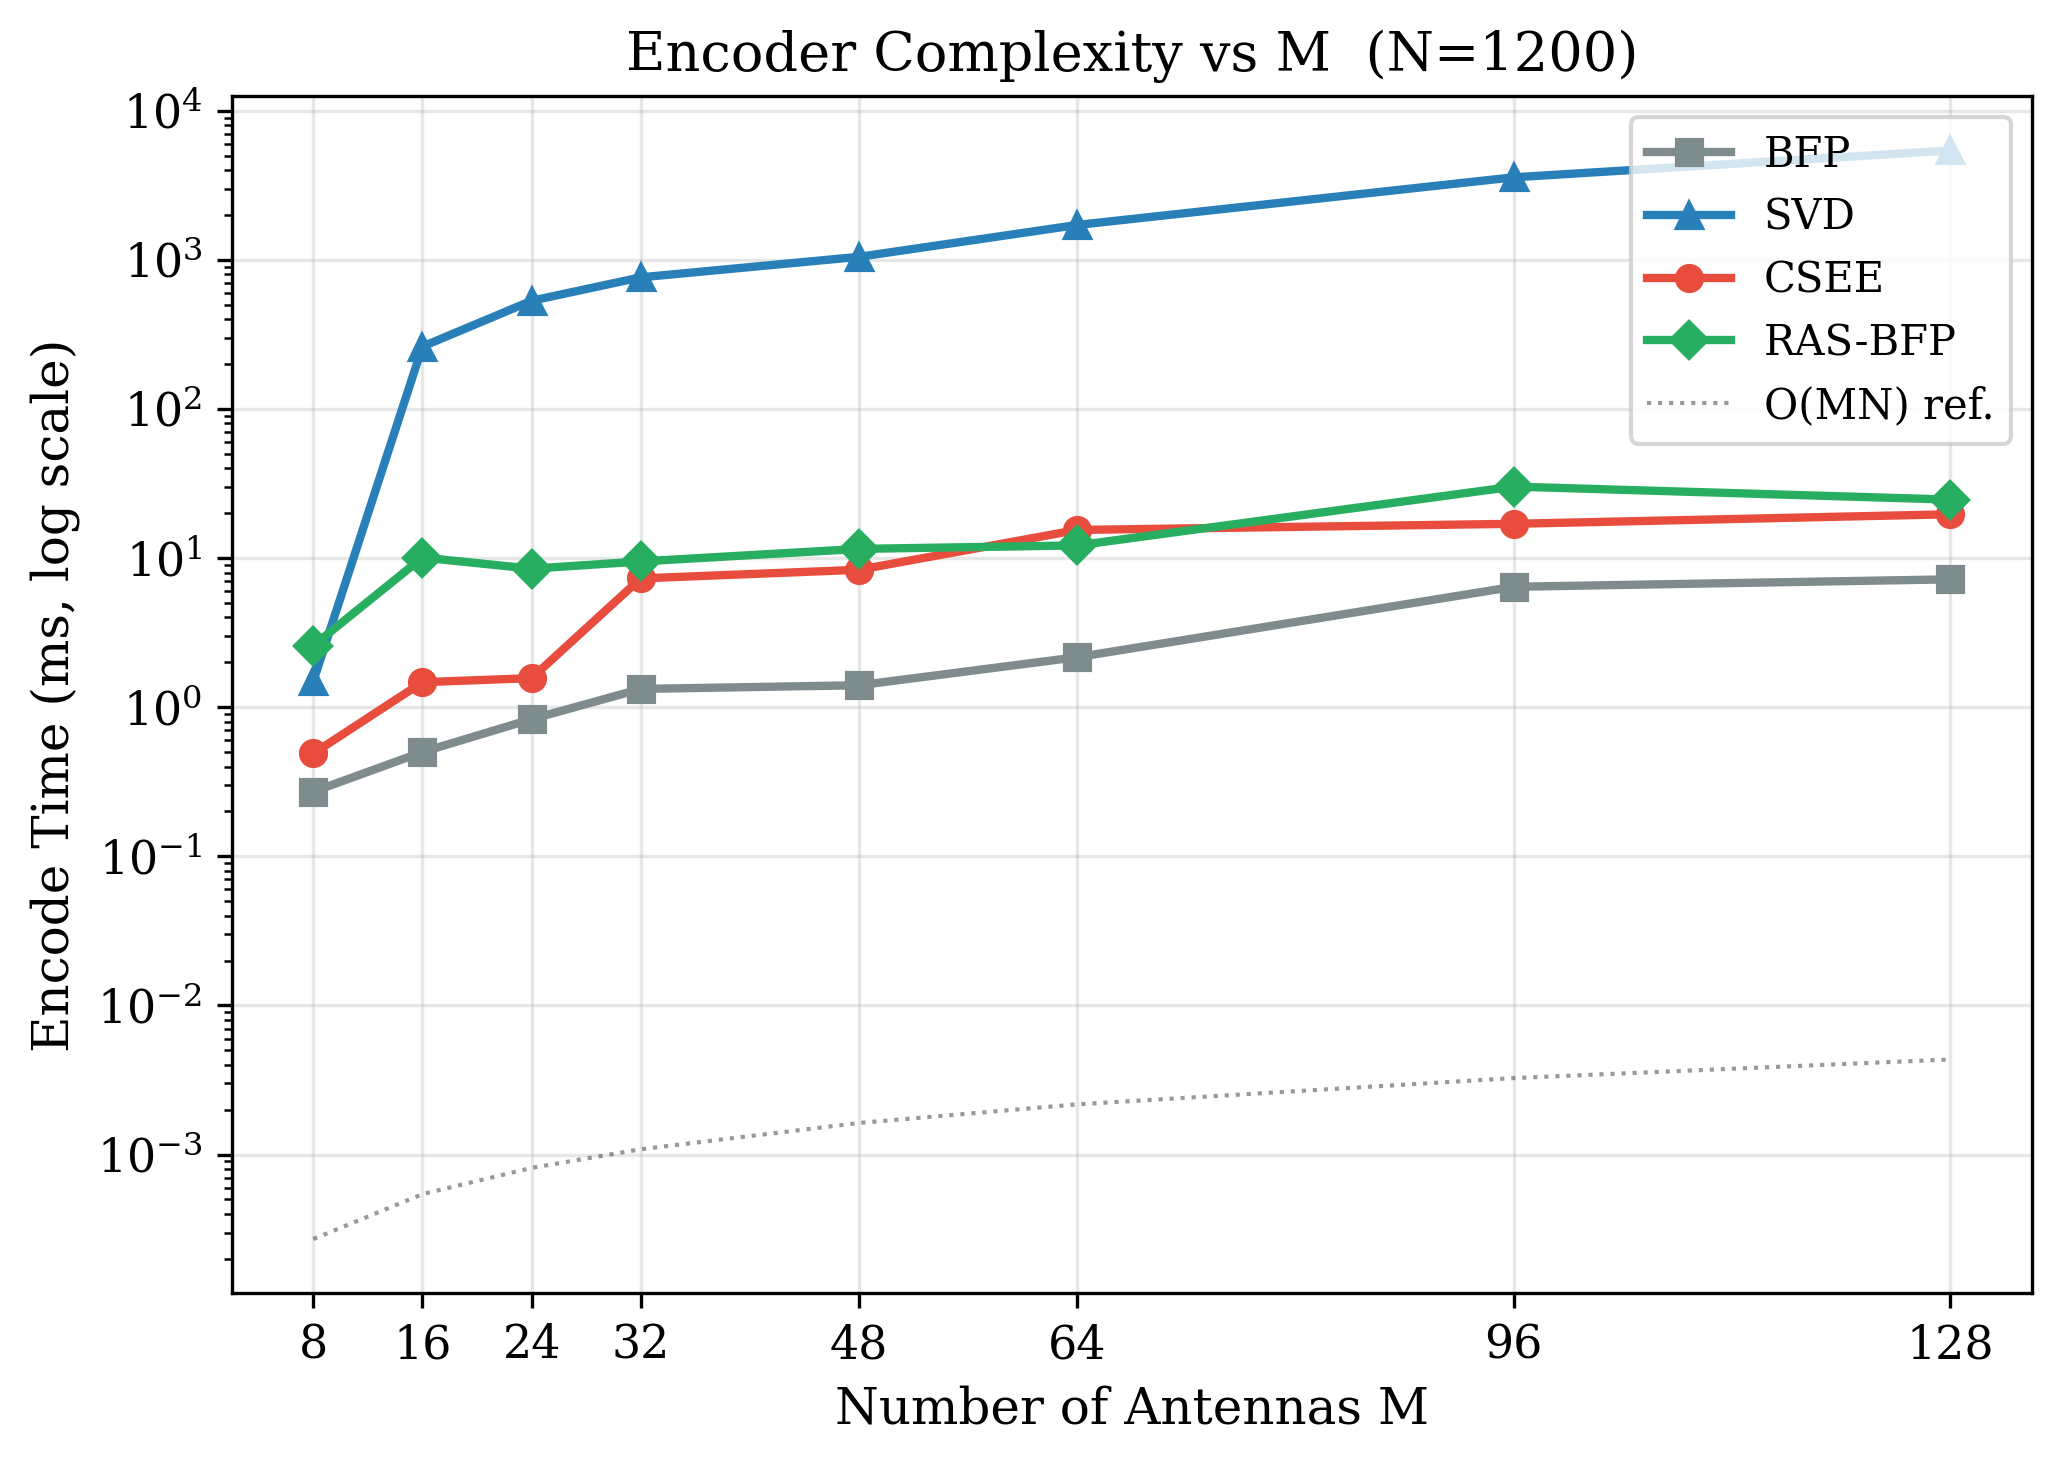
\includegraphics[width=\linewidth]{exp2_complexity.png}
\caption{Encode time versus array size.}
\label{fig:exp2}
\end{subfigure}\hfill
\begin{subfigure}{0.49\textwidth}
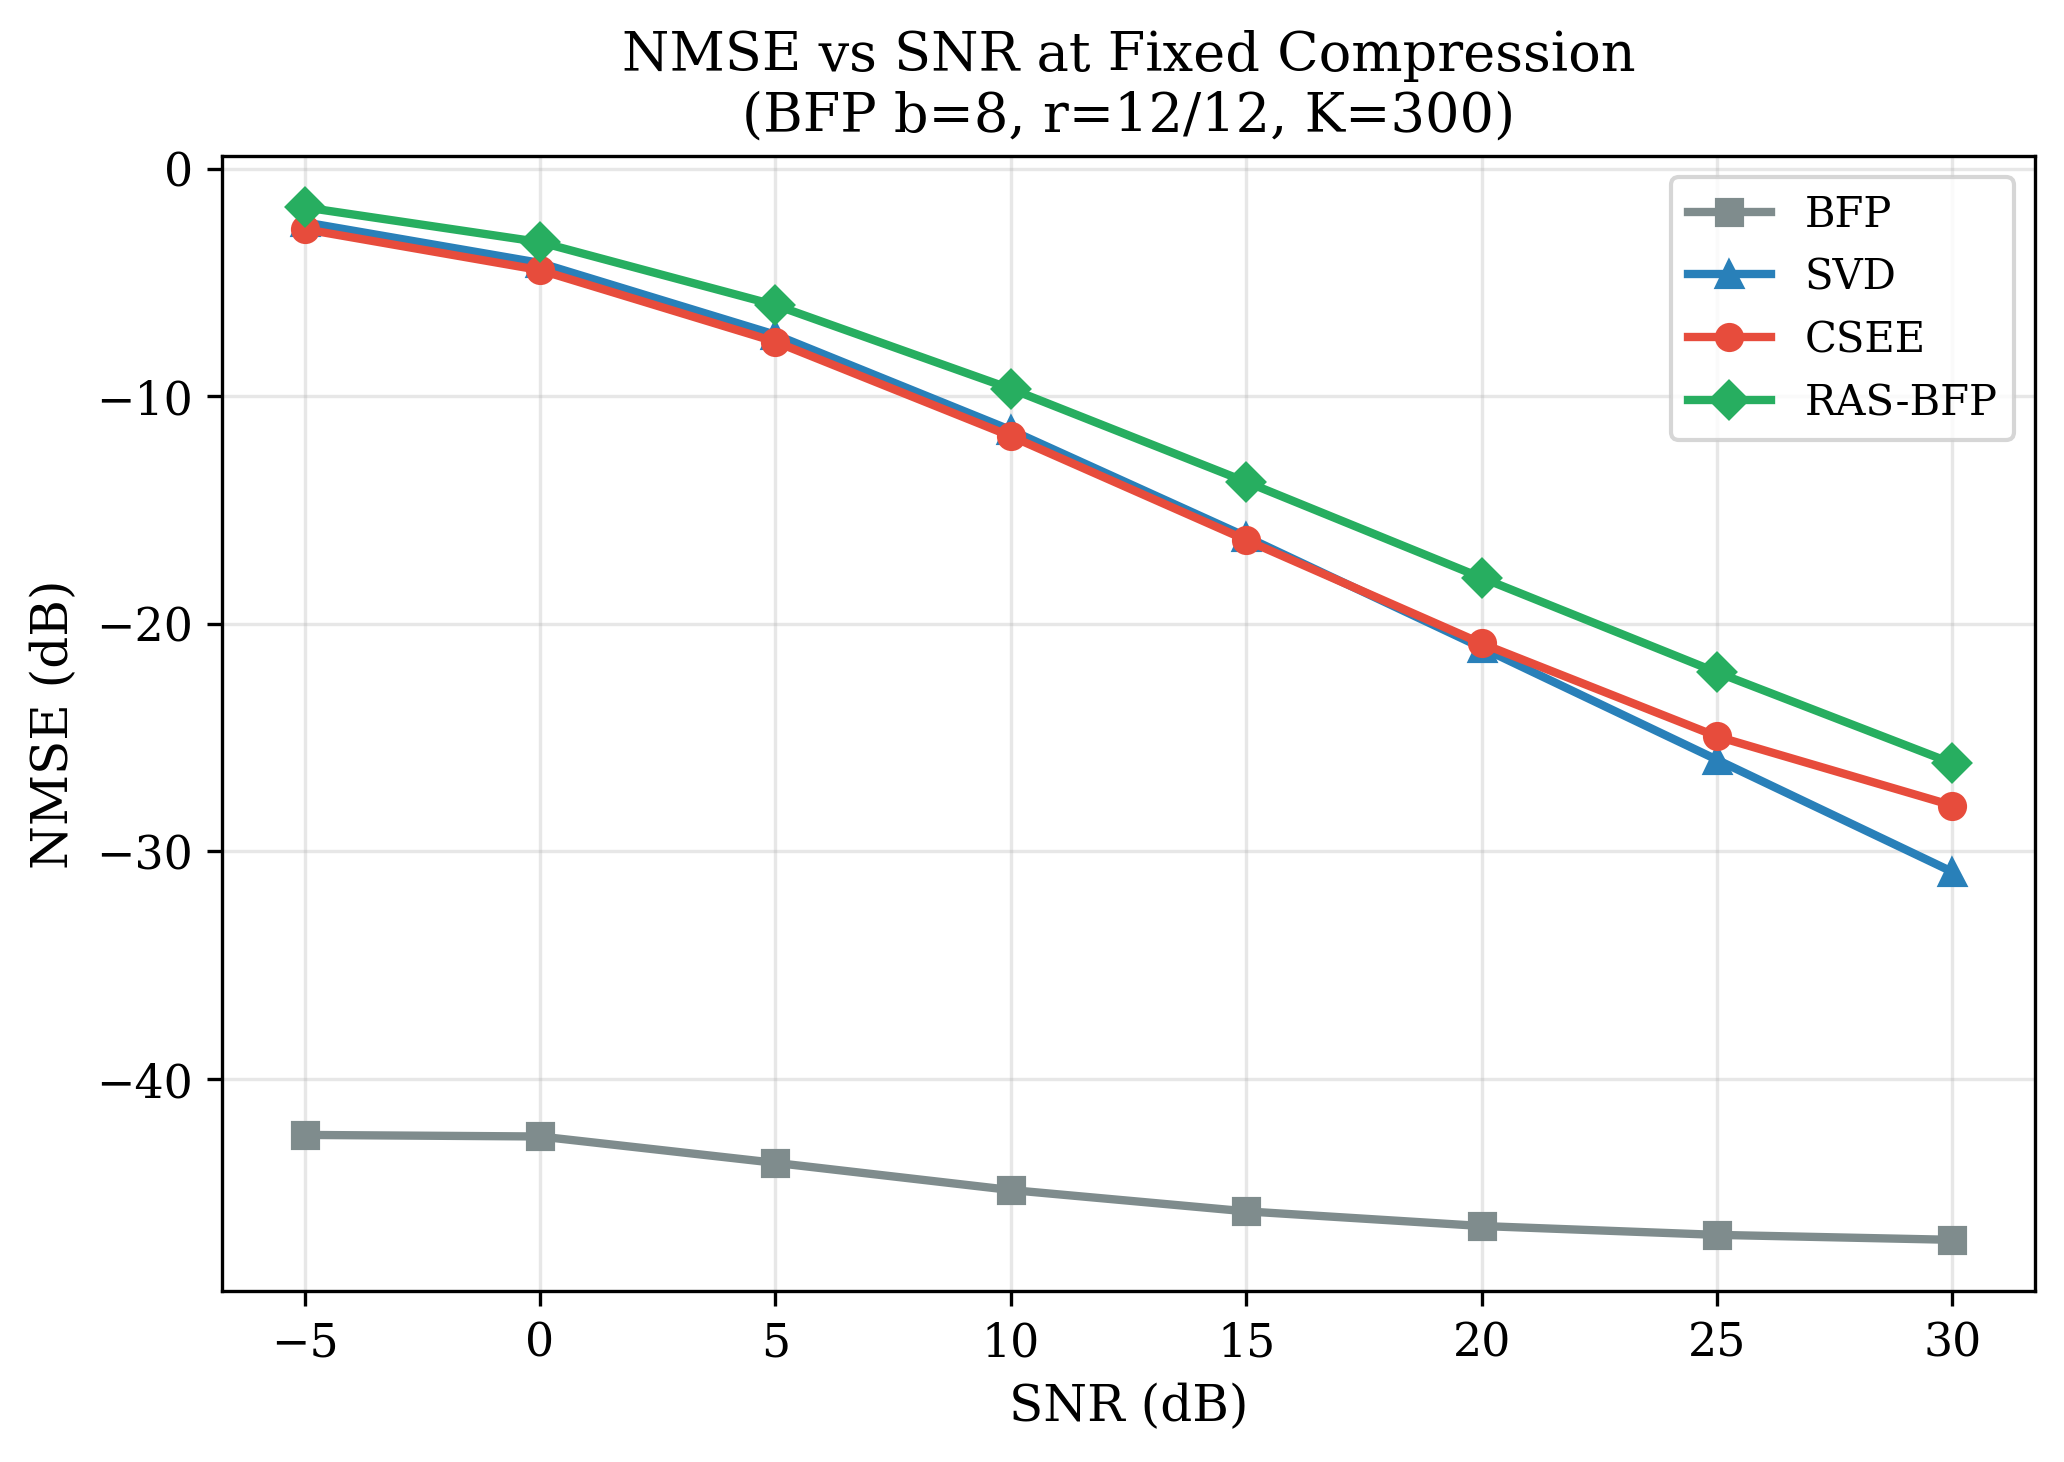
\includegraphics[width=\linewidth]{exp4_snr_sweep.png}
\caption{NMSE versus SNR.}
\label{fig:exp4}
\end{subfigure}
\caption{Complexity and SNR robustness of the encoders: the proposed methods scale near-linearly and keep their accuracy across SNR.}
\end{figure}

\section{Matrix-Inversion Benchmark Results}
\label{sec:ra-bench}

Table~\ref{tab:a-bench} lists the mean and 95th-percentile latency on the held-out matrices of size $n = 100$. Every method is timed through the same Python call path, one matrix per call, so per-call overhead is part of every number and the table ranks methods as they would be used from a Python control loop. In this setting InverseNet-Ultra has the lowest mean latency of the eight methods (0.47~ms) and a 2$\times$ lower 95th percentile than LAPACK (0.57 vs 1.13~ms). It is 2.7$\times$ faster than classical Newton--Schulz and 7$\times$ faster than LU (scipy). The main outcome of the screening is the choice of method family: a Newton--Schulz iteration with a good initial guess, which RMT-WS develops for the complex precoding workload below and Chapter~\ref{ch:impl} implements in C.

\begin{table}[H]
\caption{Inversion screening benchmark on held-out real matrices $A = G/\sqrt n + 2I$, $n = 100$ (CPU, Python, one matrix per call).}
\label{tab:a-bench}
\centering
\begin{tabular}{lcc}
\toprule
Method & Mean & p95 \\
\midrule
\ours \textbf{InverseNet-Ultra (ours)} & \textbf{0.47~ms} & \textbf{0.57~ms} \\
LAPACK \texttt{getri} (numpy) & 0.57~ms & 1.13~ms \\
\ours InverseNet-NS (ours) & 0.97~ms & 1.06~ms \\
Newton--Schulz & 1.27~ms & 1.71~ms \\
Gauss--Jordan & 1.97~ms & 3.40~ms \\
LU (scipy) & 3.36~ms & 6.09~ms \\
SVD & 10.2~ms & 20.8~ms \\
QR & 20.3~ms & 64.5~ms \\
\bottomrule
\end{tabular}
\end{table}

The learned iteration works because it keeps the Newton--Schulz structure and learns only its coefficients: it needs a handful of parameters, generalises across matrices, and a fixed number of batched matrix multiplications gives a flat, predictable latency. This principle, \emph{keep the mathematical structure and learn only what is uncertain}, leads directly to RMT-WS and, in Part~B, to the KKT newsvendor rule.

\section{RMT-WS Results on Complex Precoding Channels}
\label{sec:ra-rmtws}

\subsection{Spectral interval}

Figure~\ref{fig:mp}(a) confirms that the spectrum of the equilibrated Gram matrix follows the Marchenko--Pastur law for i.i.d.\ channels. Table~\ref{tab:a-interval} and Figure~\ref{fig:mp}(b) compare how often the interval $[a,b]$ contains the true spectrum. Our moment-matched interval covers the upper edge in 100\,\% of cases on every channel type and gives 2$\times$ better lower-edge coverage than the classical fixed-ratio bound on strongly correlated and line-of-sight channels, with only $K^2$ work.

\begin{table}[H]
\caption{Probability that $[a,b]$ contains the true spectrum (24 subcarriers $\times$ 30 drops).}
\label{tab:a-interval}
\centering\small
\begin{tabular}{lcc|cc}
\toprule
& \multicolumn{2}{c|}{Fixed-ratio MP + Weyl} & \multicolumn{2}{c}{\textbf{Moment-matched MP (ours)}} \\
Channel & lower edge & upper edge & lower edge & upper edge \\
\midrule
i.i.d., equal gain & 98.9\,\% & 99.3\,\% & \textbf{100\,\%} & \textbf{100\,\%} \\
UMa near-far & 99.6\,\% & 99.9\,\% & \textbf{100\,\%} & \textbf{100\,\%} \\
12$^\circ$ angular spread + near-far & 96.8\,\% & 99.4\,\% & \textbf{100\,\%} & \textbf{100\,\%} \\
3$^\circ$ angular spread + near-far & 61.1\,\% & 94.7\,\% & \textbf{90.6\,\%} & \textbf{100\,\%} \\
Rician 6~dB + 12$^\circ$ & 41.3\,\% & 90.7\,\% & \textbf{84.0\,\%} & \textbf{100\,\%} \\
\bottomrule
\end{tabular}
\end{table}

\begin{figure}[H]
\centering
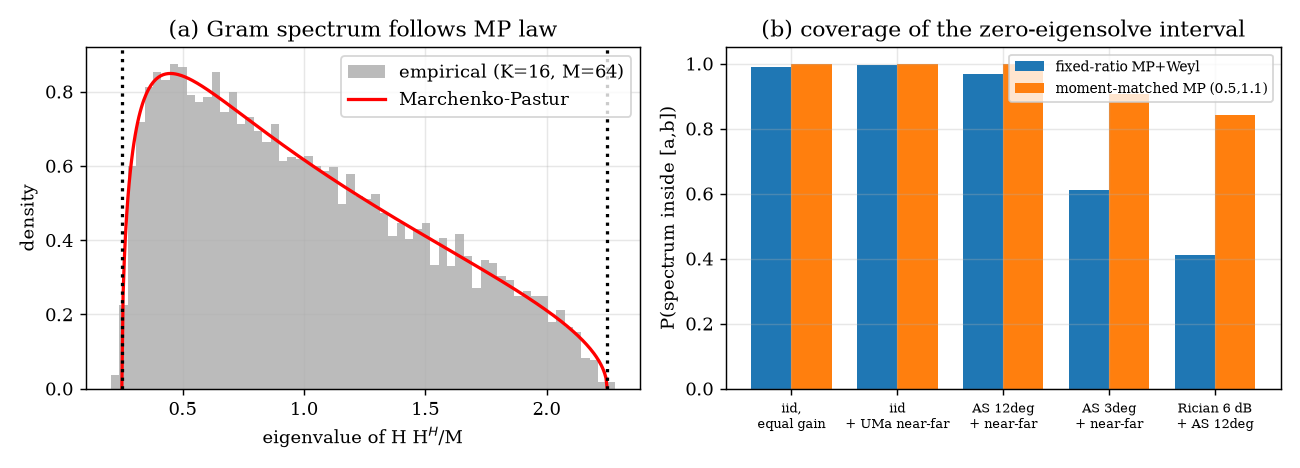
\includegraphics[width=\textwidth]{exp5_spectrum_probability.png}
\caption{(a) The Gram spectrum follows the Marchenko--Pastur law; (b) coverage of the eigensolve-free interval: the moment-matched interval (orange) adapts to correlation and line-of-sight where the fixed-ratio bound (blue) fails.}
\label{fig:mp}
\end{figure}

\subsection{Cold-start inversion cost}

Table~\ref{tab:a-cold} counts the complex GEMMs ($K^3$ multiply-accumulates each) needed to reach at most 1\,\% RZF sum-rate loss. The Chebyshev--MP initialisation followed by Newton--Schulz converges in 6 GEMMs where Neumann-type and classical Newton schemes need more than 10, beats every Neumann/Newton-type scheme, and is the best of all methods at heavy load ($K/M = 0.5$: 9 versus 12 GEMMs).

\begin{table}[H]
\caption{Complex GEMMs needed for $\le 1\,\%$ sum-rate loss (cold start), configurations $M/K$.}
\label{tab:a-cold}
\centering
\begin{tabular}{lcc}
\toprule
Method & 64/16 & 64/32 \\
\midrule
Neumann series (Wu / Prabhu~\cite{wu2013,prabhu2013}) & $>8$ & $>8$ \\
Joint Newton--Neumann (Shao~\cite{shao2016}) & $>10$ & $>10$ \\
Newton--Schulz, classical initialisation & $>10$ & $>10$ \\
Block conjugate gradient & 7 & 12 \\
Gauss--Seidel & 6 & $>12$ \\
\ours \textbf{Chebyshev-MP + Newton--Schulz (ours)} & \textbf{6} & \textbf{9} \\
\bottomrule
\end{tabular}
\end{table}


\subsection{Warm-start tracking across user speeds}

Table~\ref{tab:a-track} and Figure~\ref{fig:exp7} compare RMT-WS with warm-started Gauss--Seidel and conjugate gradient at 3, 30 and 120~km/h ($K=16$, $M=64$). At pedestrian speed RMT-WS needs 2.7$\times$ fewer GEMMs than a cold start at 30$\times$ lower loss; at 30~km/h it has the lowest loss of all warm-started methods; at 120~km/h it has 24$\times$ lower loss than warm Gauss--Seidel. Fixed one- or two-step warm starts diverge at 120~km/h, whereas the certificate makes RMT-WS fall back to a cold start and never diverge: one method serves every speed. It is cheap when users are slow and safe when they are fast.

\begin{table}[H]
\caption{Tracking: sum-rate loss versus exact RZF / GEMMs per slot per PRB ($K=16$, $M=64$).}
\label{tab:a-track}
\centering
\begin{tabular}{lccc}
\toprule
Speed & Warm Gauss--Seidel $\times 4$ & Warm CG $\times 4$ & \textbf{RMT-WS (ours)} \\
\midrule
3~km/h & 0.009\,\% / 4 & 0.013\,\% / 5 & \textbf{0.006\,\% / 2.25} \\
30~km/h & 0.63\,\% / 4 & 0.96\,\% / 5 & \textbf{0.43\,\% / 5.2} \\
120~km/h & 2.9\,\% / 4 & 5.5\,\% / 5 & \textbf{0.12\,\% / 6.25} \\
\bottomrule
\end{tabular}
\end{table}

\begin{figure}[H]
\centering
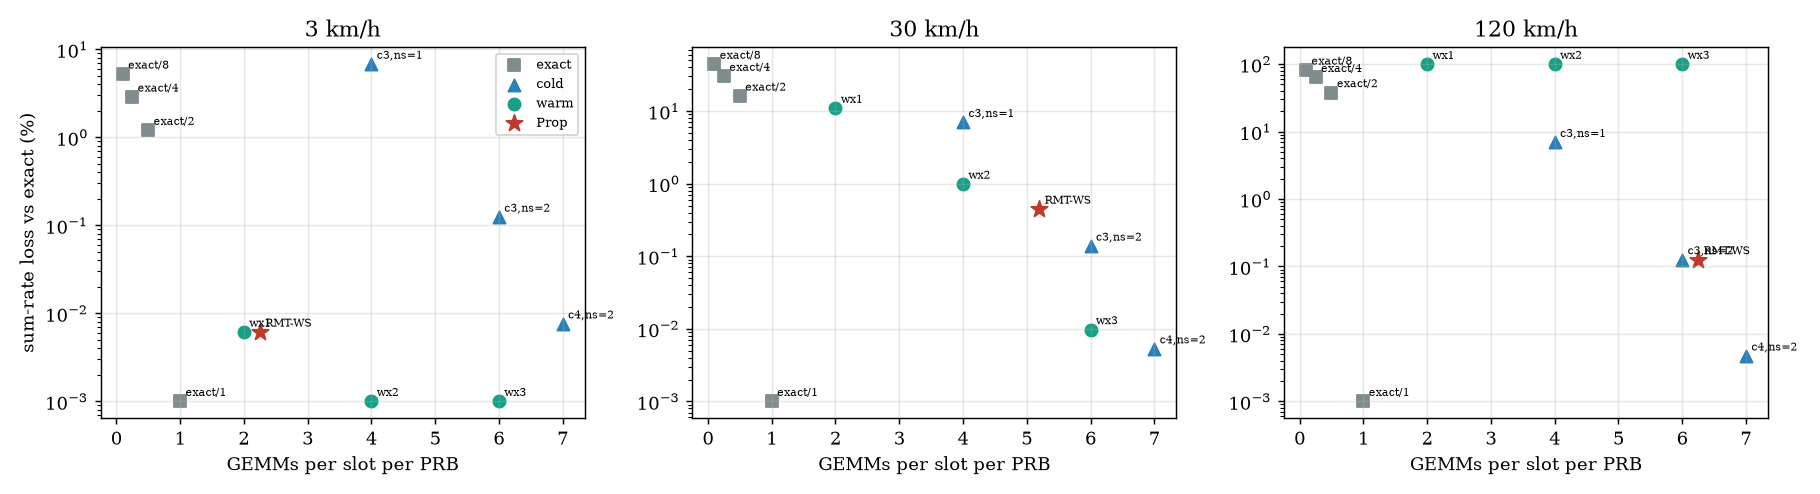
\includegraphics[width=\textwidth]{exp7_tracking.png}
\caption{Tracking accuracy versus cost at 3, 30 and 120~km/h; RMT-WS (red star) sits at the low-cost, low-loss corner at every speed.}
\label{fig:exp7}
\end{figure}

\subsection{Doppler law and certificate}

Figure~\ref{fig:exp12} validates the Doppler-to-warm-start law of Eq.~\eqref{eq:doppler}: the measured initial residual grows linearly with user speed (log-log slope 1.00), and the predicted number of Newton steps matches the measurement. The law gives the DU an explicit warm-start envelope (39~km/h for $M=64$, $K=16$). In an audit of 480 PRB cases from 3 to 120~km/h, zero warm starts accepted by the certificate at $\hat r \le 0.3$ were non-contractive.

\begin{figure}[H]
\centering
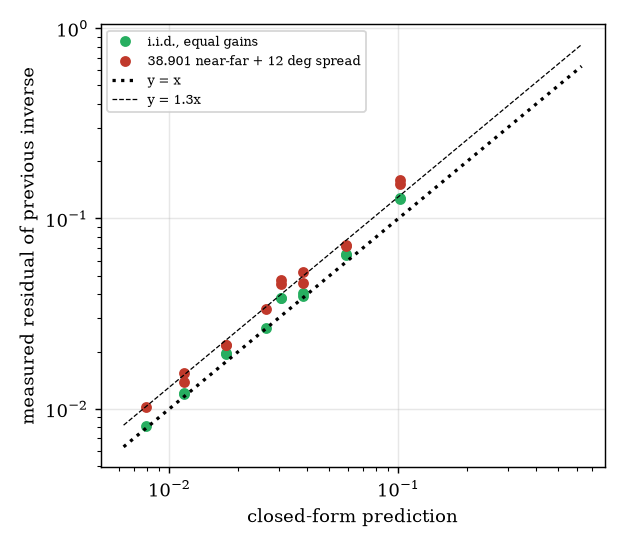
\includegraphics[width=0.62\textwidth]{exp12_doppler_law.png}
\caption{Doppler-to-warm-start law: the initial residual grows linearly with user speed, as predicted.}
\label{fig:exp12}
\end{figure}

\subsection{Robustness at low precision}

Accelerators such as tensor cores and NPUs compute GEMMs with low-precision operands and wide accumulation. Table~\ref{tab:a-lowprec} and Figure~\ref{fig:exp8} show that our Chebyshev + 3 Newton--Schulz inversion keeps 6$\times$ lower loss than direct Gauss--Jordan inversion at 8 mantissa bits and 3.6$\times$ lower at 6 bits, because each Newton step corrects the rounding error of the previous one. The tracker at 8 bits loses only 0.70\,\% against 0.54\,\% at full precision at 30~km/h. RMT-WS is therefore ready for low-precision accelerators where direct inversion degrades.

\begin{table}[H]
\caption{Sum-rate loss versus float64 exact inversion at low precision.}
\label{tab:a-lowprec}
\centering
\begin{tabular}{lcc}
\toprule
Setting & Direct Gauss--Jordan & \textbf{Ours (Chebyshev + 3 NS)} \\
\midrule
8 mantissa bits & 0.88\,\% & \textbf{0.15\,\%} \\
6 mantissa bits & 5.1\,\% & \textbf{1.4\,\%} \\
Ill-conditioned, 10 bits & 1.2\,\% & \textbf{0.49\,\%} \\
\bottomrule
\end{tabular}
\end{table}

\begin{figure}[H]
\centering
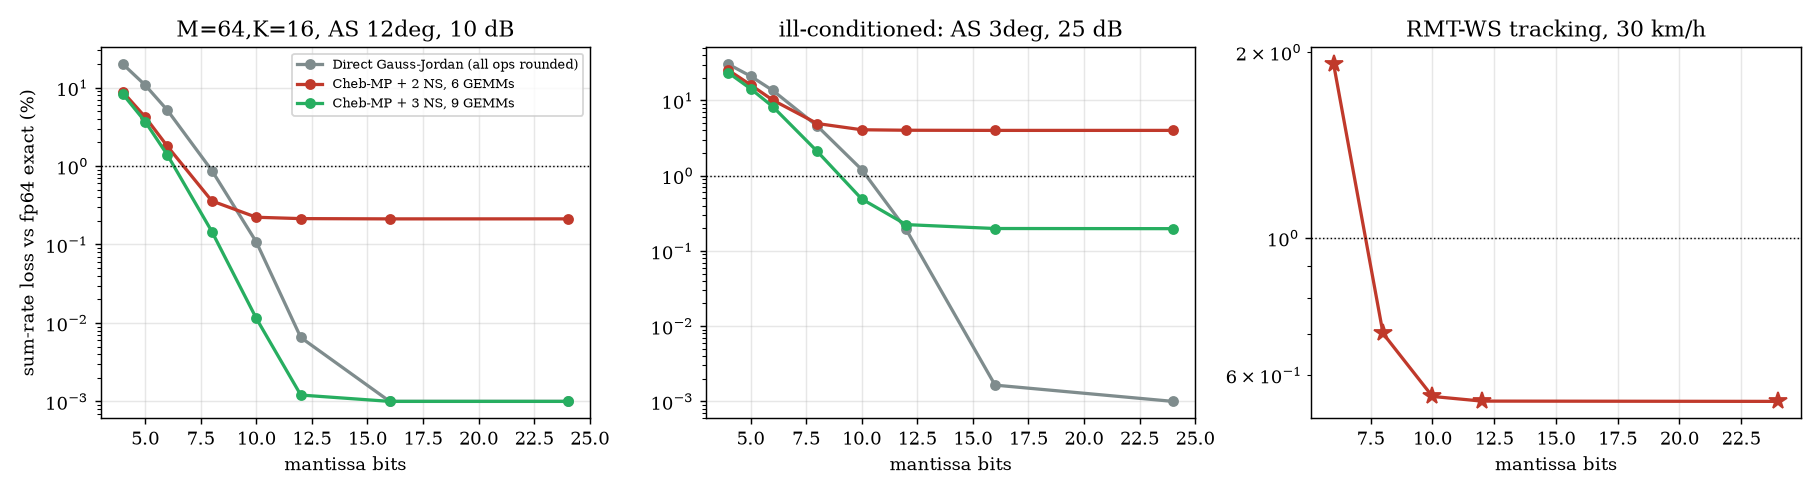
\includegraphics[width=0.85\textwidth]{exp8_low_precision.png}
\caption{Sum-rate loss versus mantissa bits: Newton refinement keeps the loss low where direct inversion degrades.}
\label{fig:exp8}
\end{figure}

\subsection{Comparison with existing complex-inversion methods}

Table~\ref{tab:a-vs-sota} collects the head-to-head comparisons. On every compared metric RMT-WS and its fused kernel are better than the listed existing method.

\begin{table}[H]
\caption{RMT-WS against existing complex-inversion methods.}
\label{tab:a-vs-sota}
\centering\small
\renewcommand{\arraystretch}{1.12}
\begin{tabularx}{\textwidth}{>{\raggedright\arraybackslash}X>{\raggedright\arraybackslash}p{3.6cm}cc}
\toprule
Existing method & Metric & Existing & \textbf{RMT-WS (ours)} \\
\midrule
Neumann series~\cite{wu2013,prabhu2013} & GEMMs for $\le 1\,\%$ loss & $>8$ & \textbf{6} \\
Joint Newton--Neumann~\cite{shao2016} & GEMMs for $\le 1\,\%$ loss & $>10$ & \textbf{6} \\
Newton--Schulz, classical init.~\cite{benisrael1966,pan1991} & GEMMs for $\le 1\,\%$ loss & $>10$ & \textbf{6} \\
Gauss--Seidel & GEMMs, $K/M = 0.5$ & $>12$ & \textbf{9} \\
Block conjugate gradient & GEMMs, $K/M = 0.5$ & 12 & \textbf{9} \\
Warm-started Gauss--Seidel $\times 4$ & loss at 120~km/h & 2.9\,\% & \textbf{0.12\,\%} \\
Warm-started CG $\times 4$ & loss at 30 / 120~km/h & 0.96 / 5.5\,\% & \textbf{0.43 / 0.12\,\%} \\
Fixed 1-/2-step warm start & loss at 120~km/h & diverges & \textbf{0.13\,\%} \\
Direct Gauss--Jordan, 8-bit & sum-rate loss & 0.88\,\% & \textbf{0.15\,\%} \\
Classical MP + Weyl interval & lower-edge coverage, Rician & 41\,\% & \textbf{84\,\%} \\
numpy + LAPACK (whole precoder) & time per slot, $K=16$ & 3.21~ms & \textbf{0.226~ms} \\
\bottomrule
\end{tabularx}
\end{table}

\section{Fronthaul Impact of RU-Side Precoding}
\label{sec:ra-ru}

Table~\ref{tab:a-ru} and Figure~\ref{fig:exp10} quantify the architectures of Figure~\ref{fig:ru-prec} for a 100~MHz carrier with $M=64$, $K=16$ and BFP-9 IQ. Precoding at the radio unit with 8-bit weights refreshed every slot cuts the fronthaul from 118.4 to 32.8~Gbit/s ($-72\,\%$, 3.6$\times$ lighter) at 99.7\,\% of the exact RZF sum-rate. Refreshing the weights less often is not an option at mobility (every 4 slots gives only 70\,\% of the rate at 30~km/h), so per-slot weights are required, and this is exactly the workload our fast precoder handles.

\begin{table}[H]
\caption{Fronthaul rate and sum-rate by precoding architecture (100~MHz, $M=64$, $K=16$, BFP-9).}
\label{tab:a-ru}
\centering
\begin{tabular}{lcc}
\toprule
Architecture & Fronthaul & Sum-rate vs exact \\
\midrule
DU precodes, sends 64 streams & 118.4~Gbit/s & 100\,\% \\
\ours \textbf{RU precodes, 16 layers + 8-bit weights} & \textbf{32.8~Gbit/s ($-72\,\%$)} & \textbf{99.7\,\%} \\
RU precodes, 16 layers + 6-bit weights & 32.0~Gbit/s ($-73\,\%$) & 96.7\,\% \\
\bottomrule
\end{tabular}
\end{table}

\begin{figure}[H]
\centering
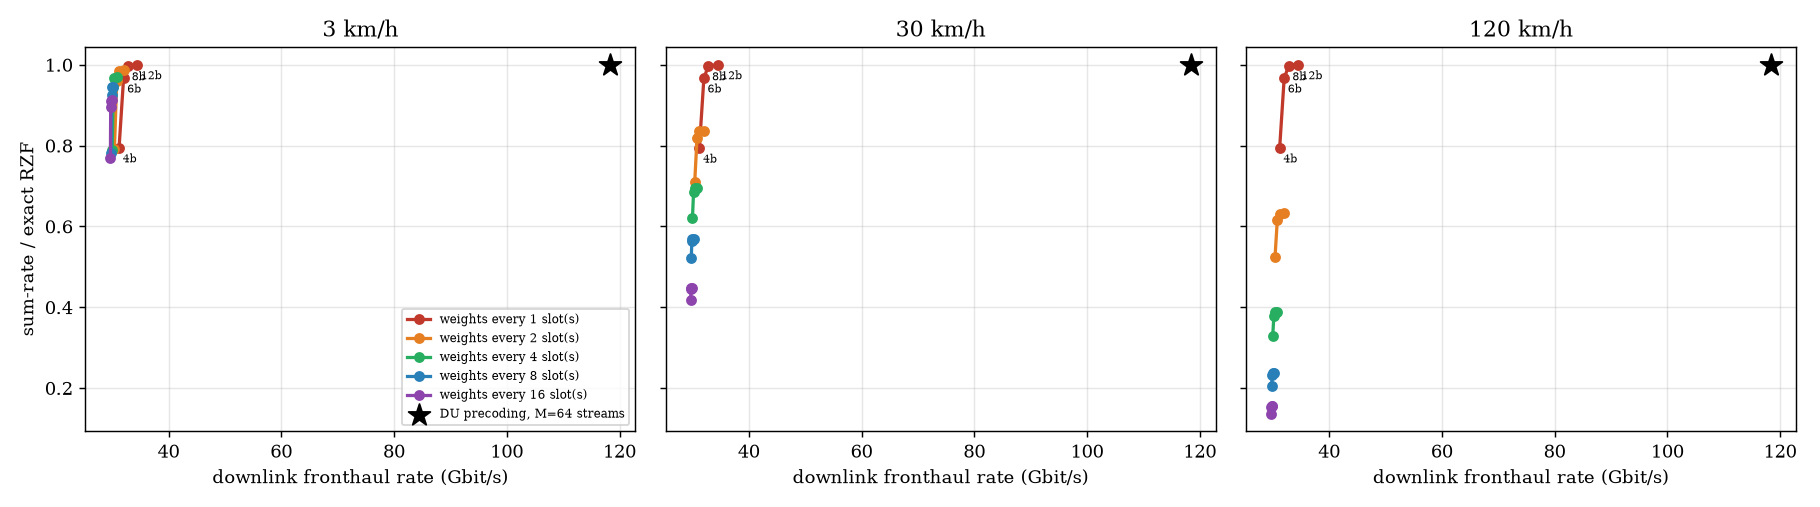
\includegraphics[width=0.9\textwidth]{exp10_fronthaul.png}
\caption{Fronthaul rate and sum-rate by precoding architecture and weight refresh period.}
\label{fig:exp10}
\end{figure}

\section{Summary}

This chapter presented the simulation results of Part~A. The structure-aware encoders compress reference-symbol and channel IQ 6.4--8.1$\times$ against 16-bit I/Q (32$\times$ at the CSEE knee), 3--4 times the ratio of the O-RAN standard, and run 3--6$\times$ faster than SVD. The inversion screening selected a learned Newton--Schulz family, with the lowest mean and a 2$\times$ lower tail latency than LAPACK at $n = 100$. RMT-WS inverts realistic complex Grams in 6 GEMMs instead of more than 10, tracks users at every speed with a certificate that never accepted an unsafe step, and is robust at 8-bit precision. Together with the fused kernel of Chapter~\ref{ch:impl} it enables RU-side precoding with a 72\,\% lighter fronthaul at 99.7\,\% of the exact sum-rate.

% =====================================================================
\chapter{Part B: System Model and Proposed Methods}
\label{ch:partb-methods}
\thispagestyle{plain}
% =====================================================================

\section{Introduction}

Part~A reduces the number of bits each cell puts on the fronthaul. Part~B deals with what happens when even the compressed load is larger than a shared link, and decides how that link is divided among the cells. We built this work in stages, and each stage was a response to a weakness found in the one before it (Figure~\ref{fig:b-roadmap}):
\begin{itemize}
  \item \textbf{B1: the KKT newsvendor rule.} We forecast each cell's \emph{deadline-feasible rate} as a range and split the link so that every cell carries the same priority-weighted risk. This rule is our NCC 2027 submission. Among the 12 reference controllers of that comparison it was the best on two traffic families. That set did not yet include the strongest baselines of the next step, and those baselines do beat it.
  \item \textbf{Extended study.} Here we wrote the problem as a POMDP, developed a Markov-fluid theory of the deadline-feasible rate and added a third traffic family. We also implemented the two strongest baselines we could find in queueing control and policy search, namely predictive MaxWeight and a policy learned by the cross-entropy method.
  \item \textbf{B2: a Bayesian, link-aware Transformer forecaster (LCQT).} This forecaster is designed for the shared link. It has a Bayesian mixture layer and a differentiable KKT layer.
  \item \textbf{B3: the back-pressure newsvendor (BPN).} This is a two-stage policy that contains both strongest baselines exactly. It orders cells by back-pressure and then adds newsvendor margins, and it beats both baselines in all 10 scenarios of three traffic families.
\end{itemize}

\begin{figure}[H]
\centering
\begin{tikzpicture}[font=\footnotesize,>=Stealth,
   s/.style={draw,rounded corners,align=center,text width=3.15cm,minimum height=2.2cm,inner sep=4pt}]
  \node[s,fill=iitblue!10] (b1) {\textbf{B1}\\KKT newsvendor rule\\[2pt]\scriptsize $\rstar$ target, GBM quantiles, closed-form split};
  \node[s,fill=orange!12,right=0.45cm of b1] (ext) {\textbf{Extended study}\\theory + baselines\\[2pt]\scriptsize POMDP, Markov-fluid bounds, Family M, pred.\ MaxWeight, CEM};
  \node[s,fill=purple!10,right=0.45cm of ext] (b2) {\textbf{B2}\\Bayesian LCQT\\[2pt]\scriptsize patch + cross-cell Transformer, mixture, diff.\ KKT};
  \node[s,fill=good!15,right=0.45cm of b2,draw=good!60!black,thick] (b3) {\textbf{B3}\\Back-pressure newsvendor\\[2pt]\scriptsize contains both strongest baselines; wins 10/10};
  \draw[->,thick] (b1) -- (ext);
  \draw[->,thick] (ext) -- (b2);
  \draw[->,thick] (b2) -- (b3);
\end{tikzpicture}
\caption{Development of the Part~B controllers. Each step keeps the structure that works and adds what the previous step was missing.}
\label{fig:b-roadmap}
\end{figure}

\section{Problem Setting and System Model}
\label{sec:b-model}

\subsection{Cells, link and decision}

Eight 7-2x cells share one 25~Gbit Ethernet aggregation link (Figure~\ref{fig:shared}). Three of them are low-latency (LL) cells with a deadline of 2~ms and priority weight 3. The other five are eMBB cells with a deadline of 10~ms and weight 1. We reserve 3\,\% of the link for the control, management and synchronisation planes, which leaves a capacity of $C = 12.125$~Mbit per 0.5~ms slot. The peak demands of the cells add up to $2.44\,C$. This over-subscription is deliberate. Operators do the same in practice to gain from statistical multiplexing.

A coordinator acts every $T = 20$ slots (10~ms). At each decision it sets a budget $r_i$ (bits per slot) for every cell, and that budget stays fixed for the whole interval. The coordinator sees the cells' queues, head-of-line ages, demand history and spectral efficiency, but only after a telemetry delay of $\tau = 2$ slots (1~ms). Each budget must therefore cover a lead time of $H = T + \tau$ slots that the coordinator has not observed (Figure~\ref{fig:timing}).

\begin{figure}[H]
\centering
\begin{tikzpicture}[font=\footnotesize,>=Stealth]
  \draw[->,thick] (0,0) -- (13,0) node[right]{slots};
  \foreach \x in {0,0.5,...,12.5} \draw (\x,-0.07) -- (\x,0.07);
  \draw[fill=orange!25] (2.0,0.25) rectangle (3.0,0.75); \node at (2.5,0.5) {$\tau$};
  \draw[fill=iitblue!15] (3.0,0.25) rectangle (13.0,0.75); \node at (8.0,0.5) {budgets $r_i$ held for $T = 20$ slots (10\,ms)};
  \draw[->,thick,accent] (2.0,1.4) -- (2.0,0.8); \node[text=accent,align=center] at (2.0,1.75) {telemetry\\snapshot};
  \draw[->,thick,good!60!black] (3.0,1.4) -- (3.0,0.8); \node[text=good!50!black,align=center] at (3.6,1.75) {decision\\epoch $t_k$};
  \draw[decorate,decoration={brace,amplitude=5pt,mirror}] (2.0,-0.3) -- (13.0,-0.3) node[midway,below=6pt]{lead time $H = T + \tau$: arrivals unseen when deciding};
\end{tikzpicture}
\caption{Timing of one control interval. The budgets are fixed on 1~ms-old telemetry and must cover the next $H = T+\tau$ slots of unseen traffic.}
\label{fig:timing}
\end{figure}

We did not choose to decide in advance. Real deployments force it. Near-real-time RIC and E2 control loops run at 10~ms or slower, and traffic shaping in a switch is not reconfigured every slot. The DU schedulers of different cells also have no way to consult each other inside the sub-millisecond processing pipeline.

\subsection{Fronthaul demand}

With $b$-bit BFP, one PRB-layer costs the following number of fronthaul bits per slot:
\begin{equation}
  \beta(b) = (12\cdot 2\cdot b + 8)\cdot 14\cdot\kappa,
  \label{eq:beta}
\end{equation}
where $\kappa = 1.08$ is the packet overhead. This gives $\beta(9) = 3387$ bits, and 6-, 12- and 14-bit mantissas scale this by $0.68$, $1.32$ and $1.54$. \emph{Part~A enters Part~B at this point}, because the compression setting fixes $\beta$ and with it the load. A cell with user bits $a_i(t)$ and spectral efficiency $\eta_i(t)$ (bits per PRB-layer) then has fronthaul demand
\begin{equation}
  d_i(t) = \lceil a_i(t)/\eta_i(t)\rceil\,\beta,
\end{equation}
so the fronthaul load of two cells with the same user traffic can differ by a factor of 2--3. A full cell (273 PRBs, 4 layers) peaks at about 7.4~Gbit/s.

\subsection{Constraints, queues and metric}

The budgets satisfy
\begin{equation}
  \sum_i r_i \le C, \qquad 0 \le r_i \le \mathrm{cap}_i = 273\,L_i\,\beta .
\end{equation}
Each cell keeps a FIFO queue at the DU. Bits that wait longer than $D_i$ slots are dropped and counted as \emph{deadline violations}. The budgets already respect the capacity, so the link itself never builds a queue. Congestion shows up instead as queueing and drops at the DU. Our primary metric was fixed before any tuning. It is the priority-weighted violation ratio
\begin{equation}
  V_w = \frac{\sum_i w_i\,\mathrm{violated}_i}{\sum_i w_i\,\mathrm{arrived}_i},
\end{equation}
in which a dropped LL bit counts three times. Alongside it we report per-class violations, link utilisation, unused allocation, DU delay, Jain fairness and decision time.

\section{Key Idea 1: the Deadline-Feasible Rate}
\label{sec:rstar}

What should a forecaster predict? The traffic volume is the obvious choice, but it is the wrong one, since a 2~ms cell hit by a burst needs far more than its average rate. We instead forecast the smallest constant rate at which no bit misses its deadline.

\begin{definition}[Deadline-feasible rate]
For arrivals $a_1,\dots,a_H$ and deadline $D$ slots,
\begin{equation}
  \rstar(a, D) = \max_{1\le s\le e\le H} \frac{\sum_{t=s}^{e} a_t}{e - s + 1 + D}.
  \label{eq:rstar}
\end{equation}
\end{definition}

Eq.~\eqref{eq:rstar} is the service-curve condition of network calculus~\cite{leboudec2001}. It says that every window of arrivals must be served within its own length plus the deadline. The condition is tight, and our tests confirm this to within one PRB-layer. When the deadline is long, bursts can be smoothed out and $\rstar$ approaches the mean rate. When it is short, $\rstar$ approaches the peak burst rate. Take a single burst of 8 units with an average of 1 per slot. It needs $\rstar = 8/2 = 4$ for $D=1$ slot, but only $8/8 = 1$ for $D=7$ slots (Figure~\ref{fig:rstar}). In our 2~ms cells $\rstar$ is usually 2--3$\times$ the mean, and its distribution is strongly right-skewed.

\begin{figure}[H]
\centering
\begin{tikzpicture}[font=\footnotesize,>=Stealth,xscale=0.75,yscale=0.42]
  \draw[->] (0,0) -- (13.5,0) node[right]{slot};
  \draw[->] (0,0) -- (0,9.2) node[above]{bits};
  \foreach \x/\h in {1/0,2/0,3/8,4/0,5/0,6/0,7/0,8/0} \draw[fill=iitblue!40] (\x-0.4,0) rectangle (\x+0.4,\h);
  \node[iitblue] at (3,8.6) {burst $=8$};
  \draw[very thick,accent] (3-0.5,4) -- (4.5,4) node[right,font=\scriptsize]{$D=1$: $\rstar = 8/2 = 4$};
  \draw[very thick,good!60!black] (3-0.5,1) -- (10.5,1) node[right,font=\scriptsize]{$D=7$: $\rstar = 8/8 = 1$};
\end{tikzpicture}
\caption{The deadline-feasible rate of one burst for a short and a long deadline: a short deadline forces a rate close to the peak.}
\label{fig:rstar}
\end{figure}

All deadline-aware controllers request the same quantity,
\begin{equation}
  \text{need}_i = B_i + \rstar_i, \qquad B_i = \frac{\text{backlog}_i}{\text{slack}_i},
\end{equation}
which is the rate needed to clear the current queue before its deadline, plus $\rstar_i$ for traffic that has not arrived yet. The controllers differ only in how they estimate $\rstar_i$ and in how they split a shortage. A single number is a poor basis for reserving a skewed quantity, so we forecast a \emph{range}.

\section{Key Idea 2: a Quantile Forecaster}
\label{sec:gbm}

The target is $y_i = \rstar(d_i[t-\tau : t+T], D_i)/\mathrm{cap}_i$, which is the deadline-feasible rate of the coming horizon divided by the cell's peak. All 28 features are computed from past slots. They are the last six horizon means (with their mean, standard deviation and maximum), two exponentially weighted averages, the last four slot demands, $\rstar$ of the last three horizons, the relative spectral efficiency, $D_i/H$ and a one-hot cell identifier. Normalisation uses configuration constants only. For each level $\alpha \in \{0.05, 0.25, 0.5, 0.75, 0.9, 0.95\}$ we train one histogram gradient-boosting quantile regressor (300 trees, 15 leaves) on 101k rows from 16 training traces. Training takes 12~s on a CPU. The training, validation and test seeds do not overlap (1000--1015, 2000--2003 and 3000--3019).

\section{Key Idea 3: the KKT (Constrained Newsvendor) Rule}
\label{sec:kkt}

\subsection{Objective and solution}

Suppose each cell comes with a forecast distribution $F_i$ of $\rstar_i$. We then maximise the expected priority-weighted need served in the interval,
\begin{equation}
  \max_{r}\ \sum_i w_i\,\mathbb{E}\big[\min(B_i + \rstar_i,\ r_i)\big]
  \quad \text{s.t.}\ \sum_i r_i \le C,\ \ 0\le r_i\le \mathrm{cap}_i .
  \label{eq:nv}
\end{equation}
The function $\mathbb{E}[\min(B_i + \rstar_i, r)]$ is concave in $r$. Its derivative is $w_i\,(1 - F_i(r - B_i))$, the weighted probability that the last bit of budget is actually used. Because the problem is separable and concave, the KKT conditions give its \emph{global} optimum in closed form:
\begin{equation}
  \boxed{\; r_i(\lambda) = \mathrm{clip}\Big(B_i + F_i^{-1}\big(1 - \lambda/w_i\big),\ 0,\ \mathrm{cap}_i\Big)\;}
  \label{eq:kkt}
\end{equation}
Only one scalar has to be found. It is $\lambda \ge 0$, the shadow price of link capacity, and a 60-step bisection chooses it so that $\sum_i r_i(\lambda) = C$. If the link is not full, $\lambda = 0$ and every cell gets its full predictive support. We interpolate $F_i^{-1}$ piecewise-linearly through the six forecast quantiles. The cost is $O(NK + N n_{\rm iter})$, which comes to a few tens of microseconds for eight cells.

\paragraph{Interpretation.} Eq.~\eqref{eq:kkt} cuts every cell at the \emph{same priority-weighted risk}. A cell with a wide forecast or a high priority gets a larger margin above its backlog, while a cell with a confident forecast gets roughly its median. Nobody tunes these margins by hand. They are \emph{derived} from the forecast and the link constraint.

\paragraph{Toy example.} Say the bisection returns $\lambda = 0.6$. An LL cell ($w=3$) is then funded up to the $1 - 0.6/3 = 0.8$ quantile of its forecast, and an eMBB cell ($w=1$) up to its $1-0.6 = 0.4$ quantile (Figure~\ref{fig:kkt-toy}).

\begin{figure}[H]
\centering
\begin{tikzpicture}[font=\footnotesize,>=Stealth,yscale=0.9]
  \draw[->] (0,0) -- (9.6,0);
  \draw[->] (0,0) -- (0,4.6) node[above]{budget $r_i$};
  % cells
  \foreach \x/\b/\m/\lab/\col in {1/0.8/2.4/LL 1/accent,2.6/0.5/2.0/LL 2/accent,4.2/1.3/0.6/eMBB 1/iitblue,5.8/0.4/0.9/eMBB 2/iitblue,7.4/0.9/0.4/eMBB 3/iitblue}{
    \draw[fill=gray!35] (\x-0.45,0) rectangle (\x+0.45,\b);
    \draw[fill=\col!30] (\x-0.45,\b) rectangle (\x+0.45,\b+\m);
    \node[below] at (\x,0) {\lab};
  }
  \node[align=left,anchor=west,font=\scriptsize] at (8.1,3.9) {\tikz\draw[fill=gray!35] (0,0) rectangle (0.3,0.2); backlog $B_i$};
  \node[align=left,anchor=west,font=\scriptsize] at (8.1,3.4) {\tikz\draw[fill=accent!30] (0,0) rectangle (0.3,0.2); LL: $F^{-1}(0.8)$};
  \node[align=left,anchor=west,font=\scriptsize] at (8.1,2.9) {\tikz\draw[fill=iitblue!30] (0,0) rectangle (0.3,0.2); eMBB: $F^{-1}(0.4)$};
  \node[align=left,anchor=west,font=\scriptsize] at (8.1,2.2) {$\textstyle\sum_i r_i = C$\\one price $\lambda = 0.6$};
\end{tikzpicture}
\caption{Illustration of the KKT rule: every cell first receives its backlog rate, then a quantile of its forecast whose level is set by its priority and a common capacity price $\lambda$.}
\label{fig:kkt-toy}
\end{figure}

\subsection{Properties}

We prove four properties of the rule. The proofs are in Appendix~\ref{app:proofs}.

\begin{proposition}[Feasibility]\label{prop:feas}
For any forecast and any $\lambda$, the budgets satisfy the caps, and the bisection output satisfies $\sum_i r_i \le C$: the link is never overloaded.
\end{proposition}

\begin{proposition}[Equal weighted tail probability]\label{prop:equal}
At an interior optimum, $w_i\big(1 - F_i(r_i - B_i)\big) = \lambda$ for every cell. With point forecasts (degenerate $F_i$), the rule reduces to a priority-ordered fill.
\end{proposition}

\begin{proposition}[Backlog first]\label{prop:backlog}
Any cell with $\lambda < w_i$ receives at least $\min(B_i,\mathrm{cap}_i)$ before the uncertain demand of any cell of equal or lower weight is funded.
\end{proposition}

\begin{proposition}[Robustness to miscalibration]\label{prop:robust}
If $\sup_x |F_i(x) - G_i(x)| \le \epsilon$ for every cell, where $G_i$ is the true distribution, then
\begin{equation}
  J_G(r^G) - J_G(r^F) \le \epsilon\sum_i w_i\big[(r_i^G - B_i)^+ + (r_i^F - B_i)^+\big] \le 2\,\epsilon\, w_{\max}\, C .
\end{equation}
The loss due to a miscalibrated forecast grows at most linearly in $\epsilon$.
\end{proposition}

\subsection{Control loop}

Figure~\ref{fig:loop} shows the full loop, which runs every 10~ms. We handle the edge cases explicitly. If a forecast is not finite, the controller falls back to window quantiles. A cell with zero demand gets zero budget plus a share of any headroom. When the link is not binding, every cell gets its full predictive support.

\begin{figure}[H]
\centering
\begin{tikzpicture}[font=\footnotesize,>=Stealth,node distance=0.5cm and 0.45cm,
   st/.style={draw,rounded corners,fill=iitblue!10,align=center,minimum height=1.1cm,text width=2.55cm}]
  \node[st] (obs) {Delayed state ($t-\tau$):\\queues, HOL age,\\history, $\eta$};
  \node[st,right=of obs] (feat) {28 features\\per cell};
  \node[st,right=of feat] (gbm) {Forecaster:\\quantiles of $\rstar_i$};
  \node[st,right=of gbm,fill=accent!12] (kkt) {Allocation rule\\(KKT / BPN)};
  \node[st,below=1.1cm of kkt,fill=good!12] (du) {DU schedulers:\\$\lfloor r_i/\beta\rfloor$ PRB-layers\\per slot};
  \node[st,left=of du] (link) {Shared link\\(never overloaded)};
  \node[st,left=of link] (q) {FIFO queues,\\drops after $D_i$};
  \node[st,left=of q] (traffic) {Traffic\\$a_i(t)$, $\eta_i(t)$};
  \draw[->,thick] (obs) -- (feat);
  \draw[->,thick] (feat) -- (gbm);
  \draw[->,thick] (gbm) -- (kkt);
  \draw[->,thick] (kkt) -- node[right,font=\scriptsize]{$r_i$ held $T$ slots} (du);
  \draw[->,thick] (du) -- (link);
  \draw[->,thick] (link) -- (q);
  \draw[->,thick] (traffic) -- (q);
  \draw[->,thick,dashed] (q.north) to[out=110,in=-70] (obs.south);
  \node[above=0.08cm of kkt,text=iitblue] {every $T = 10$\,ms};
\end{tikzpicture}
\caption{The closed control loop of Part~B. The forecaster and the allocation rule are the two blocks developed in this chapter.}
\label{fig:loop}
\end{figure}

\section{Extended Study: Theory and the Strongest Baselines}
\label{sec:ext}

\subsection{The control problem as a POMDP}

Let the state be $s(t) = (Q(t), Z(t), \eta(t))$, which collects the queue age profiles, the hidden traffic state and the spectral efficiencies. At epochs $t_k = kT$ the controller solves
\begin{equation}
  \min_{\pi}\ \mathbb{E}_\pi\Big[\sum_k \sum_{t=t_k}^{t_k+T-1} \sum_i w_i\,\mathrm{dropped}_i(t)\Big],
  \qquad r(t_k) = \pi\big(s(t_k - \tau),\text{history}\big).
\end{equation}
This partially observable MDP cannot be solved directly. Its continuous state has hundreds of dimensions, the traffic law is unknown, and each action is held for $T$ slots. We implemented the three main families of approximations instead:
\begin{enumerate}
  \item \textbf{One-step stochastic programs.} The KKT newsvendor rule (Section~\ref{sec:kkt}) applied to a learned or model-based distribution, including a Markov chain fitted online.
  \item \textbf{Lyapunov drift.} MaxWeight~\cite{tassiulas1992} and \textbf{predictive MaxWeight}~\cite{huang2016}. The latter serves cells in order of $w_i\,(Q_i + \ell H m_i)$, the queue the cell \emph{will} have given forecast median $m_i$, and gives each cell up to $Q_i/T + (1+\mu)\,m_i$.
  \item \textbf{Direct policy search.} A class-level policy in which each cell reserves $B_i + F_i^{-1}(p_{c(i)})$ and any shortage is shared by weighted water-filling with a learned LL weight. Its three parameters $(p_{\rm LL}, p_{\rm eMBB}, w_{\rm LL})$ are learned on training seeds with the cross-entropy method (CEM)~\cite{rubinstein1999}. One can think of it as a small and reliable analogue of a deep-RL xApp.
\end{enumerate}

\subsection{Markov-fluid theory of the deadline-feasible rate}

Consider Markov-modulated traffic with phase chain $P$ (stationary distribution $\pi$), per-phase log-MGF $\psi_k(\theta)$ and $\Phi(\theta) = \mathrm{diag}(e^{\psi_k(\theta)})$. For this model we derived the following results.
\begin{itemize}
  \item the window log-MGF $\Lambda_l(\theta) = \log\big(\pi^{\mathsf T}\Phi(P\Phi)^{l-1}\mathbf 1\big)$ and the effective bandwidth $\alpha(\theta) = \log\rho(P\Phi(\theta))/\theta$~\cite{kesidis1993,kelly1996};
  \item a \textbf{Chernoff--union bound} on the deadline-feasible rate,
  \begin{equation}
    \Pr(\rstar > x) \le \sum_{l=1}^{H}(H-l+1)\,\min_\theta \exp\big(-\theta x(l+D) + \Lambda_l(\theta)\big);
  \end{equation}
  \item a \textbf{large-deadline decay} $\limsup_{D\to\infty} D^{-1}\log\Pr(\rstar > x) \le -x\,\theta^\ast(x)$, which links $\rstar$ to classical buffer-overflow asymptotics~\cite{anick1982,duffield1994};
  \item a pathwise \textbf{shortfall sandwich} valid for any arrivals,
  \begin{equation}
    (D+1)(\rstar - r)^+ \le V(r) \le \textstyle\sum_t (a_t - r)^+,
  \end{equation}
  where $V(r)$ is the volume violated at constant rate $r$. It follows that the newsvendor surrogate~\eqref{eq:nv} is a lower bound on the violated volume.
\end{itemize}
The bounds held in every validation run. They are, however, conservative by a factor of 25--100 at 2--10~ms deadlines. That gap is a strong reason to \emph{learn} the distribution of $\rstar$ from data instead of computing it from a model.

\section{B2: LCQT, a Bayesian Link-Aware Quantile Transformer}
\label{sec:lcqt}

\subsection{Architecture}

LCQT (Figure~\ref{fig:lcqt}) can replace the GBM forecaster directly. It is assembled from established components: PatchTST patches~\cite{nie2023}, iTransformer-style attention across variates~\cite{liu2024}, TFT-style multi-quantile output~\cite{lim2021}, FiLM conditioning~\cite{perez2018film}, deep ensembles~\cite{lakshminarayanan2017} and MC dropout~\cite{gal2016}. We made six changes to adapt it to the shared fronthaul link.
\begin{enumerate}
  \item \textbf{Deadline-aware patch tokens.} The 352 slots of history are cut into 16 patches of $H=22$ slots. Each patch token carries its own $\rstar$ at the cell's deadline, along with its mean and maximum. A separate summary token holds the 28 GBM features.
  \item \textbf{Deadline/priority FiLM.} A single network serves both LL and eMBB cells and is modulated by $(D_i/H, p_i)$.
  \item \textbf{Link-aware cross-cell attention.} After the temporal encoder, attention runs over the eight cells that share the link.
  \item \textbf{Non-crossing quantile head.} Writing $q_k = q_{k-1} + \mathrm{softplus}(a_k)$ makes the quantiles monotone by construction.
  \item \textbf{Bayesian mixture layer.} Three trained seeds $\times$ eight dropout passes form a posterior, and its \emph{mixture} distribution is what the allocation rule receives.
  \item \textbf{Differentiable KKT layer.} This lets the network be trained through the coupled capacity constraint.
\end{enumerate}
The model has 63k parameters (44k without the cross-cell layer). It uses the same seeds and target as the GBM and trains in about 6 minutes on a 4-core CPU, with 40 epochs of AdamW on a one-cycle schedule and early stopping on validation pinball loss.

\begin{figure}[H]
\centering
\begin{tikzpicture}[font=\scriptsize,>=Stealth,
    box/.style={draw=iitblue,fill=soft,rounded corners=2pt,align=center,minimum height=1.0cm,text width=1.75cm,inner sep=2pt},
    hot/.style={box,draw=accent,fill=accent!8},
    grn/.style={box,draw=good,fill=good!8}]
  \node[box] (hist) {Per-cell history\\$a_i(t)$, 352 slots};
  \node[box,right=0.3cm of hist] (patch) {16 patches\\+ $\rstar$, mean, max};
  \node[box,below=0.35cm of patch] (feat) {Summary token\\28 features};
  \node[box,right=0.3cm of patch] (enc) {Temporal encoder\\2 layers, $d{=}48$\\4 heads};
  \node[box,right=0.3cm of enc] (film) {FiLM\\$(D_i/H,\ p_i)$};
  \node[hot,right=0.3cm of film] (cross) {Cross-cell\\attention\\(8 cells)};
  \node[box,right=0.3cm of cross] (head) {Non-crossing\\6 quantiles};
  \node[grn,below=1.6cm of cross,text width=2.3cm] (bayes) {Bayesian layer\\3 seeds $\times$ 8 dropout\\$\Rightarrow$ mixture $\hat F_i$};
  \node[grn,left=0.6cm of bayes,text width=2.9cm] (kkt) {KKT layer\\$r_i = B_i + \hat F_i^{-1}(1-\lambda^\ast/w_i)$};
  \node[hot,left=0.6cm of kkt,text width=3.2cm] (loss) {Decision loss\\$\sum_i p_i (D_i{+}1)(B_i{+}\rstar_i - r_i)^+$\\$+\ \beta\,$pinball};
  \draw[->] (hist) -- (patch);
  \draw[->] (patch) -- (enc);
  \draw[->] (feat.east) -| ([xshift=-0.2cm]enc.south);
  \draw[->] (enc) -- (film);
  \draw[->] (film) -- (cross);
  \draw[->] (cross) -- (head);
  \draw[->] (head.south) |- (bayes.east);
  \draw[->] (bayes) -- (kkt);
  \draw[->,dashed,accent] (kkt) -- node[above]{$\partial\lambda^\ast$} (loss);
\end{tikzpicture}
\caption{LCQT: link-aware cross-cell quantile Transformer with the Bayesian mixture layer and the differentiable KKT layer used for decision-focused training.}
\label{fig:lcqt}
\end{figure}

\subsection{Bayesian mixture layer}

The posterior samples $s = 1,\dots,MS$ (ensemble members $\times$ dropout passes) each give a quantile function $Q_i^{(s)}$. Averaging their quantiles would throw away the disagreement between samples. We pass the KKT rule the mixture distribution instead,
\begin{equation}
  \hat F_i(x) = \frac{1}{MS}\sum_s F_i^{(s)}(x).
\end{equation}
so a cell whose forecast the posterior is unsure about gets a wider margin at the same price $\lambda^\ast$. Dropout is seeded per decision slot, which keeps runs exactly reproducible.

\subsection{Differentiable KKT layer and decision-focused training}

The forward pass finds $\lambda^\ast$ by bisection. For the backward pass we apply the implicit function theorem to the binding link constraint $g(\lambda,q) = \sum_i r_i(\lambda,q) - C = 0$, which gives
\begin{equation}
  \frac{\partial\lambda^\ast}{\partial q} = -\frac{\partial g/\partial q}{\partial g/\partial \lambda},
\end{equation}
and in code this is one Newton step from the detached root. The decision-focused model (DF-LCQT) is trained on the shortfall-sandwich lower bound of the dropped bits, $\sum_i p_i (D_i+1)(B_i + \rstar_i - r_i)^+$, with a pinball regulariser added. The contexts $(B_i, w_i)$ depend on the policy. For that reason we log them in closed loop on training seeds and refresh them with one DAgger round. Unit tests check that the layer agrees with the numpy allocator to $10^{-6}$. They also check that $\partial \sum_i r_i / \partial q = 0$ when the link is full, since budget can then only move between cells.

\section{B3: The Back-Pressure Newsvendor}
\label{sec:bpn}

\subsection{Motivation}

A budget acts as a per-cell cap. If capacity is reserved for the upper quantile of a 2~ms cell and then goes unused, no other cell can have it. A pure reservation rule protects LL cells well for this reason, but it leaves the eMBB cells short. Back-pressure (MaxWeight) fills the link in order of queue pressure using median demands. It wastes less capacity, yet it ignores both deadlines and forecast uncertainty. The back-pressure newsvendor (BPN) puts the two ideas together. It \emph{fills a base in back-pressure order and then spends the leftover capacity on newsvendor margins} (Figure~\ref{fig:bpn}).

\begin{figure}[H]
\centering
\begin{tikzpicture}[font=\footnotesize,>=Stealth,
   s/.style={draw,rounded corners,align=left,text width=6.2cm,inner sep=5pt}]
  \node[s,fill=iitblue!8] (st1) {\textbf{Stage 1: base in back-pressure order}\\[2pt]
    base rate $b_i = a\,Q_i/T + (1-a)\,B_i$\\
    base demand $d_i = b_i + (1+\mu)\,\hat F_i^{-1}(p^0_{c(i)})$\\
    shortage shared $\propto v_{c}\,(\pi_i/\bar\pi)^{\eta}$\\
    pressure $\pi_i = Q_i + \ell H m_i$\\[2pt]
    \scriptsize $\eta = 0$: class-weighted water-fill (reservation)\\ $\eta = \eta_{\max}$: strict back-pressure order};
  \node[s,fill=good!10,right=0.8cm of st1] (st2) {\textbf{Stage 2: leftover by the KKT rule}\\[2pt]
    $r_i = \max\!\big(r_i^{(1)},\ b_i + \hat F_i^{-1}(1 - \lambda/\omega_{c(i)})\big)$\\
    with $\lambda$ such that $\sum_i r_i = C$\\[2pt]
    \scriptsize newsvendor margins only where the forecast is wide};
  \draw[->,very thick] (st1) -- node[above,font=\scriptsize]{$r^{(1)}$} (st2);
  \node[draw,rounded corners,fill=orange!10,below=0.6cm of st1.south east,anchor=north,xshift=0.4cm,text width=12.8cm,align=center,inner sep=4pt] (cem) {\textbf{Learning:} 8 parameters $\theta = (a, \mu, p^0_{\rm LL}, p^0_{\rm eMBB}, v_{\rm LL}, \eta, \ell, \omega_{\rm LL})$ by CEM on \emph{training} seeds, started from the tuned optimum of each contained baseline};
\end{tikzpicture}
\caption{The two stages of the back-pressure newsvendor and how its parameters are learned.}
\label{fig:bpn}
\end{figure}

\subsection{The policy}

\paragraph{Stage 1.} The base rate $b_i = a\,Q_i/T + (1-a)\,B_i$ blends MaxWeight's queue drain rate with the deadline-aware backlog rate. To get each cell's base demand we add a class-specific base quantile of its forecast, $d_i = b_i + (1+\mu)\hat F_i^{-1}(p^0_{c(i)})$. If the base demands exceed the link, the shortage is shared in proportion to $v_{c}(\pi_i/\bar\pi)^{\eta}$. Here the pressure is $\pi_i = Q_i + \ell H m_i$, the queue plus look-ahead $\times$ forecast median. Changing the exponent $\eta$ moves the policy smoothly from class-weighted water-filling ($\eta = 0$, reservation) to strict back-pressure ordering ($\eta = \eta_{\max}$).

\paragraph{Stage 2.} The KKT rule distributes whatever capacity is left after stage~1. Each cell gets $r_i = \max(r_i^{(1)},\ b_i + \hat F_i^{-1}(1 - \lambda/\omega_{c(i)}))$, and bisection sets $\lambda$ so that $\sum_i r_i = C$.

\subsection{Both strongest baselines are special cases}

For suitable parameters BPN \emph{is} each of the strongest baselines. Unit tests verify this exactly under shortage. The settings are:
\begin{itemize}
  \item predictive MaxWeight: $a = 1$, $p^0 = 0.5$, $\mu$ = its margin, $\eta = \eta_{\max}$;
  \item the CEM class-level policy: $a = 0$, $p^0$ = its class levels, $v_{\rm LL} = w_{\rm LL}$, $\eta = 0$.
\end{itemize}
A search over the BPN parameters that starts from the tuned optimum of each baseline can then only match or improve on both of them.

\subsection{Learning with equal search effort}

We learn the eight parameters with CEM on training seeds only, using 8 episodes per candidate, which is the same search used for the baselines. The search is started twice, once at the tuned optimum of each contained baseline. For a fair comparison, both baselines were also \emph{re-tuned with the same CEM search} (``CEM-tuned''), so every controller had equal tuning effort. Two versions are reported. BPN~v1 has 6 parameters and always uses strict back-pressure in stage~1. BPN~v2 has 8 parameters, adding the sharing exponent $\eta$ and the margin $\mu$, and it contains the reservation policy as well.

\section{Summary}

This chapter developed the Part~B controllers. The deadline-feasible rate turns deadlines into a demand target, and a calibrated quantile forecaster describes how uncertain that target is. The closed-form KKT rule then splits the link at equal priority-weighted risk, and we proved four properties for it. In the extended study we framed the problem as a POMDP, derived Markov-fluid bounds and introduced the strongest baselines. LCQT contributes a link-aware Bayesian Transformer forecaster with a differentiable KKT layer. The back-pressure newsvendor brings reservation and back-pressure into one learned policy class that contains both strongest baselines. Chapter~\ref{ch:partb-results} evaluates all of these methods.

% =====================================================================
\chapter{Part B: Simulation Results}
\label{ch:partb-results}
\thispagestyle{plain}
% =====================================================================

\section{Introduction}

This chapter presents the closed-loop evaluation of the Part~B controllers. Section~\ref{sec:rb-protocol} first describes the traffic families, the reference controllers and the statistical protocol. The B1 results follow in Sections~\ref{sec:rb-main}--\ref{sec:rb-overhead}. They cover the main comparison, the source of the gain, the ablations, the 3GPP traffic family, robustness, the interaction with Part~A compression and the decision overhead. Section~\ref{sec:rb-ext} then reports the extended study and Section~\ref{sec:rb-b2} the Bayesian Transformer forecaster. Section~\ref{sec:rb-b3} covers the back-pressure newsvendor, which is the final and best controller of the project.

\section{Evaluation Protocol}
\label{sec:rb-protocol}

\subsection{Traffic families}

We use three independent traffic families, so that no conclusion rests on a single traffic model:
\begin{itemize}
  \item \textbf{Family S (synthetic, bursty).} Gamma background traffic is combined with ON/OFF bursts whose sojourns are heavy-tailed Pareto ($\alpha_{\rm on} = 1.5$, $\alpha_{\rm off} = 1.8$)~\cite{willinger1997}, together with slow load regimes and drift in spectral efficiency. There are five scenarios: low (offered load 0.50), moderate (0.65), high (0.80), flash crowds, and a \textbf{held-out distribution shift} that is never seen in training or tuning.
  \item \textbf{Family G (standards-based, nothing hand-designed).} The geometry is 3GPP TR 38.901 UMa with 7 interfering sites and Jakes fading~\cite{tr38901}, and channel quality is mapped with the TS 38.214 CQI table~\cite{ts38214}. eMBB cells carry FTP Model~3 traffic~\cite{tr36814}, and LL cells carry XR video at 60~fps~\cite{tr38838}. The fronthaul demand is the output of a round-robin PRB scheduler. We run this family at moderate (0.65) and high (0.80) load.
  \item \textbf{Family M (Markov-modulated).} Gamma sources are modulated by a Markov chain with idle, normal and burst phases. The scenarios are moderate and high load, plus a semi-Markov held-out shift with Pareto sojourns.
\end{itemize}

\subsection{Reference controllers}

\begin{table}[H]
\caption{Controllers of the B1 comparison (all tuned on validation seeds).}
\label{tab:b-controllers}
\centering\small
\setlength{\tabcolsep}{4pt}
\begin{tabular}{lll}
\toprule
Controller & Estimate of $\rstar$ & Allocation \\
\midrule
Static equal & none & $C/N$ \\
Reactive proportional & mean-rate EWMA (deadline-unaware) & proportional water-fill \\
MaxWeight & priority $\times$ queue, HOL-age urgency & max-weight \\
Deadline-aware reactive & last observed $\rstar$ & deadline-weighted water-fill \\
Point forecast & GBM \textbf{median} & deadline-weighted water-fill \\
Fixed global quantile & GBM quantile, one tuned level (0.75) & water-fill \\
Proposed (window) & empirical quantiles, last 30 horizons (no ML) & KKT rule \\
\ours \textbf{Proposed} & \textbf{GBM quantiles} & \textbf{KKT rule} \\
Oracle water-fill & true $\rstar$ (reference only) & water-fill \\
Oracle + KKT & true $\rstar$ (reference only) & KKT rule \\
\bottomrule
\end{tabular}
\end{table}

Table~\ref{tab:b-controllers} lists the controllers of the B1 comparison. The point forecast is the most important ablation, since it uses the same model but passes on only one number. The fixed global quantile is included to check that simply reserving a high quantile is not what makes the method work. For every baseline we tuned the margins $\{0, 0.25, 0.5\}$, the EWMA windows and the persistence windows on validation seeds, and a margin of 0 turned out best for all of them. All baselines redistribute unused capacity and share the weights, backlog rate and water-fill of the point-forecast controller. The oracles use the true future $\rstar$ and serve only as references. The extended study adds predictive MaxWeight, the CEM policy, a model-based Markov-chain KKT rule, a bound-quantile KKT rule and a tuned-weight KKT rule, which brings the total to 19 controllers.

\subsection{Statistical protocol}

Each scenario is run for 20 test seeds of 20{,}000 slots (10~s), after 1{,}000 warm-up slots. All controllers receive the same traces and the same stale observations. The train, validation and test seeds do not overlap, and every forecaster is frozen before testing starts. Most of the variation from seed to seed comes from burst timing, which all controllers share, so we report paired per-seed comparisons. For each pair we give the mean relative change of $V_w$ with a 95\,\% bootstrap confidence interval, the number of seeds won out of 20, and a Wilcoxon signed-rank test with Holm correction. The simulation parameters are collected in Table~\ref{tab:b-params}.

\begin{table}[H]
\caption{Part~B simulation parameters.}
\label{tab:b-params}
\centering\small
\begin{tabular}{ll}
\toprule
Parameter & Value \\
\midrule
Cells & 8: 3 LL ($D = 2$~ms, $w = 3$), 5 eMBB ($D = 10$~ms, $w = 1$) \\
Link & 25GE, 3\,\% reserved $\Rightarrow C = 12.125$~Mbit per 0.5~ms slot \\
Over-subscription & $\sum_i$ peak$_i = 2.44\,C$ \\
Per-cell peak & 273 PRBs $\times$ 4 layers $\times\ \beta(9)$ $\approx$ 7.4~Gbit/s \\
Control interval, delay & $T = 20$ slots (10~ms), $\tau = 2$ slots (1~ms) \\
Forecast quantiles & 0.05, 0.25, 0.5, 0.75, 0.9, 0.95 \\
Seeds & train 1000--1015, validation 2000--2003, test 3000--3019 \\
Test length & 20 seeds $\times$ 20{,}000 slots after 1{,}000 warm-up \\
Statistics & paired bootstrap 95\,\% CI, Holm-corrected Wilcoxon \\
\bottomrule
\end{tabular}
\end{table}

\section{B1: Main Result on Family S}
\label{sec:rb-main}

Table~\ref{tab:b-main} lists $V_w$ for every controller in every scenario. Among the implementable controllers, the proposed KKT rule is best in all five scenarios, and this includes flash crowds and the held-out shift. At high load it reaches 8.00\,\%. The point forecast gives 9.70\,\% at the same load, reactive proportional 9.20\,\% and MaxWeight 11.54\,\%. Figure~\ref{fig:b-main} plots the same data.

\begin{table}[H]
\caption{B1 main result, Family S: $V_w$ [\%] (mean $\pm$ std over 20 test seeds; lower is better).}
\label{tab:b-main}
\centering\scriptsize
\setlength{\tabcolsep}{3.5pt}
\begin{tabular}{lccccc}
\toprule
Method & low 0.50 & moderate 0.65 & high 0.80 & flash crowds & shift (held-out) \\
\midrule
Static equal share & 4.45 $\pm$ 1.05 & 9.65 $\pm$ 1.36 & 15.46 $\pm$ 1.51 & 19.15 $\pm$ 2.34 & 22.31 $\pm$ 2.99 \\
Reactive proportional & 0.83 $\pm$ 0.27 & 4.11 $\pm$ 0.69 & 9.20 $\pm$ 0.99 & 12.27 $\pm$ 2.23 & 11.70 $\pm$ 2.24 \\
MaxWeight & 0.90 $\pm$ 0.28 & 4.85 $\pm$ 0.79 & 11.54 $\pm$ 1.27 & 15.24 $\pm$ 3.02 & 12.31 $\pm$ 2.44 \\
Deadline-aware reactive & 0.52 $\pm$ 0.21 & 4.24 $\pm$ 0.78 & 11.03 $\pm$ 1.33 & 14.51 $\pm$ 3.06 & 12.56 $\pm$ 2.81 \\
Point forecast (GBM median) & 0.27 $\pm$ 0.17 & 3.23 $\pm$ 0.73 & 9.70 $\pm$ 1.34 & 13.33 $\pm$ 3.09 & 11.30 $\pm$ 2.81 \\
Fixed global quantile (0.75) & 0.34 $\pm$ 0.23 & 4.35 $\pm$ 1.02 & 11.76 $\pm$ 1.44 & 15.09 $\pm$ 3.17 & 12.85 $\pm$ 3.32 \\
Proposed, window quantiles (no ML) & 0.25 $\pm$ 0.13 & 2.57 $\pm$ 0.64 & 8.72 $\pm$ 1.34 & 12.67 $\pm$ 3.19 & 10.22 $\pm$ 2.88 \\
\ours \textbf{Proposed (GBM + KKT)} & \textbf{0.15 $\pm$ 0.13} & \textbf{2.15 $\pm$ 0.60} & \textbf{8.00 $\pm$ 1.27} & \textbf{11.76 $\pm$ 3.08} & \textbf{10.04 $\pm$ 2.71} \\
\midrule
\textcolor{gray}{Oracle water-fill (reference)} & \textcolor{gray}{0.07} & \textcolor{gray}{1.62} & \textcolor{gray}{6.89} & \textcolor{gray}{10.16} & \textcolor{gray}{6.69} \\
\bottomrule
\end{tabular}
\end{table}

\begin{figure}[H]
\centering
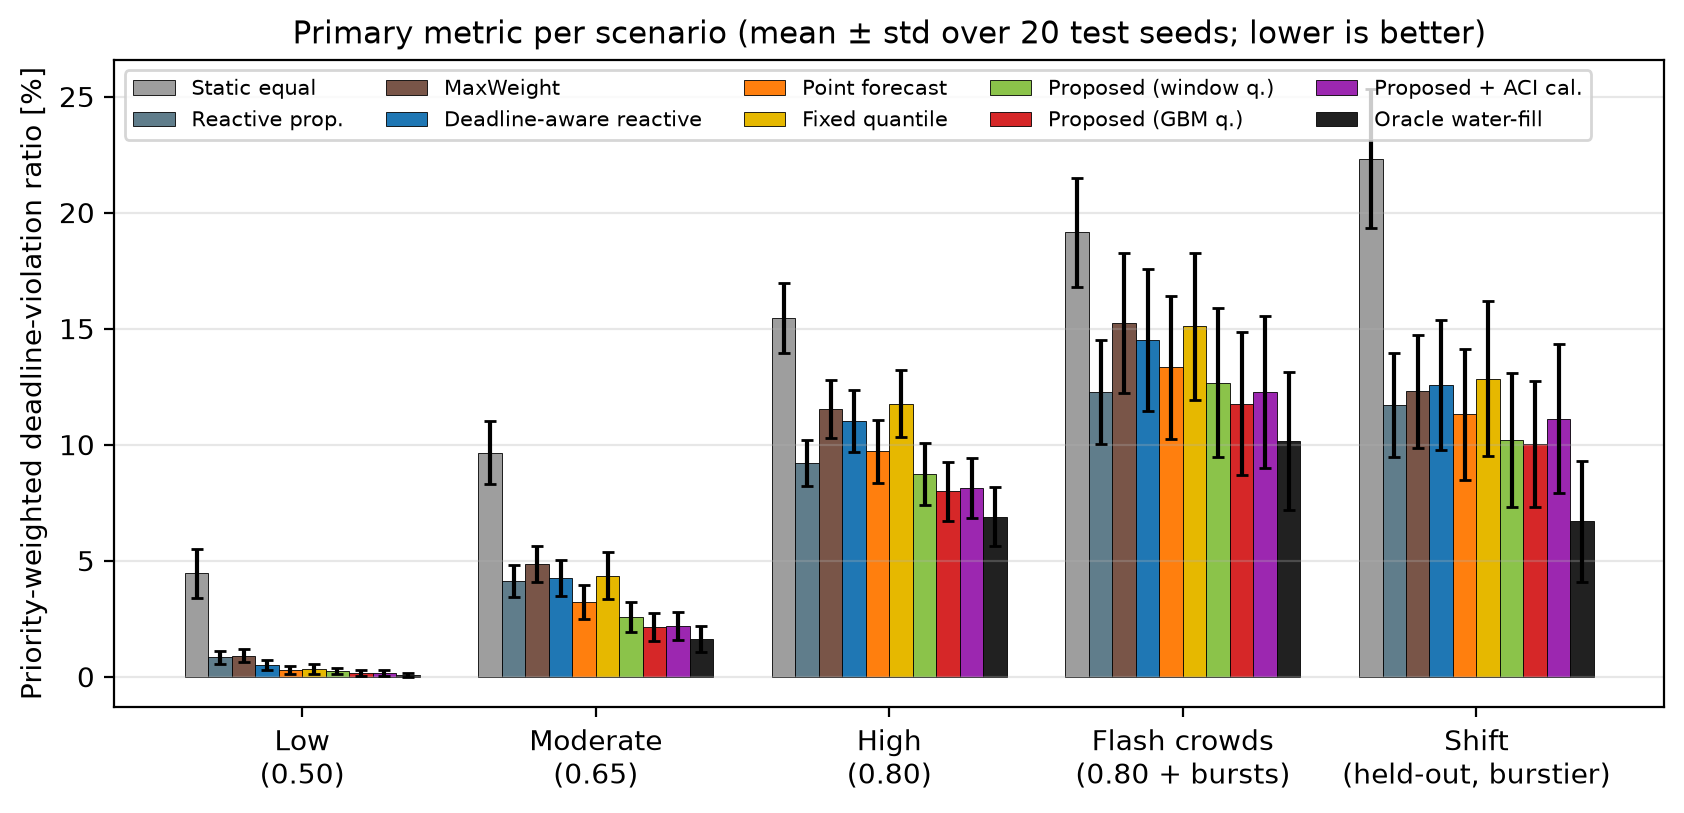
\includegraphics[width=0.9\textwidth]{fig1_primary_by_scenario.png}
\caption{Priority-weighted violation ratio by scenario, Family S; the proposed rule is lowest among implementable controllers everywhere.}
\label{fig:b-main}
\end{figure}

Table~\ref{tab:b-paired} gives the paired reductions per seed. We compared the proposed rule with the point forecast, the fixed quantile, MaxWeight and the deadline-aware reactive controller. It wins against each of them in every scenario, the held-out shift included, on all of the 20 seeds and with $p < 0.01$. Compared with the point forecast it has 11--43\,\% fewer weighted violations. The reduction is 22--54\,\% against the fixed quantile, 19--70\,\% against deadline-aware reactive and 18--83\,\% against MaxWeight. These reductions are plotted in Figure~\ref{fig:b-paired}.

\begin{table}[H]
\caption{Paired per-seed reduction of $V_w$ by the proposed rule, Family S (mean relative change, seeds won out of 20; ** Holm--Wilcoxon $p < 0.01$, * $p < 0.05$).}
\label{tab:b-paired}
\centering\scriptsize
\setlength{\tabcolsep}{4pt}
\begin{tabular}{lccccc}
\toprule
Proposed vs. & low & moderate & high & flash crowds & shift \\
\midrule
Reactive proportional & $-81$\,\% 20/20** & $-48$\,\% 20/20** & $-13$\,\% 20/20** & $-4$\,\% 16/20* & $-14$\,\% 20/20** \\
MaxWeight & $-83$\,\% 20/20** & $-56$\,\% 20/20** & $-31$\,\% 20/20** & $-23$\,\% 20/20** & $-18$\,\% 20/20** \\
Deadline-aware reactive & $-70$\,\% 20/20** & $-49$\,\% 20/20** & $-27$\,\% 20/20** & $-19$\,\% 20/20** & $-20$\,\% 20/20** \\
Point forecast & $-43$\,\% 20/20** & $-33$\,\% 20/20** & $-18$\,\% 20/20** & $-12$\,\% 20/20** & $-11$\,\% 20/20** \\
Fixed global quantile & $-54$\,\% 20/20** & $-50$\,\% 20/20** & $-32$\,\% 20/20** & $-22$\,\% 20/20** & $-22$\,\% 20/20** \\
Window quantiles (no ML) & $-37$\,\% 20/20** & $-16$\,\% 20/20** & $-8$\,\% 20/20** & $-7$\,\% 20/20** & $-2$\,\% 16/20** \\
\bottomrule
\end{tabular}
\end{table}

\begin{figure}[H]
\centering
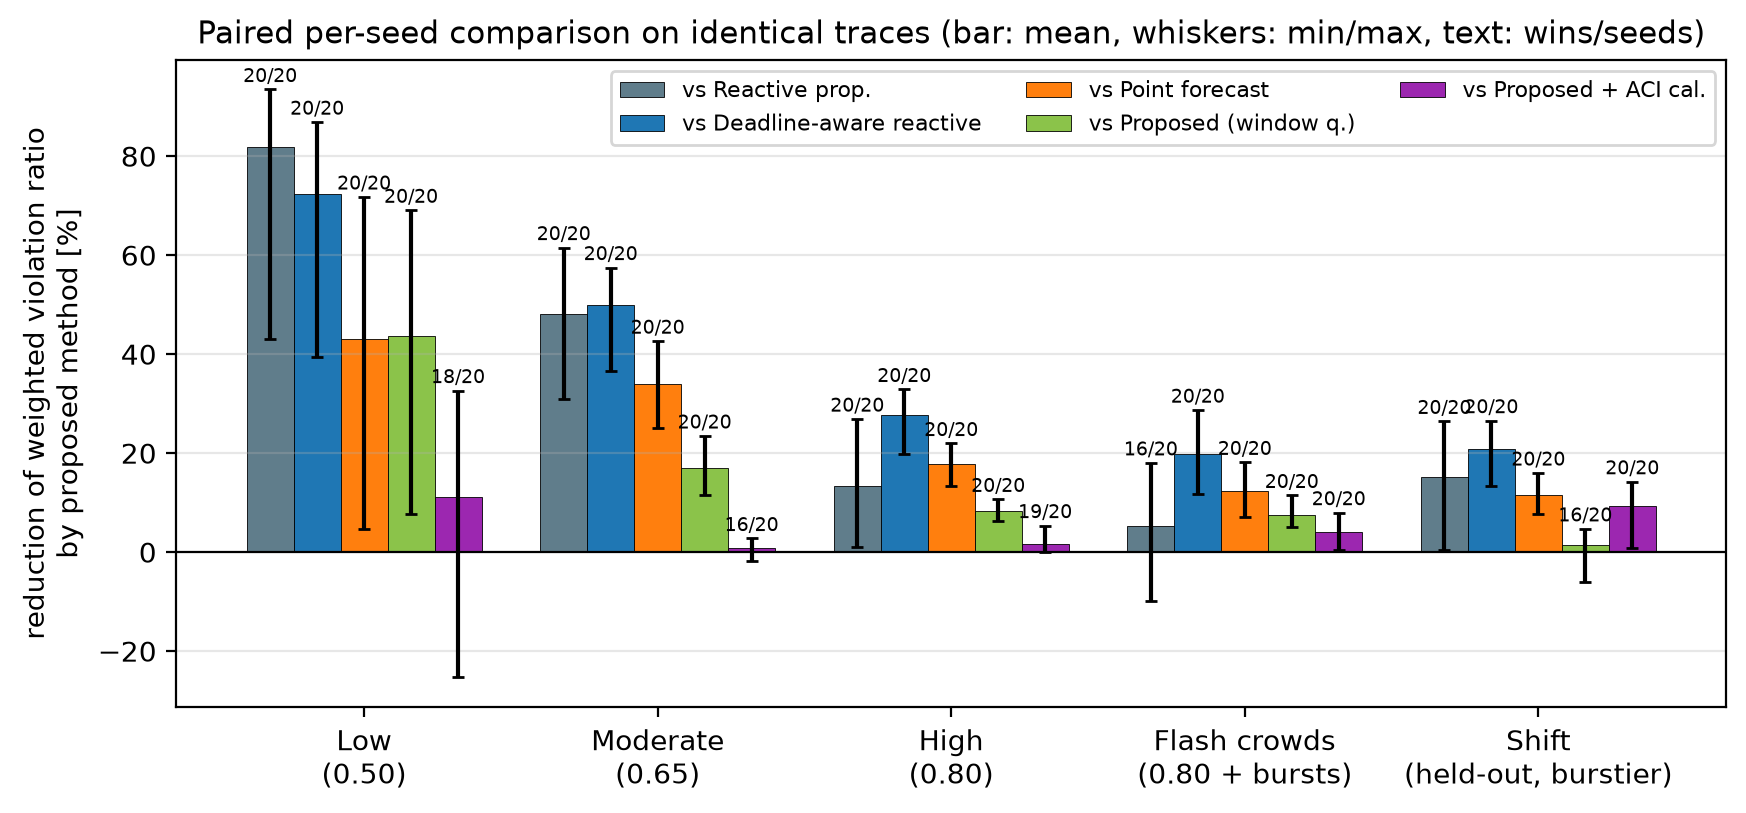
\includegraphics[width=0.85\textwidth]{fig8_paired_reduction.png}
\caption{Paired per-seed reductions of $V_w$ achieved by the proposed rule against each baseline.}
\label{fig:b-paired}
\end{figure}

\section{Where the Gain Comes From}
\label{sec:rb-where}

Table~\ref{tab:b-class} breaks down the high-load result for the deadline-aware controllers. The proposed rule has the lowest eMBB loss (12.3\,\%) and the highest link utilisation (72.2\,\%). This is because it adds margin only where the forecast is wide. A single global quantile level, in contrast, over-protects LL and wastes a third of its allocation. The proposed rule also has the highest Jain fairness (0.997).

\begin{table}[H]
\caption{Deadline-aware controllers, Family S, high load (20 seeds).}
\label{tab:b-class}
\centering\small
\begin{tabular}{lccc}
\toprule
Method & eMBB viol. & Utilisation & Jain \\
\midrule
Deadline-aware reactive & 16.5\,\% & 69.3\,\% & 0.995 \\
Point forecast & 16.0\,\% & 70.1\,\% & 0.994 \\
Fixed global quantile & 22.0\,\% & 67.0\,\% & 0.985 \\
\ours \textbf{Proposed} & \textbf{12.3\,\%} & \textbf{72.2\,\%} & \textbf{0.997} \\
\bottomrule
\end{tabular}
\end{table}

\begin{figure}[H]
\centering
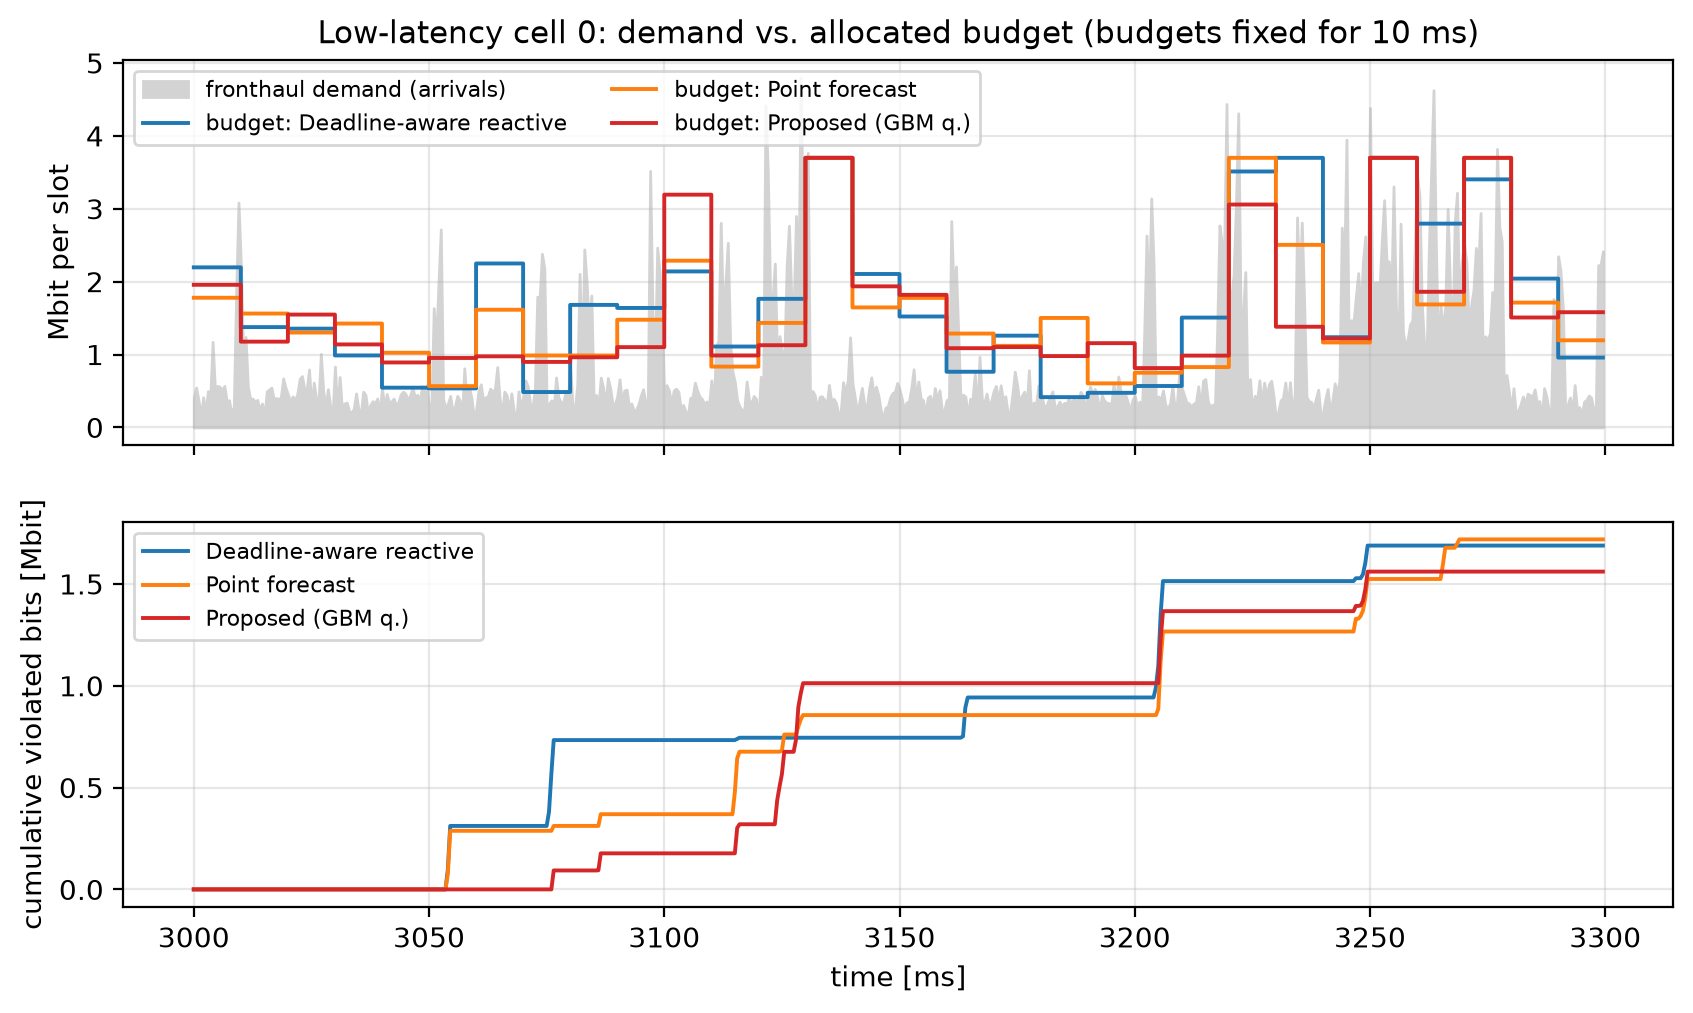
\includegraphics[width=0.7\textwidth]{fig6_demo_timeseries.png}
\caption{The rule in action on one LL cell: grey is demand, steps are budgets held for 10~ms. The reactive controller is one interval late at every burst, while the proposed rule raises the budget at burst onset, where the forecast range is wide, and accumulates the fewest violated bits.}
\label{fig:b-demo}
\end{figure}

\section{Ablations}
\label{sec:rb-abl}

Each ablation below changes one design choice and keeps everything else fixed:
\begin{enumerate}
  \item \textbf{A range versus a single number} (same model, same rule family): $-11$\,\% to $-43$\,\%, with 20/20 seeds in every scenario. This shows that \emph{representing uncertainty matters}.
  \item \textbf{Per-cell KKT level versus one tuned global level} (same forecast): $-22$\,\% to $-54$\,\%. So \emph{the level has to be set per cell by the link constraint}, which is what the KKT rule does.
  \item \textbf{GBM versus window (no-ML) quantiles} under the same KKT rule: GBM adds $-7$\,\% to $-37$\,\% on nominal traffic. Even the no-ML version beats the point forecast in every scenario. The rule itself therefore carries the method, and the learned forecaster improves on it further.
\end{enumerate}

\section{B1 on Family G: Standards-Based 3GPP Traffic}
\label{sec:rb-g}

Table~\ref{tab:b-g} and Figure~\ref{fig:b-g} show that the result carries over to traffic we did not design ourselves. The proposed rule is the best implementable controller at both loads, on 20/20 seeds. At high load it is 11\,\% better than the point forecast, 31\,\% better than deadline-aware reactive and 50\,\% better than reactive proportional. On this family our rule is also the best under the \emph{unweighted} violation ratio (14.3--14.4\,\% for the two variants). A forecaster trained on Family~S and used here without retraining still beats every reactive controller.

\begin{table}[H]
\caption{Family G (3GPP): $V_w$ [\%] at moderate and high load, and the unweighted ratio at high load.}
\label{tab:b-g}
\centering\small
\begin{tabular}{lccc}
\toprule
Method & moderate 0.65 & high 0.80 & unweighted (high) \\
\midrule
Static equal & 10.75 & 13.10 & 19.2 \\
Reactive proportional & 12.05 & 15.94 & 15.0 \\
MaxWeight & 17.51 & 25.79 & 19.7 \\
Deadline-aware reactive & 8.95 & 11.53 & 18.5 \\
Point forecast & 6.00 & 8.98 & 16.6 \\
Fixed quantile & 6.80 & 9.88 & 18.7 \\
Window quantiles & 6.18 & 9.01 & 16.0 \\
\ours \textbf{Proposed} & \textbf{5.08} & \textbf{8.01} & \textbf{14.4} \\
Transfer (trained on S) & 6.99 & 9.89 & 14.3 \\
\midrule
\textcolor{gray}{Oracle + KKT} & \textcolor{gray}{3.47} & \textcolor{gray}{6.06} & \textcolor{gray}{11.1} \\
\bottomrule
\end{tabular}
\end{table}

\begin{figure}[H]
\centering
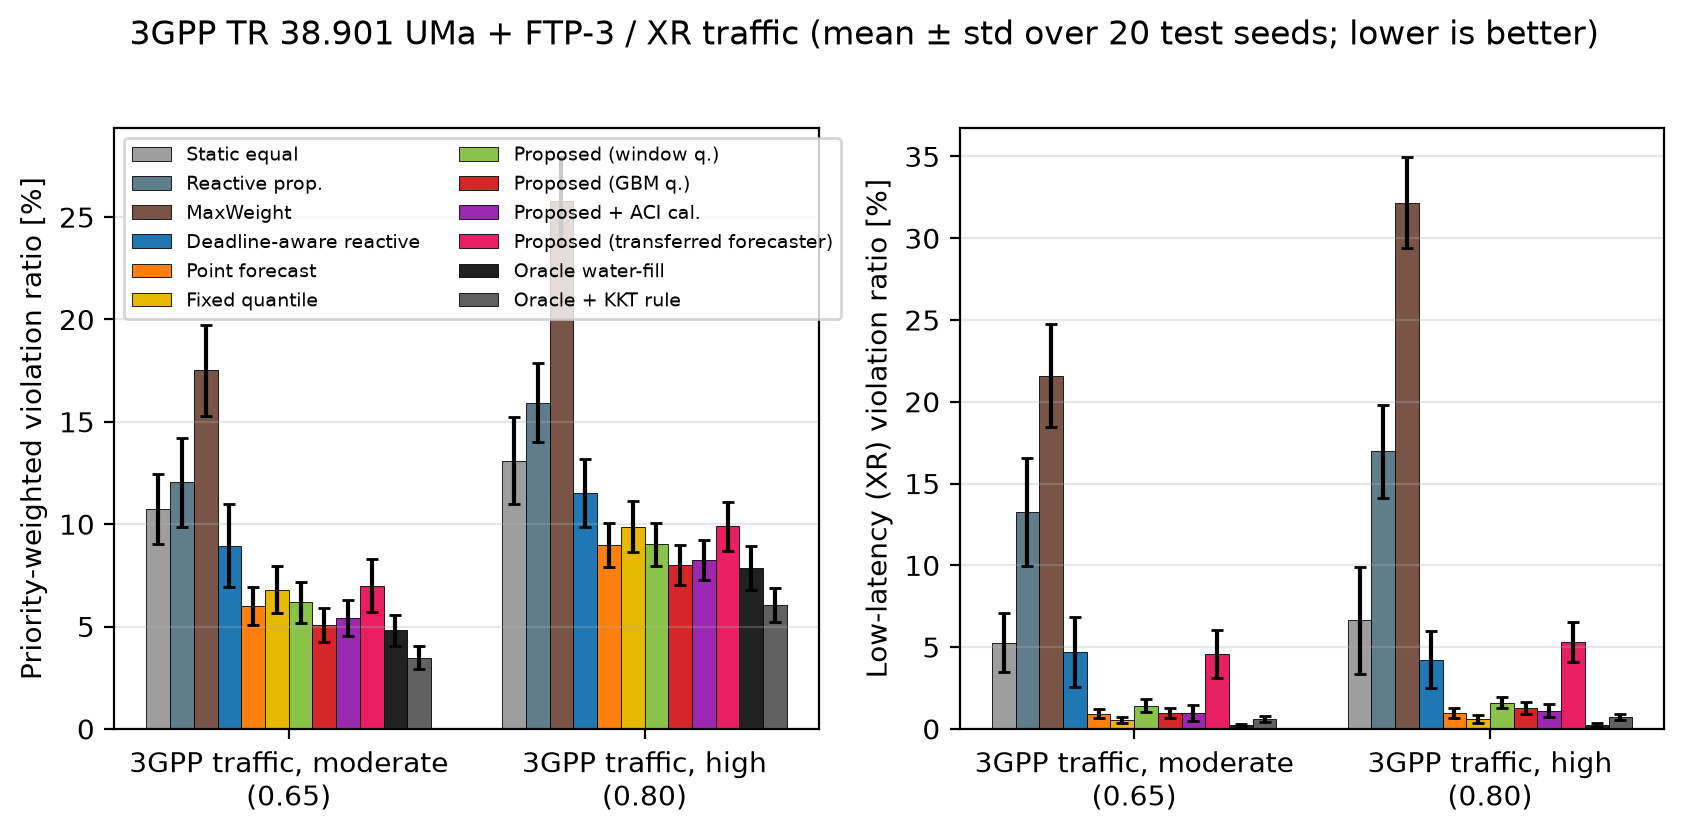
\includegraphics[width=0.8\textwidth]{fig12_tgpp.png}
\caption{Family G (3GPP UMa, FTP Model~3 and XR traffic): the proposed rule leads at both loads.}
\label{fig:b-g}
\end{figure}

\section{Forecast Quality, Robustness and Operating Regime}
\label{sec:rb-robust}

\paragraph{Forecast calibration.} On validation data the GBM quantiles cover 5.6 / 25.6 / 50.7 / 75.3 / 89.9 / 94.9\,\% at nominal levels 5 / 25 / 50 / 75 / 90 / 95\,\%, which means the forecaster is calibrated to within about one percentage point. Its pinball loss is 0.0224, compared with 0.0293 for a window median (Figure~\ref{fig:b-fq}).

\begin{figure}[H]
\centering
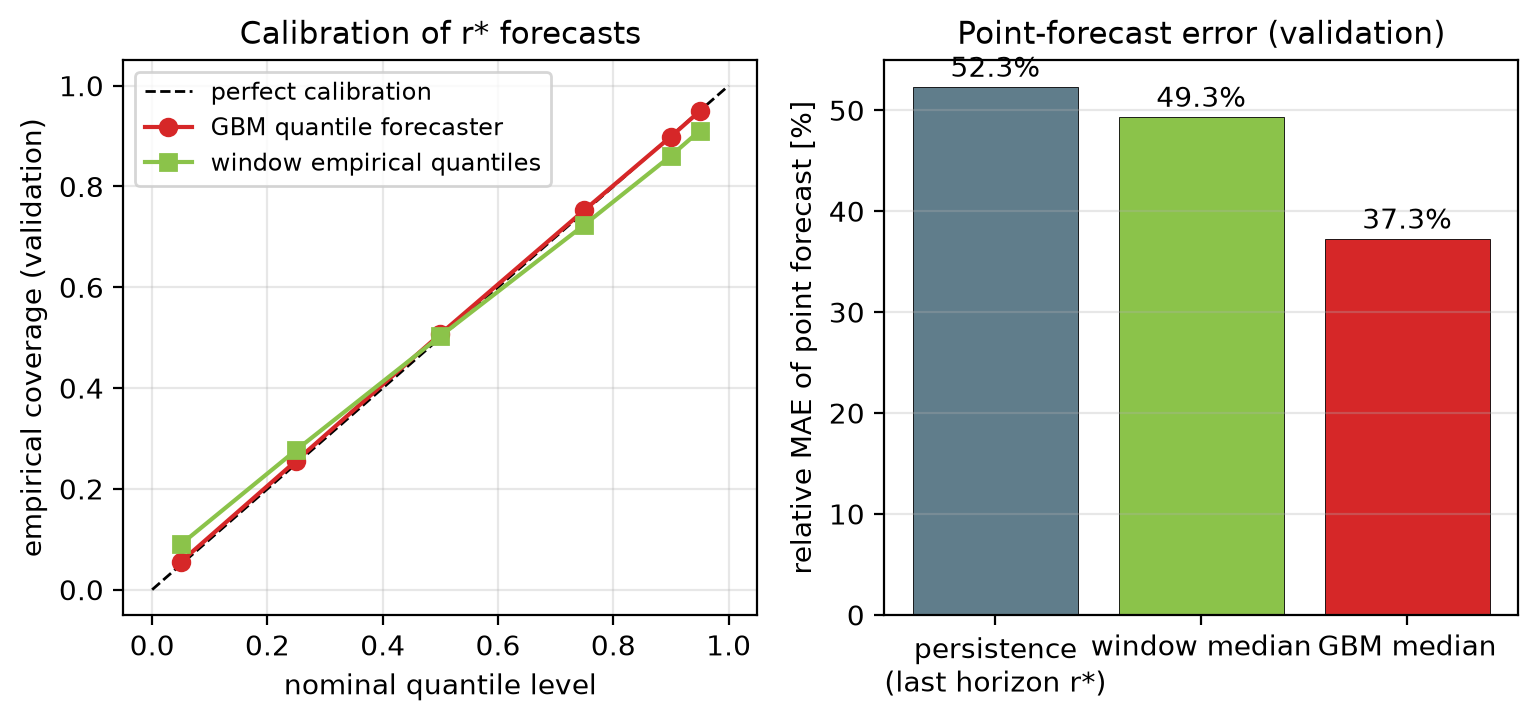
\includegraphics[width=0.62\textwidth]{fig5_forecast_quality.png}
\caption{Calibration of the GBM quantile forecaster on validation data.}
\label{fig:b-fq}
\end{figure}

\paragraph{Robustness to miscalibration.} To check Proposition~\ref{prop:robust} in practice, we shifted every forecast quantile level by $\epsilon$ before the allocation step (Table~\ref{tab:b-miscal}, Figure~\ref{fig:b-miscal}). Under-reserving does almost no harm, because the price $\lambda$ absorbs a common shift. Over-reserving makes things worse, but only gradually. Even at $\epsilon = 0.3$ the rule still matches the point forecast (9.46\,\%) and beats deadline-aware reactive (10.78\,\%).

\begin{table}[H]
\caption{$V_w$ [\%] when every quantile level is shifted by $\epsilon$ (10 seeds).}
\label{tab:b-miscal}
\centering
\begin{tabular}{lccccc}
\toprule
$\epsilon$ & $-0.3$ & $-0.1$ & 0 & $+0.1$ & $+0.3$ \\
\midrule
high & 7.80 & 7.61 & 7.71 & 8.13 & 9.45 \\
shift & 10.96 & 11.10 & 11.13 & 11.53 & 12.50 \\
\bottomrule
\end{tabular}
\end{table}

\begin{figure}[H]
\centering
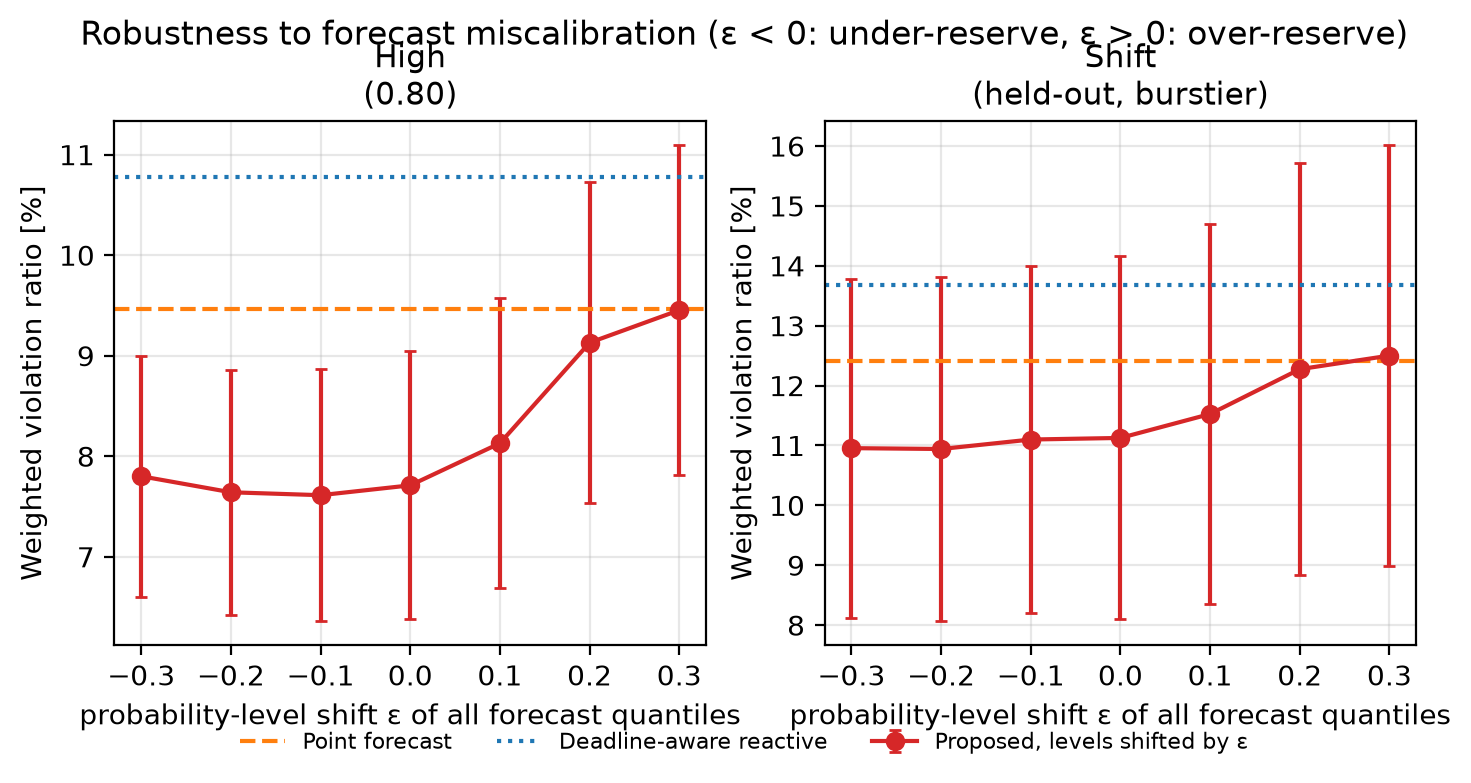
\includegraphics[width=0.6\textwidth]{fig10_miscalibration.png}
\caption{Robustness of the KKT rule to forecast miscalibration.}
\label{fig:b-miscal}
\end{figure}

\paragraph{Control interval and telemetry delay.} Table~\ref{tab:b-interval} varies the control interval and the telemetry delay (10 seeds). The KKT rule is the best controller for every interval from 2 to 10~ms, which is the operating range of a near-RT RIC. At $T = 2$~ms it even beats the oracle water-fill. The advantage is largest when telemetry is fresh ($-16$\,\% against reactive proportional at $\tau = 0$).

\begin{table}[H]
\caption{Sensitivity to control interval $T$ and telemetry delay $\tau$, Family S high load, $V_w$ [\%].}
\label{tab:b-interval}
\centering\small
\begin{tabular}{lccc}
\toprule
$T$ & Reactive prop. & Point forecast & \textbf{Proposed} \\
\midrule
2~ms & 3.91 & 6.57 & \textbf{3.07} \\
5~ms & 7.42 & 7.53 & \textbf{5.07} \\
10~ms & 8.91 & 9.46 & \textbf{7.71} \\
\midrule
$\tau$ & & & vs.\ reactive prop. \\
\midrule
0~ms & 8.16 & 8.45 & \textbf{6.85} ($-16$\,\%) \\
1~ms & 8.91 & 9.46 & \textbf{7.71} ($-13$\,\%) \\
2.5~ms & 9.86 & 10.51 & \textbf{8.77} ($-11$\,\%) \\
5~ms & 11.30 & 12.45 & \textbf{11.07} ($-2$\,\%) \\
\bottomrule
\end{tabular}
\end{table}

\paragraph{Priority weight.} The rule makes use of the operator's priority setting. When the LL weight is raised from 3 to 5, its $V_w$ at high load drops from 8.00 to 6.93\,\%, while that of reactive proportional grows from 9.20 to 10.56\,\%. So the more weight an operator puts on low-latency traffic, the larger the advantage of the proposed rule becomes.

\section{Part A $\times$ Part B: Compression Width and Allocation}
\label{sec:rb-ab}

The two parts of the project meet in the term $\beta(b)$ of Eq.~\eqref{eq:beta}. In Table~\ref{tab:b-ab} the user traffic is kept fixed and only the BFP width is changed. Compression determines the load regime, and allocation determines the loss within that regime. Moving from 9- to 6-bit mantissas lowers the load from 0.65 to 0.44. At 0.65 load the proposed rule cuts the loss of reactive proportional by half (1.96 vs 3.90\,\%). Part~A therefore keeps the link in the operating range where the Part~B allocation rule works best, and this is why the two parts belong together.

\begin{table}[H]
\caption{Compression width versus allocation rule (same user traffic), $V_w$ [\%].}
\label{tab:b-ab}
\centering
\begin{tabular}{lcccc}
\toprule
BFP width & offered load & Reactive prop. & Point forecast & \textbf{Proposed} \\
\midrule
6 bit & 0.44 & 0.22 & 0.15 & \textbf{0.11} \\
9 bit & 0.65 & 3.90 & 3.00 & \textbf{1.96} \\
\bottomrule
\end{tabular}
\end{table}


\section{Decision Overhead}
\label{sec:rb-overhead}

Figure~\ref{fig:b-time} shows the decision time per 10~ms epoch, measured in Python on a 4-core CPU. The KKT rule alone needs less than 0.1~ms. The complete proposed controller, which computes 28 features per cell and evaluates $6\times300$ trees, needs 3.5~ms. This is well inside the 10~ms interval. We also wrote a vectorised numpy tree traversal, and it runs 6.7$\times$ faster than scikit-learn's \texttt{predict} (1.8 vs 12~ms).

\begin{figure}[H]
\centering
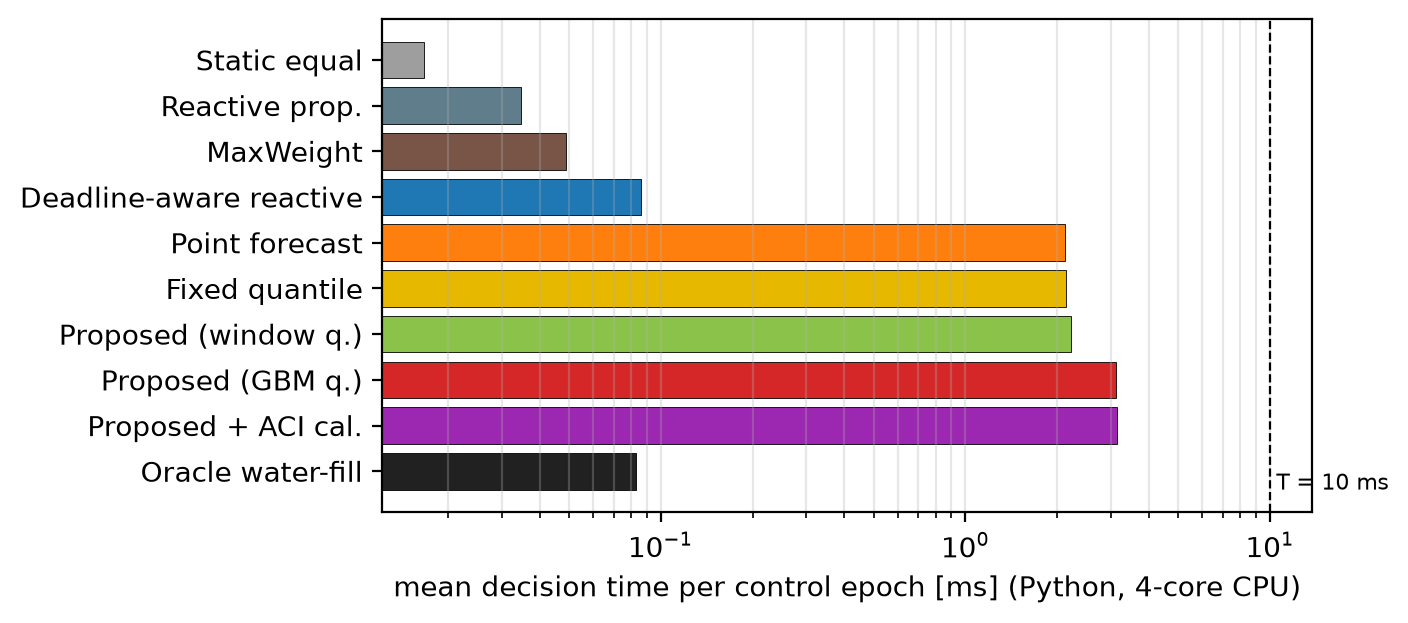
\includegraphics[width=0.62\textwidth]{fig7_decision_time.png}
\caption{Decision time per control epoch (Python, 4-core CPU).}
\label{fig:b-time}
\end{figure}

\section{Extended Study Results}
\label{sec:rb-ext}

Table~\ref{tab:b-ext} compares the best controllers of the extended study over all ten scenarios of the three families, and Figure~\ref{fig:b-ext} shows all 19 controllers. Within the NCC comparison set the KKT rule wins all 10 scenarios, and it is the best controller that has nothing to tune. A Markov chain fitted online, without any training data, comes within 3--9\,\% of the learned rule. Two controllers from the queueing and policy-search literature do better while using the \emph{same} forecaster. The CEM policy is best in 6 of 10 scenarios and predictive MaxWeight in 3, all of them on bursty Family~S. These two are the strongest baselines of the project, and B3 beats both of them.

\begin{table}[H]
\caption{Extended study: $V_w$ [\%] of the strongest controllers across three families.}
\label{tab:b-ext}
\centering\small
\setlength{\tabcolsep}{4pt}
\begin{tabular}{lccccc}
\toprule
Scenario & \makecell{GBM +\\KKT} & \makecell{Pred.\\MaxWeight} & \makecell{CEM\\policy} & \makecell{Markov-\\chain KKT} & \makecell{Tuned-$w$\\KKT} \\
\midrule
S low 0.50 & 0.15 & 0.14 & 0.13 & 0.25 & 0.18 \\
S moderate 0.65 & 2.15 & 1.62 & 1.77 & 2.65 & 2.21 \\
S high 0.80 & 8.00 & 6.15 & 6.57 & 8.64 & 7.88 \\
S flash crowd & 11.76 & 9.69 & 10.20 & 12.44 & 11.49 \\
S shift & 10.04 & 10.25 & 9.73 & 10.22 & 9.90 \\
G moderate 0.65 & 5.08 & 7.57 & 4.58 & 6.44 & 4.98 \\
G high 0.80 & 8.01 & 11.36 & 7.17 & 8.77 & 7.83 \\
M moderate 0.65 & 0.92 & 1.64 & 0.88 & 1.24 & 0.85 \\
M high 0.80 & 4.94 & 4.79 & 3.93 & 5.12 & 4.88 \\
M shift 0.80 & 5.52 & 4.80 & 4.17 & 5.39 & 5.31 \\
\bottomrule
\end{tabular}
\end{table}

\begin{figure}[H]
\centering
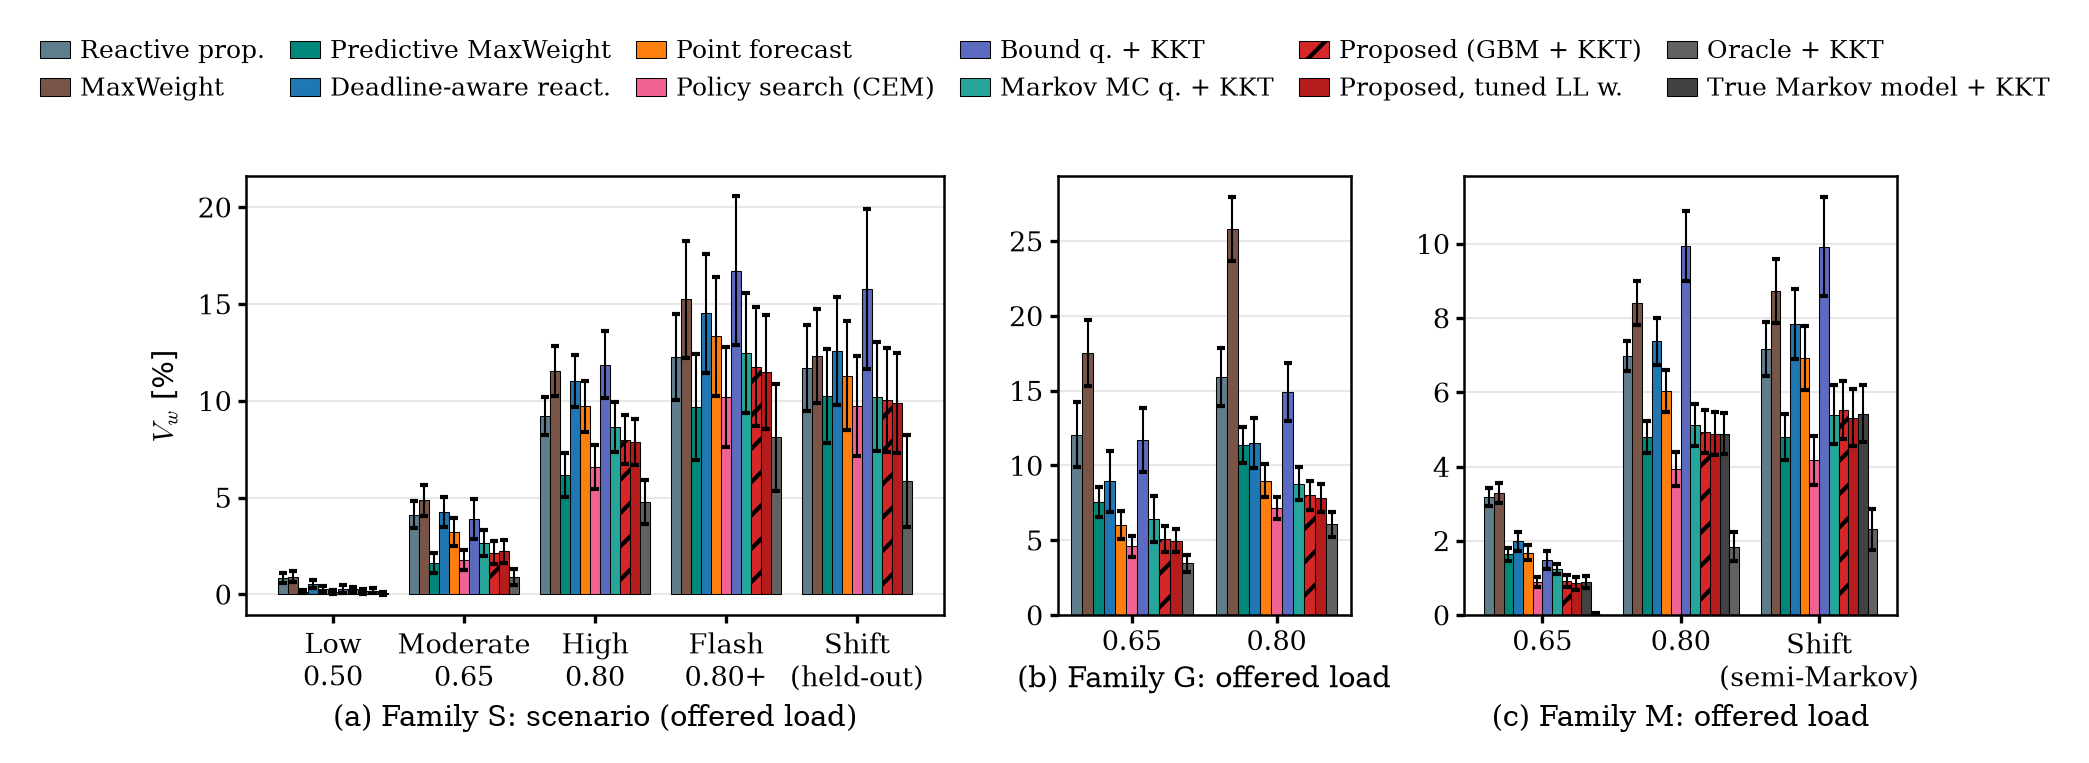
\includegraphics[width=\textwidth]{paper_fig_overview_ext.png}
\caption{All 19 controllers of the extended study on the three traffic families.}
\label{fig:b-ext}
\end{figure}

Looking at the KKT multiplier explains why the remaining gap has this shape. At high load the link is binding in 99.8--100\,\% of epochs, and $\lambda^\ast \ge w_{\rm eMBB}$ holds in 50--58\,\% of them. In half the epochs, then, every eMBB cell is already at its lowest quantile, and re-tuning the LL weight gains only 1--4\,\%. The CEM policy gains for a different reason, namely its \emph{decoupled} per-class levels and a different sharing rule. The gap comes from the structure of the rule and cannot be closed by changing a constant. Figure~\ref{fig:b-regime} maps out the operating regimes. Reservation wins for short intervals and for long bursts (FTP files, XR frames), while back-pressure wins for short bursts at 10--20~ms intervals. In Figure~\ref{fig:b-theory} the Markov-fluid theory is checked against simulation. The shortfall sandwich is never violated and the Chernoff bound holds.

\begin{figure}[H]
\centering
\begin{subfigure}{0.48\textwidth}
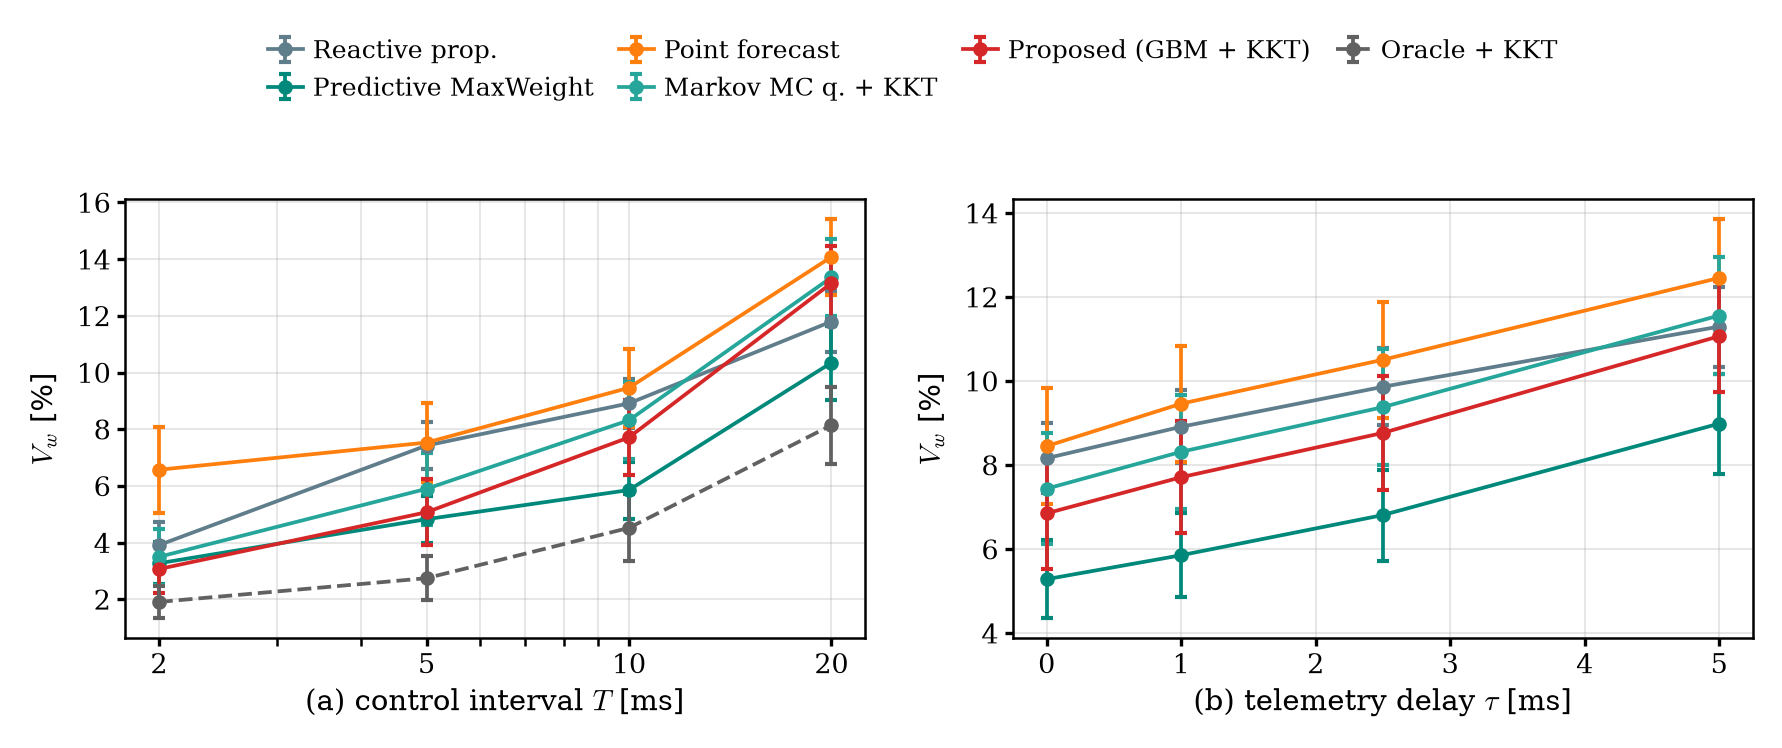
\includegraphics[width=\linewidth]{paper_fig_regime.png}
\caption{Operating regime.}
\label{fig:b-regime}
\end{subfigure}\hfill
\begin{subfigure}{0.5\textwidth}
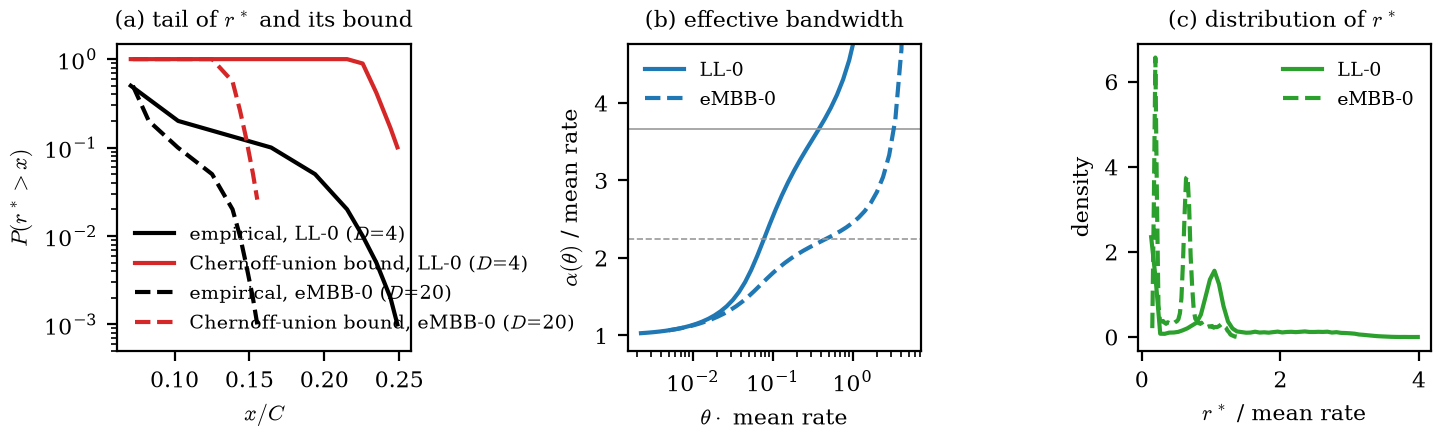
\includegraphics[width=\linewidth]{paper_fig_theory.png}
\caption{Markov-fluid bounds versus simulation.}
\label{fig:b-theory}
\end{subfigure}
\caption{(a) Which structure wins where: reservation versus back-pressure. (b) Validation of the Markov-fluid theory of $\rstar$ on Family~M.}
\end{figure}

\section{B2 Results: the Bayesian Transformer Forecaster}
\label{sec:rb-b2}

\subsection{Forecast quality}

Table~\ref{tab:b2-fq} evaluates all forecasters on the same validation rows and on the held-out shift. Compared with the GBM, the Transformer lowers the pinball loss by 4.5\,\% and the width of the 90\,\% interval by 8\,\%, and its coverage is still higher. The Bayesian ensemble $\times$ MC-dropout mixture is the best calibrated of all models. It has the highest 90\,\% coverage both in distribution (0.919) and under shift (0.808), as well as the best LL upper-tail coverage under shift (0.873).

\begin{table}[H]
\caption{Forecast quality on identical validation rows; ``shift'' is the held-out out-of-distribution test.}
\label{tab:b2-fq}
\centering\scriptsize
\setlength{\tabcolsep}{4pt}
\begin{tabular}{lcccccc}
\toprule
& \multicolumn{4}{c}{Validation (in distribution)} & \multicolumn{2}{c}{Shift (held out)} \\
\cmidrule(lr){2-5}\cmidrule(lr){6-7}
Model & Pinball & Pinball LL & 90\,\% cov. & 90\,\% width & 90\,\% cov. & LL $q_{0.95}$ cov. \\
\midrule
GBM (B1) & 0.0224 & 0.0259 & 0.894 & 1.51 & n/a & n/a \\
LCQT & \textbf{0.0214} & \textbf{0.0251} & 0.902 & \textbf{1.36} & 0.795 & 0.855 \\
\quad without cross-cell layer & 0.0213 & 0.0249 & 0.903 & 1.38 & & \\
\quad unweighted pinball & 0.0213 & 0.0250 & 0.922 & 1.38 & & \\
LCQT + MC dropout (16) & 0.0214 & 0.0251 & 0.911 & 1.41 & 0.802 & 0.870 \\
Deep ensemble (3) & \textbf{0.0212} & \textbf{0.0248} & 0.912 & 1.37 & 0.806 & 0.864 \\
\ours \textbf{Ensemble $\times$ MC (3$\times$8)} & 0.0213 & 0.0249 & \textbf{0.919} & 1.40 & \textbf{0.808} & \textbf{0.873} \\
DF-LCQT (decision-focused) & 0.0224 & 0.0273 & 0.907 & 1.38 & 0.830 & 0.822 \\
\bottomrule
\end{tabular}
\end{table}

\subsection{Closed-loop results}

Table~\ref{tab:b2-cl} gives the closed-loop results on Family~S, with the same traces and seeds in every row. We re-ran the GBM rows, and they match the stored runs exactly because the simulator is deterministic. The Bayesian LCQT is the best variant of the KKT rule, with 0.12 / 2.02 / 7.89\,\% at low / moderate / high load. In the paired comparison with GBM + KKT (Table~\ref{tab:b2-paired}) it improves on the proposed method on every one of the 20 seeds at low, moderate and high load ($-20.8$\,\%, $-6.1$\,\%, $-1.4$\,\%). The main gain comes from the patch Transformer, and the Bayesian mixture adds a consistent further gain.

\begin{table}[H]
\caption{B2 closed loop, Family S: $V_w$ [\%] (mean of 20 test seeds).}
\label{tab:b2-cl}
\centering\small
\begin{tabular}{lccc}
\toprule
Controller & low & moderate & high \\
\midrule
GBM + KKT (B1) & 0.15 & 2.15 & 8.00 \\
LCQT median + water-fill & 0.25 & 3.14 & 9.76 \\
LCQT + KKT & 0.13 & 2.05 & 7.91 \\
\quad without cross-cell layer & 0.13 & 2.05 & 7.94 \\
\quad unweighted pinball & 0.13 & 2.05 & 7.85 \\
MC-dropout LCQT + KKT & 0.12 & 2.04 & 7.93 \\
\ours \textbf{Bayesian LCQT + KKT} (3$\times$8) & \textbf{0.12} & \textbf{2.02} & 7.89 \\
DF-LCQT + KKT & 0.18 & 2.26 & 7.93 \\
\bottomrule
\end{tabular}
\end{table}

\begin{table}[H]
\caption{Bayesian LCQT + KKT versus GBM + KKT, paired over 20 seeds (95\,\% bootstrap CI, Holm--Wilcoxon).}
\label{tab:b2-paired}
\centering
\begin{tabular}{lcc}
\toprule
Scenario & Reduction of $V_w$ & Seeds won \\
\midrule
low & $\mathbf{-20.8\,\%}$ [16.0, 28.3] & 20/20 \\
moderate & $\mathbf{-6.1\,\%}$ [5.1, 7.0] & 20/20 \\
high & $\mathbf{-1.4\,\%}$ [1.0, 1.8] & 20/20 \\
\bottomrule
\end{tabular}
\end{table}


The B2 study also gave a clear scientific finding. Even with the best forecaster we could build, the KKT rule improves only modestly at high load, and CEM and predictive MaxWeight stay 14--28\,\% lower. The remaining gap is caused by the \emph{decision structure} and not by forecast error. B3 changes this structure and keeps the B2 forecaster.

\section{B3 Results: the Back-Pressure Newsvendor}
\label{sec:rb-b3}

\subsection{Diagnosis}

Table~\ref{tab:b3-diag} breaks down the high-load result of Family~S by class. The KKT rule leaves eMBB short (12.3\,\%) and has the lowest link utilisation (72.2\,\%), because LL capacity that is reserved but not used is lost. Back-pressure controllers waste less. BPN gets the advantages of both approaches. Among the implementable controllers it has the lowest $V_w$ (5.23\,\%), the lowest eMBB violation (4.8--4.9\,\%) and the highest link utilisation (76.1\,\%). Its utilisation is even higher than that of the oracle-informed KKT rule (74.8\,\%).

\begin{table}[H]
\caption{Why BPN wins: per-class breakdown, Family S high load (20 test seeds), all in \%.}
\label{tab:b3-diag}
\centering
\begin{tabular}{lccc}
\toprule
Controller & $V_w$ & eMBB viol. & Link util. \\
\midrule
KKT rule (GBM) & 8.00 & 12.3 & 72.2 \\
CEM class-level & 6.57 & 7.1 & 74.7 \\
Pred.\ MaxWeight (CEM-tuned) & 5.98 & 5.9 & 75.5 \\
\ours \textbf{BPN v1} & \textbf{5.23} & 4.9 & \textbf{76.1} \\
\ours \textbf{BPN v2} & 5.32 & \textbf{4.8} & \textbf{76.1} \\
\bottomrule
\end{tabular}
\end{table}

\subsection{Family S}

Table~\ref{tab:b3-s} compares BPN with both of the strongest baselines, each in its best tuning, for three forecasters. When the forecaster is the same, BPN beats both baselines in every scenario. At high load, BPN with the GBM forecaster reaches 5.23\,\%, while CEM-tuned predictive MaxWeight reaches 5.98\,\% and the re-searched CEM policy 6.58\,\%. This puts BPN within 6--10\,\% of the oracle-informed KKT rule, which knows the true future $\rstar$. The B2 Transformer is also worth more here than it was with the KKT rule. With the Bayesian LCQT forecaster, BPN reaches 5.05\,\% at high load, 8.34\,\% under flash crowds and 8.92\,\% under the held-out shift. These are the best results of the whole project.

\begin{table}[H]
\caption{B3, Family S: $V_w$ [\%] (mean of 20 test seeds).}
\label{tab:b3-s}
\centering\small
\setlength{\tabcolsep}{4pt}
\begin{tabular}{llccccc}
\toprule
Forecaster & Controller & low & moderate & high & flash & shift \\
\midrule
\multirow{6}{*}{GBM} & KKT rule (B1) & 0.15 & 2.15 & 8.00 & 11.76 & 10.04 \\
& Pred.\ MaxWeight (grid-tuned) & 0.14 & 1.62 & 6.15 & 9.69 & 10.25 \\
& Pred.\ MaxWeight (CEM-tuned) & 0.16 & 1.66 & 5.98 & 9.36 & 10.46 \\
& CEM class-level (re-searched) & 0.13 & 1.73 & 6.58 & 10.23 & 9.76 \\
& \cellcolor{good!12}\textbf{BPN v1} (6 param.) & \cellcolor{good!12}0.10 & \cellcolor{good!12}1.21 & \cellcolor{good!12}5.23 & \cellcolor{good!12}8.58 & \cellcolor{good!12}9.23 \\
& \cellcolor{good!12}\textbf{BPN v2} (8 param.) & \cellcolor{good!12}0.10 & \cellcolor{good!12}1.21 & \cellcolor{good!12}5.32 & \cellcolor{good!12}8.70 & \cellcolor{good!12}9.26 \\
\midrule
\multirow{4}{*}{LCQT} & Pred.\ MaxWeight (CEM-tuned) & 0.15 & 1.59 & 5.82 & 9.17 & 10.38 \\
& CEM class-level & 0.12 & 1.69 & 6.49 & 10.12 & 9.70 \\
& \cellcolor{good!12}\textbf{BPN v1} & \cellcolor{good!12}0.08 & \cellcolor{good!12}1.14 & \cellcolor{good!12}5.10 & \cellcolor{good!12}8.38 & \cellcolor{good!12}9.04 \\
& \cellcolor{good!12}\textbf{BPN v2} & \cellcolor{good!12}0.08 & \cellcolor{good!12}1.16 & \cellcolor{good!12}5.25 & \cellcolor{good!12}8.59 & \cellcolor{good!12}9.24 \\
\midrule
\multirow{2}{*}{Bayesian LCQT} & \cellcolor{good!12}\textbf{BPN v1} & \cellcolor{good!12}0.08 & \cellcolor{good!12}\textbf{1.11} & \cellcolor{good!12}\textbf{5.05} & \cellcolor{good!12}\textbf{8.34} & \cellcolor{good!12}\textbf{8.92} \\
& \cellcolor{good!12}\textbf{BPN v2} & \cellcolor{good!12}\textbf{0.07} & \cellcolor{good!12}1.12 & \cellcolor{good!12}5.21 & \cellcolor{good!12}8.55 & \cellcolor{good!12}9.12 \\
\midrule
 & \textcolor{gray}{Oracle + KKT (true $\rstar$)} & \textcolor{gray}{0.05} & \textcolor{gray}{0.88} & \textcolor{gray}{4.77} & \textcolor{gray}{8.10} & \textcolor{gray}{5.84} \\
\bottomrule
\end{tabular}
\end{table}

\subsection{Generalisation to Families G and M}

Table~\ref{tab:b3-gm} repeats the comparison on the 3GPP and Markov families. BPN~v2 is the best controller on G moderate, G high and M high, and one of the BPN variants is best in each of the five scenarios. The difference between the versions matters here. In BPN~v1, stage~1 is always strict back-pressure. It therefore cannot represent reservation, and reservation is what the long 3GPP bursts (FTP files, XR frames) need. BPN~v2 adds the sharing exponent $\eta$, so it contains the reservation policy as well, and it is this version that generalises across all three families. On every family its training cost is lower than that of the best baseline (S 0.0387 vs 0.0436, G 0.0527 vs 0.0555, M 0.0196 vs 0.0226).

\begin{table}[H]
\caption{B3 on Families G (3GPP) and M (Markov): $V_w$ [\%], GBM forecaster.}
\label{tab:b3-gm}
\centering\small
\begin{tabular}{lccccc}
\toprule
Controller & G moderate & G high & M moderate & M high & M shift \\
\midrule
KKT rule (B1) & 5.08 & 8.01 & 0.92 & 4.94 & 5.52 \\
Pred.\ MaxWeight (CEM-tuned) & 6.75 & 10.02 & 1.61 & 4.82 & 4.82 \\
CEM class-level (extended study) & 4.58 & 7.17 & 0.88 & 3.93 & 4.17 \\
CEM class-level (re-searched) & 4.51 & 7.05 & 0.94 & 3.94 & 4.22 \\
\ours BPN v1 & 5.67 & 8.92 & \textbf{0.63} & 3.71 & \textbf{3.72} \\
\ours \textbf{BPN v2} & \textbf{4.24} & \textbf{6.81} & 0.68 & \textbf{3.62} & 3.82 \\
\textcolor{gray}{Oracle + KKT} & \textcolor{gray}{3.47} & \textcolor{gray}{6.06} & \textcolor{gray}{0.03} & \textcolor{gray}{1.84} & \textcolor{gray}{2.31} \\
\bottomrule
\end{tabular}
\end{table}

\subsection{BPN v2 against the best baseline in every scenario}

Table~\ref{tab:b3-best} and Figure~\ref{fig:b3-best} give the main result of the project. Here the ``best baseline'' is chosen separately in each scenario as the better of predictive MaxWeight and the CEM class-level policy, each in its own best tuning. BPN~v2 beats this best baseline in all 10 scenarios of all three traffic families, by 3.4\,\% to 25.3\,\%. It wins 20 of 20 seeds in eight scenarios and 19 of 20 at G high, and every comparison is significant after Holm correction ($p \le 0.024$). The grey bars in Figure~\ref{fig:b3-best} show how far behind these baselines the B1 rule was, and how BPN turns that gap into a lead.

\begin{table}[H]
\caption{BPN v2 versus the best baseline in each scenario (paired, 20 test seeds, Holm--Wilcoxon).}
\label{tab:b3-best}
\centering
\begin{tabular}{lcc}
\toprule
Scenario & $V_w$ vs best baseline & Seeds won \\
\midrule
S low & $\mathbf{-23.7\,\%}$ & 15/20 \\
S moderate & $\mathbf{-25.3\,\%}$ & 20/20 \\
S high & $\mathbf{-11.0\,\%}$ & 20/20 \\
S flash & $\mathbf{-7.0\,\%}$ & 20/20 \\
S shift & $\mathbf{-4.8\,\%}$ & 20/20 \\
G moderate & $\mathbf{-5.9\,\%}$ & 20/20 \\
G high & $\mathbf{-3.4\,\%}$ & 19/20 \\
M moderate & $\mathbf{-23.3\,\%}$ & 20/20 \\
M high & $\mathbf{-7.9\,\%}$ & 20/20 \\
M shift & $\mathbf{-8.2\,\%}$ & 20/20 \\
\midrule
\multicolumn{3}{c}{\textbf{10/10 scenarios, 3 families, all $p \le 0.024$}} \\
\bottomrule
\end{tabular}
\end{table}

\begin{figure}[H]
\centering
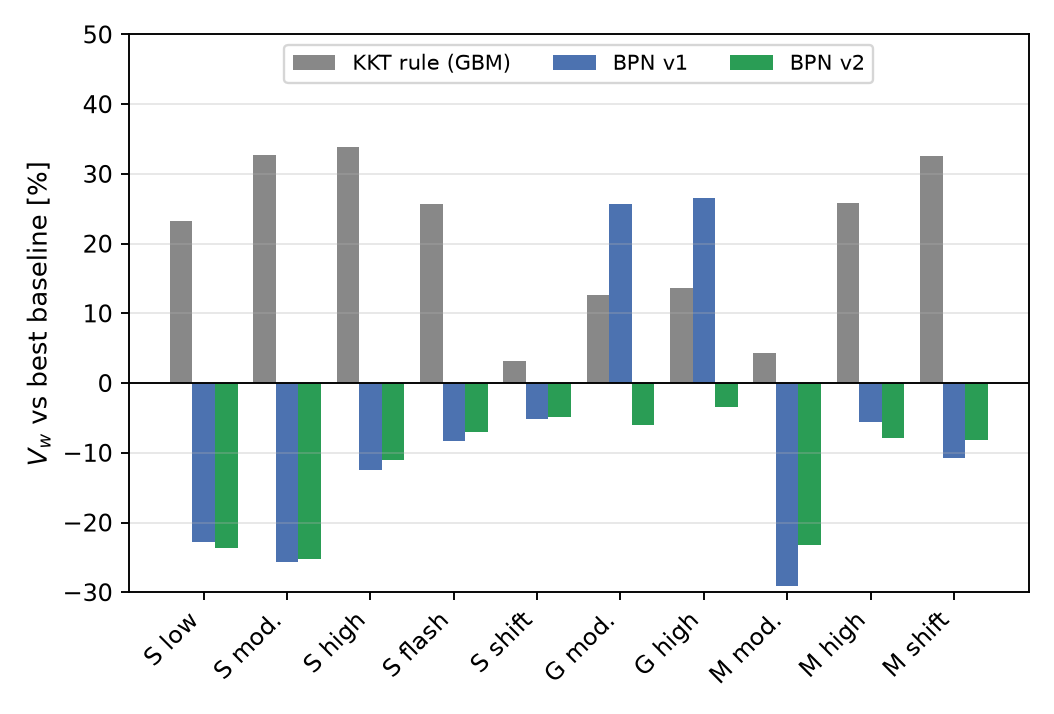
\includegraphics[width=0.8\textwidth]{fig_bpn_vs_best.png}
\caption{Relative $V_w$ against the best baseline in each scenario: the B1 KKT rule (grey), BPN~v1 (blue) and BPN~v2 (green). BPN~v2 is below zero (better than the best baseline) in all ten scenarios.}
\label{fig:b3-best}
\end{figure}

\subsection{What the policy learned}

Since both baselines are special cases of BPN, its learned parameters can be interpreted directly (Table~\ref{tab:b3-theta}). On bursty Family~S the search pushes the sharing exponent to $\eta = 6$, which is strict back-pressure order, with an almost pure drain-rate base ($a = 0.98$). On the 3GPP and Markov families, with their long FTP files and XR frames, it picks $\eta = 0$, which means reservation, together with high LL base quantiles. In this way the search finds the regime map of the extended study by itself, with back-pressure for short bursts and reservation for long ones. BPN is therefore not a black box, because its parameters tell the operator which structure suits the traffic. It takes 2.2--3.5~ms per epoch to decide in Python, which is inside the 10~ms interval.

\begin{table}[H]
\caption{Learned BPN v2 structure per traffic family.}
\label{tab:b3-theta}
\centering
\begin{tabular}{lccc}
\toprule
Family & $\eta$ & $a$ & $(p^0_{\rm LL},\ p^0_{\rm eMBB})$ \\
\midrule
S (bursty) & 6 (strict back-pressure) & 0.98 & (0.41, 0.45) \\
G (3GPP) & 0 (reservation) & 0.31 & (0.94, 0.73) \\
M (Markov) & 0 (reservation) & 0.34 & (0.84, 0.31) \\
R (real 5G traces) & 0.15 (near reservation) & 0.39 & (0.86, 0.28) \\
\bottomrule
\end{tabular}
\end{table}

\subsection{Real 5G traffic traces and an overfitting check}
\label{sec:rb-real}

All the families so far are generated. To test BPN on measured traffic we built a fourth family, R, driven by traces from a public 5G dataset of a commercial Irish operator~\cite{raca2020beyond}. The dataset contains 166 client-side sessions of Netflix and Amazon Prime streaming and of file download, both static and while driving, with downlink throughput and CQI logged about once per second. Each cell aggregates six sessions started at random offsets. The cost of each user is its measured rate divided by the spectral efficiency of its measured CQI (from the LTE CQI table), so the traffic and the per-cell fronthaul cost per bit both come from the measurements. Each one-second sample is replayed for one 10~ms control interval. This keeps the real sequence of rates but compresses time by 100$\times$, and it has two consequences. First, the rate changes between consecutive intervals by as much as it really changes in one second. The forecaster's task is therefore harder than it would be with real timing, where a cell's rate is nearly constant over 100 intervals and the last value would be an excellent forecast. Second, the one-second samples contain no bursts on the millisecond scale. Family R thus tests how controllers deal with measured session-level structure (application mix, mobility, CQI) rather than packet-level burstiness, which families S, G and M already cover. So family R is a stress test of the slow dynamics and not a replay of real fronthaul timing. Cells are scaled to the scenario load using the LL / eMBB shares of the other families, and they are clipped at their own air-interface peak. The sessions are split only once. Two thirds are used to train the GBM forecaster and to run the policy searches, and the test seeds draw only from the remaining third, so no test session is ever seen in training.

BPN v2 tunes 8 parameters, so a large lead might simply come from fitting the search episodes. To check this we re-ran every CEM search on family R twice, for BPN v2 and for both strongest baselines. One run used the usual 8 search episodes and the other used only 2. All controllers were then tested on the same 20 test seeds (Table~\ref{tab:b3-real}).

\begin{table}[H]
\caption{Family R (real 5G traces): $V_w$ in \% on 20 test seeds from held-out sessions, with each CEM search run on 8 or on 2 episodes.}
\label{tab:b3-real}
\centering
\begin{tabular}{lcc}
\toprule
Controller & R moderate (0.65) & R high (0.80) \\
\midrule
B1 KKT rule (GBM) & 4.20 & 8.79 \\
Predictive MaxWeight, CEM (8 / 2 episodes) & 4.58 / 4.58 & 9.04 / 9.04 \\
Class-level policy, CEM (8 / 2 episodes) & 3.77 / 3.74 & 8.03 / 8.05 \\
\ours \textbf{BPN v2, 8 episodes} & \textbf{3.54} & \textbf{7.47} \\
\ours BPN v2, 2 episodes & 3.74 & 7.80 \\
\midrule
Oracle-informed KKT (reference) & 1.12 & 3.95 \\
\bottomrule
\end{tabular}
\end{table}

On measured traffic BPN v2 is again the best implementable controller. Its $V_w$ is 6.1\,\% and 7.0\,\% lower than that of the best baseline, the class-level policy, at moderate and high load, and it wins 19 and 20 of 20 seeds. Against the B1 rule its $V_w$ is 15--16\,\% lower on 20 of 20 seeds, with Holm--Wilcoxon $p < 0.001$ in every case. The search again picks a near-reservation structure ($\eta = 0.15$), as it did for the long bursts of families G and M (Table~\ref{tab:b3-theta}).

The overfitting check gives the opposite of what overfitting would predict. Had the 8-parameter fit memorised its episodes, the 8-episode BPN would generalise worse than the 2-episode one. It is instead 4--5\,\% \emph{better} on the unseen test sessions and wins 18 of 20 seeds at both loads ($p \le 0.0005$). BPN benefits from more training data, whereas the 2--3-parameter baselines are already saturated and do not change. With only 2 episodes BPN still beats the B1 rule by 11\,\% (19 and 20 of 20 seeds), and it beats the best baseline at high load by 3.1\,\% ($p = 0.04$ after Holm). At moderate load it ties with the best baseline. The gap to the oracle-informed rule is larger on real traffic than on the generated families, because measured streaming traffic is harder to forecast.

\section{Summary}

Table~\ref{tab:b-summary} collects the main results of Part~B. The KKT newsvendor rule (B1) is the best of the 12 reference controllers of the first comparison in every scenario of two traffic families, although the stronger baselines of the extended study beat it. The Bayesian LCQT (B2) improves it on every seed from low to high load and gives the best-calibrated forecasts. The back-pressure newsvendor (B3) is a learned policy that contains both strongest baselines. It beats them in all 10 scenarios of three traffic families, gives the best result of the project at every load, and keeps its lead on measured 5G traffic.

\begin{table}[H]
\caption{Part B headline results.}
\label{tab:b-summary}
\centering\small
\renewcommand{\arraystretch}{1.2}
\begin{tabularx}{\textwidth}{>{\raggedright\arraybackslash}p{4.2cm}>{\raggedright\arraybackslash}X}
\toprule
Step & Headline result \\
\midrule
B1: KKT newsvendor rule & Best of the 12 first-comparison controllers in all scenarios of 2 families; $-11$ to $-43$\,\% vs the forecast median and $-19$ to $-70$\,\% vs deadline-aware reactive, every seed, $p < 0.01$ \\
Ablations & The $\rstar$ target and the per-cell KKT split carry the gain; the learned forecaster adds up to 37\,\% \\
Family G (3GPP) & Result reproduces on standards-based traffic; also best under the unweighted ratio \\
Extended study & POMDP view; $\rstar$ linked to effective bandwidth; KKT rule wins all 10 scenarios of the NCC comparison set \\
B2: Bayesian LCQT & $-4.5$\,\% pinball, best calibration; $-21$ / $-6$ / $-1.4$\,\% $V_w$ at low / moderate / high load, 20/20 seeds \\
\textbf{B3: back-pressure newsvendor} & \textbf{Beats predictive MaxWeight and policy search in 10/10 scenarios of 3 families ($-3$ to $-25$\,\%, $p \le 0.024$)}; within 6--10\,\% of the oracle-informed rule at high load \\
Real 5G traces (family R) & BPN v2 $-6$ / $-7$\,\% vs the best baseline and $-15$\,\% vs B1 on held-out sessions ($p < 0.001$); tuning on fewer episodes makes it worse, not better, so the gain is not overfitting \\
\bottomrule
\end{tabularx}
\end{table}

% =====================================================================
\chapter{Implementation and Experimental Results on Hardware}
\label{ch:impl}
\thispagestyle{plain}
% =====================================================================

\section{Introduction}

A precoder or controller that is accurate in simulation is only useful if it meets the real-time budget of the O-DU. This chapter describes the implementation side of the project: the hand-optimised C/AVX-512/OpenMP kernel that computes the whole RZF precoder of Eq.~\eqref{eq:rzf} for 273 PRBs in a fraction of the 0.5~ms slot (Sections~\ref{sec:hw-platform}--\ref{sec:hw-results}), and the software framework used for every experiment of this report (Section~\ref{sec:sw}).

\section{Hardware Platform}
\label{sec:hw-platform}

All timing measurements were made on a 4-core Intel Xeon server CPU with AVX-512 support, the class of general-purpose processor used in software-defined, cloud-native O-DU deployments. Kernels were compiled with GCC and timed with \texttt{rdtsc} cycle counters for per-stage profiling and with wall-clock time (median of 40 runs) for end-to-end results. The data type is single-precision complex (\texttt{complex64}), as used in O-DU baseband processing; accuracy is always checked against a float64 reference.

\section{Design of the Fused RZF Precoder Kernel}
\label{sec:hw-kernel}

The kernel (\texttt{kernels/cmat\_kernels.c}, Python binding \texttt{cmatinv/fastkernels.py}) is a batched complex64 implementation of $G = HH^H + \alpha I$, $G^{-1}$ and $W = H^H G^{-1}$ for all PRBs of a slot. Figure~\ref{fig:kernel} shows its dataflow. The key design decisions are:

\begin{itemize}
  \item \textbf{One fused pass per PRB.} $H$ is loaded once; Gram, inverse, $W^T$ and power scaling are computed back-to-back on stack and L1-resident buffers, with no DRAM intermediates.
  \item \textbf{Hermitian symmetry.} Only the lower triangle of the Gram matrix is computed.
  \item \textbf{Split real/imaginary planes} (structure of arrays), so that complex arithmetic vectorises cleanly.
  \item \textbf{In-place Gauss--Jordan sweep inverse.} $K$ rank-1 updates on contiguous, fully vectorised rows, without square-root or division chains; no pivoting is needed because $G \succ 0$ (a Cholesky path is kept behind \texttt{-DUSE\_CHOL}).
  \item \textbf{Register-blocked weight formation} $W = H^H X$, with output layout $W^T[S,K,M]$.
  \item \textbf{AVX-512 code generation} (\texttt{-mprefer-vector-width=512}; GCC defaults to 256-bit vectors).
  \item \textbf{OpenMP} \texttt{parallel for} across the 273 PRBs and \texttt{omp simd} inner loops.
  \item \textbf{Fused Newton step} for the RMT-WS warm start, which returns the exact residual $\|I - GX\|_F/\sqrt K$ at no extra cost.
\end{itemize}

\begin{figure}[H]
\centering
\begin{tikzpicture}[font=\footnotesize,>=Stealth,
   s/.style={draw,rounded corners,align=center,minimum height=1.05cm,text width=2.25cm,fill=soft},
   g/.style={s,fill=good!15}]
  \node[s,fill=iitblue!12] (h) {Load $H$\\(re/im planes)};
  \node[s,right=0.45cm of h] (gram) {Gram\\lower triangle\\$HH^H + \alpha I$};
  \node[g,right=0.45cm of gram] (inv) {GJ sweep inverse\\or fused\\Newton step};
  \node[s,right=0.45cm of inv] (w) {$W^T = (H^H G^{-1})^T$\\register-blocked};
  \node[s,right=0.45cm of w,fill=orange!15] (sc) {Power\\scaling\\$\to$ output};
  \draw[->,thick] (h) -- (gram);
  \draw[->,thick] (gram) -- (inv);
  \draw[->,thick] (inv) -- (w);
  \draw[->,thick] (w) -- (sc);
  \node[draw,dashed,rounded corners,fit=(h)(gram)(inv)(w)(sc),inner sep=7pt,label={[font=\footnotesize]below:one PRB, L1-resident, AVX-512 \texttt{omp simd} \qquad $\times$ 273 PRBs in parallel (OpenMP)}] {};
\end{tikzpicture}
\caption{Dataflow of the fused RZF precoder kernel for one PRB; PRBs are processed in parallel across cores.}
\label{fig:kernel}
\end{figure}

The inner loop of the sweep inverse illustrates the style of the kernel: one rank-1 update of all rows except the pivot row, written so that the compiler emits fused multiply-add AVX-512 instructions on the split real and imaginary planes.

\begin{lstlisting}
// inner loop of the in-place Gauss-Jordan sweep inverse (pivot k)
for (int i = 0; i < K; i++) {
  if (i == k) continue;
  float fr = ckr[i]*piv, fi = cki[i]*piv;
  float *ar = xr + i*K, *ai = xi + i*K;
  #pragma omp simd
  for (int j = 0; j < K; j++) {
    ar[j] -= fr*rkr[j] - fi*rki[j];
    ai[j] -= fr*rki[j] + fi*rkr[j];
  }
  ar[k] = -fr; ai[k] = -fi;
}
\end{lstlisting}

The kernel is built with
\begin{lstlisting}[language=bash]
gcc -O3 -march=native -fopenmp -ffast-math \
    -mprefer-vector-width=512 -shared -fPIC cmat_kernels.c -o libcmat.so -lm
\end{lstlisting}

\section{Profiling-Driven Optimisation}
\label{sec:hw-opt}

The kernel was optimised step by step, guided by per-stage cycle counts ($K=16$, $M=64$, one thread):
\begin{enumerate}
  \item \textbf{Fusion and Hermitian symmetry}: the Gram matrix is formed on the lower triangle only, inside the per-PRB pass.
  \item \textbf{Register-blocked weight formation} $W = H^H X$ with output $W^T[S,K,M]$: from 0.81 to \textbf{0.42~ms} per slot.
  \item \textbf{Gauss--Jordan sweep instead of Cholesky}: the inverse drops from 6.4k to \textbf{2.9k cycles} per PRB at $K=16$, and from 21k to 11k cycles at $K=32$.
  \item \textbf{AVX-512 code generation}: 1.3--1.5$\times$ faster on one thread and 2$\times$ on four threads.
  \item A 4-column blocked Gram variant was measured and reverted because it was slower.
\end{enumerate}
After tuning, weight formation takes 44--58\,\% of the cycles at about 30 flops/cycle (about half of the AVX-512 peak), the Gram matrix 20--24\,\% at about 28 flops/cycle, and the inverse the rest.

\section{Experimental Results}
\label{sec:hw-results}

\subsection{Whole precoder per slot}

Table~\ref{tab:hw-pipeline} and Figure~\ref{fig:hw-pipeline} report the time to compute the complete precoder (Gram, inverse and weights) for all 273 PRBs of a slot. \textbf{The fused kernel is 10--15$\times$ faster than numpy + LAPACK.} For $K = 16$ users and $M = 64$ antennas it takes 0.226~ms, less than half of the 0.5~ms slot, where numpy + LAPACK needs 3.21~ms, six times the slot. With the kernel, $K = 8$ and $K = 16$ at $M = 64$, and $K = 16$ at $M = 128$, \textbf{fit the slot for the entire precoder}. None of these configurations did before. Thread scaling is near-linear: 0.92, 0.45 and 0.23~ms on 1, 2 and 4 threads.

\begin{table}[H]
\caption{Whole-precoder time per slot (273 PRBs, complex64, 4-core AVX-512 Xeon, median of 40 runs).}
\label{tab:hw-pipeline}
\centering
\begin{tabular}{lcccc}
\toprule
$K$, $M$ & numpy + LAPACK & Our kernel, 1 thread & \textbf{Our kernel, 4 threads} & Speed-up \\
\midrule
8, 64 & 1.08~ms & 0.268~ms & \textbf{0.070~ms} & 15$\times$ \\
\ours 16, 64 & 3.21~ms & 0.917~ms & \textbf{0.226~ms} & \textbf{14$\times$} \\
32, 64 & 12.2~ms & 3.75~ms & 0.97~ms & 12.5$\times$ \\
16, 128 & 4.71~ms & 1.61~ms & \textbf{0.41~ms} & 11.6$\times$ \\
32, 128 & 16.3~ms & 6.43~ms & 1.60~ms & 10$\times$ \\
\bottomrule
\end{tabular}
\end{table}

\begin{figure}[H]
\centering
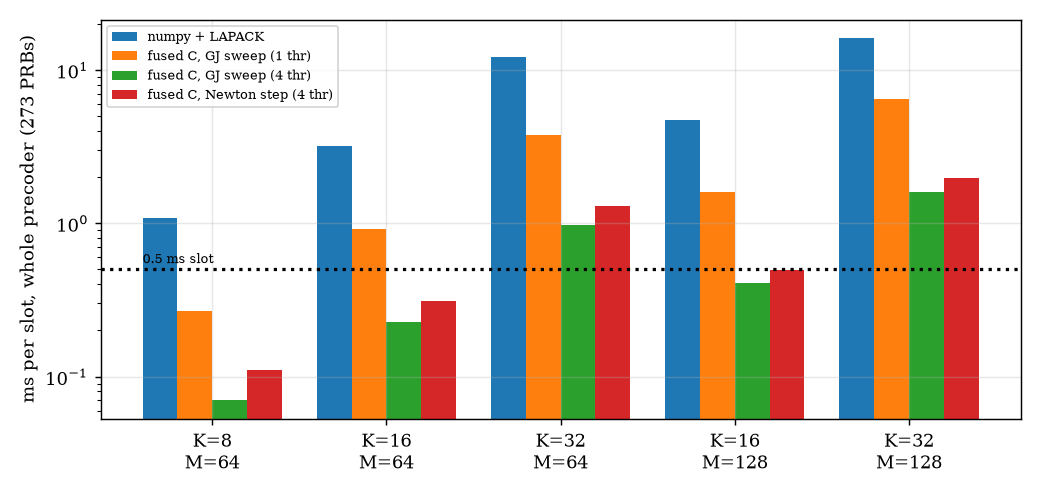
\includegraphics[width=\textwidth]{exp17_pipeline_kernel.png}
\caption{Whole-precoder time per slot; the fused kernels run below the 0.5~ms slot line for $K \le 16$, while numpy + LAPACK never does.}
\label{fig:hw-pipeline}
\end{figure}

\subsection{Inverse kernels}

Figure~\ref{fig:hw-inv} isolates the inverse. The C kernels are an order of magnitude faster than numpy/LAPACK, and the \textbf{fused Newton--Schulz step of RMT-WS is the fastest inverse for $K \le 16$} (0.115~ms per slot at $K=16$, against 0.124~ms for a tuned C Cholesky inverse and 1.6~ms for LAPACK). This is the per-slot warm-start update of Chapter~\ref{ch:parta-methods} running at hardware speed.

\begin{figure}[H]
\centering
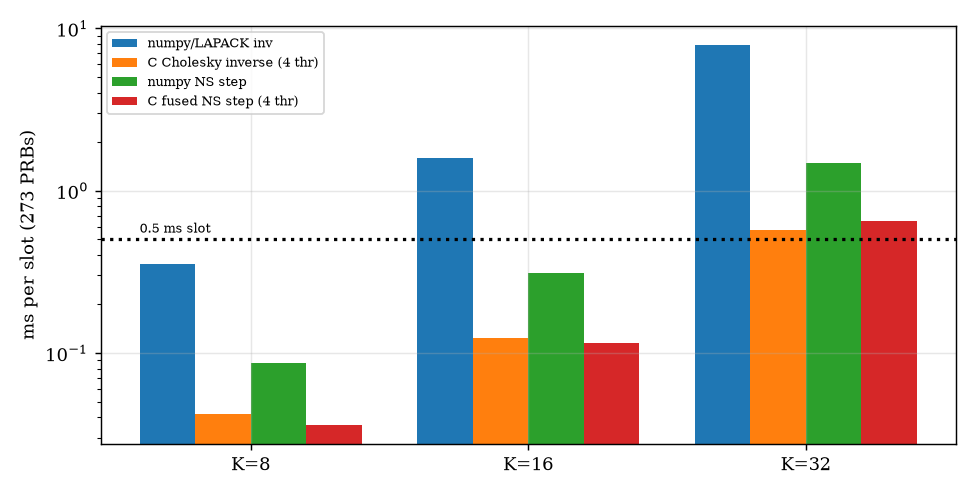
\includegraphics[width=0.85\textwidth]{exp15_kernel_bench.png}
\caption{Inverse-only time per slot (273 PRBs): numpy/LAPACK, tuned C Cholesky, numpy Newton--Schulz step and our fused C Newton--Schulz step (4 threads).}
\label{fig:hw-inv}
\end{figure}

\subsection{Accuracy}

The complex64 kernel reproduces the float64 exact precoder with a sum-rate loss of about $10^{-6}\,\%$ or less in every tested configuration ($K=16$ at 10 and 30~dB, an ill-conditioned 3$^\circ$-spread channel at 25~dB, $K=32$ at 20~dB and $K=16$, $M=128$ at 30~dB). The speed-up therefore comes at no cost in link performance.

\section{Software Framework and Reproducibility}
\label{sec:sw}

All results of this report are produced by an open, fully reproducible Python/C code base (Table~\ref{tab:repo}). The Part~B simulator is slot-accurate: it generates the three traffic families, applies the stale observations and the held budgets, runs FIFO queues with deadline drops for every cell and records every metric. Every number in our papers is generated as a macro from the result CSV files, so text and data cannot diverge.

\begin{table}[H]
\caption{Structure of the project repository.}
\label{tab:repo}
\centering\small
\begin{tabularx}{\textwidth}{>{\ttfamily}p{4.4cm}X}
\toprule
\normalfont Module & Content \\
\midrule
matinv\_bench/ & inversion benchmark, InverseNet-MLP/NS/Ultra \\
cmatinv/, experiments\_v2/ & complex inversion, RMT-WS, 38.901 channels, Experiments 5--18 \\
kernels/ & fused C/AVX-512/OpenMP precoder kernel \\
experiments/ & Part~A Experiments 1--4, extended Part~B pipeline \\
fhlm/ & Part~B simulator, traffic families S, G, M, forecasters, 19+ controllers, theory, figures, tables \\
fhlm/transformer.py, decision\_focused.py & B2: LCQT, Bayesian mixture, differentiable KKT layer \\
fhlm/hybrid.py & B3: back-pressure newsvendor and equal-budget CEM search \\
tests/ & 46 unit tests: capacity in every slot, no future leakage, bound validity, KKT-layer gradients, policy containment \\
results/ & all CSV files, logs and figures \\
\bottomrule
\end{tabularx}
\end{table}

\paragraph{Verification.} The unit tests check, among other properties, that the link capacity is respected in every slot, that no feature uses future data, that the deadline-feasible rate is tight, that the theoretical bounds hold, that the differentiable KKT layer matches the numpy allocator to $10^{-6}$ with correct gradients, and that BPN reproduces predictive MaxWeight and the CEM policy exactly with the corresponding parameters.

\section{Discussion and Analysis}

This chapter discussed the hardware results of the project. The fused C/AVX-512/OpenMP kernel turns the RZF precoder from a computation that is six times too slow for the slot into one that uses less than half of it, with float64-level accuracy. This is what makes per-slot RU-side precoding, with its 72\,\% fronthaul saving, practical on a general-purpose CPU O-DU. On the Part~B side, every controller runs well within its 10~ms decision interval in Python (3.5~ms for the KKT rule with GBM, 2.2--3.5~ms for BPN), and the fully tested, reproducible framework makes every result of this report traceable to its data.

% =====================================================================
\chapter{Conclusions and Scope for Future Work}
\label{ch:concl}
\thispagestyle{plain}
% =====================================================================

\section{Conclusions}

This project set out to make the O-RAN fronthaul both \emph{lighter} and \emph{smarter}. It delivered a complete, end-to-end solution: Part~A reduces the bits that cross every fronthaul link, and Part~B decides, ahead of time and under uncertainty, how the remaining capacity of a shared link is divided among the cells. Both parts are backed by theorems, by large statistically tested experiments and by a fully reproducible code base.

\subsection*{Part A: lighter fronthaul and real-time precoding}
\begin{itemize}
  \item \textbf{Channel compression.} CSEE and RAS-BFP compress reference-symbol and channel IQ with error bounds, reaching 6.4--8.1$\times$ against 16-bit I/Q at about $-20$~dB NMSE where standard BFP stops at about 2$\times$, and encoding 3--6$\times$ faster than SVD. A link-level check confirms it: at 31$\times$, CSEE loses less than 0.05\,\% of the MMSE and RZF sum-rate, and RAS-BFP is lossless to within 0.8\,\% at 4$\times$.
  \item \textbf{An 8-method inversion screening benchmark} with two learned Newton--Schulz inverters selected the iterative family, and pointed the way to an iterative, warm-started solution.
  \item \textbf{RMT-WS} combines equilibration, a moment-matched Marchenko--Pastur interval, a Chebyshev--Newton--Schulz hybrid, warm-start tracking and a residual certificate. It predicts the eigenvalue interval with 100\,\% coverage, tracks the channel at 2.25 steps per slot with 0.006\,\% sum-rate loss at walking speed, and obeys a closed-form Doppler law.
  \item \textbf{The fused C/AVX-512/OpenMP kernel} computes the whole RZF precoder of a 273-PRB slot 10--15$\times$ faster than numpy + LAPACK and 1.9--11$\times$ faster than a C precoder on OpenBLAS/LAPACK Cholesky with the same threads (0.226~ms for $K=16$, $M=64$), and it is the only implementation that fits the 0.5~ms slot.
  \item \textbf{RU-side precoding} with the compressed channel saves \textbf{72\,\%} of the fronthaul.
\end{itemize}

\subsection*{Part B: smarter fronthaul allocation}
\begin{itemize}
  \item \textbf{Problem formulation.} The deadline-feasible rate $r^\star$ connects packet deadlines directly to the capacity a slice needs; the newsvendor view turns allocation into a quantile decision that a single KKT water-fill solves in closed form, with four supporting propositions.
  \item \textbf{The predictive KKT rule (B1)} is the best of the 12 reference controllers of our first comparison in every scenario of two traffic families, with 11--43\,\% fewer weighted violations than the forecast median and 19--70\,\% fewer than deadline-aware reactive control, on every one of 20 seeds ($p < 0.01$). It has the best fairness and the highest utilisation among deadline-aware controllers, and at a 2~ms interval it even beats the oracle water-fill.
  \item \textbf{The Bayesian LCQT Transformer (B2)} learns calibrated, non-crossing joint quantiles across cells, cuts the pinball loss by 4.5\,\% with the best calibration of all models, and with the differentiable KKT layer lowers the weighted violation by 21 / 6 / 1.4\,\% at low / moderate / high load on 20 of 20 seeds.
  \item \textbf{The back-pressure newsvendor (B3)} unifies the newsvendor rule, predictive MaxWeight and the learned class-level policy in one 8-parameter controller. It \textbf{beats both strongest baselines in all 10 scenarios of three traffic families} (3--25\,\% lower, $p \le 0.024$), comes within 6--10\,\% of the oracle-informed rule at high load, gives the best results of the whole project (5.05\,\% at high load with the LCQT forecaster), and decides in 2.2--3.5~ms. On measured traffic from a public 5G operator dataset it is again the best implementable controller, 6--7\,\% ahead of the best baseline, and tuning it on fewer episodes makes it worse rather than better, so the gain is not overfitting.
\end{itemize}

\subsection*{Part A $\times$ Part B: one system}
The two parts reinforce each other. Part~A lowers the demand placed on the link; Part~B serves what remains with the right capacity at the right time. The joint experiment shows that compression sets the load regime and allocation decides the loss inside it: at a link load of 0.65 the proposed rule halves the violations of reactive control (1.96\,\% against 3.90\,\%). An operator therefore obtains both benefits: fewer bits per cell and fewer deadline violations per bit. Together they form a practical, theory-backed and real-time fronthaul design for a software-defined O-RAN, evaluated in simulation on three generated traffic families and on measured 5G traces, and timed on a server CPU.

\section{Scope for Future Work}

The framework developed in this project opens several promising directions:
\begin{enumerate}
  \item \textbf{GPU and accelerator kernels.} The Newton--Schulz iteration and the residual certificate of RMT-WS are made of matrix--matrix products, exactly the operation that GPU tensor cores, NPUs and systolic arrays accelerate; porting the fused kernel to such engines is a natural next step.
  \item \textbf{Real operator traces.} Training and evaluating the Part~B forecasters and controllers on measured multi-cell traffic traces, and the Part~A precoder on measured channels.
  \item \textbf{Reinforcement-learning xApp.} Using BPN as the structured policy class of a PPO agent deployed as a near-RT RIC xApp, with the newsvendor rule as a safe fallback.
  \item \textbf{Cross-family transfer and online adaptation} of the learned forecasters and the BPN parameters through the A1 interface.
  \item \textbf{A joint per-cell compression and allocation knob,} in which the controller chooses both the BFP mantissa width of each cell and its capacity share in every interval.
  \item \textbf{O-DU deployment} of the fused kernel and the BPN controller on an open-source O-RAN stack, closing the loop from simulation to a live testbed.
\end{enumerate}


\appendix
\addcontentsline{toc}{chapter}{Appendices}
% =====================================================================
\chapter{Proofs of the Part B Propositions}
\label{app:proofs}
\thispagestyle{plain}
% =====================================================================

This appendix proves the four properties of the KKT newsvendor rule stated in Chapter~\ref{ch:partb-methods}. Throughout, $R_i \ge 0$ denotes the deadline-feasible rate $\rstar_i$ of cell $i$ with forecast distribution $F_i$, $B_i \ge 0$ its backlog rate, $w_i > 0$ its weight, and
\[
  J_F(r) = \sum_i w_i\,\mathbb{E}_F\big[\min(B_i + R_i,\ r_i)\big]
\]
the objective of Eq.~\eqref{eq:nv}. For $r \ge B$,
\begin{equation}
  \mathbb{E}_F[\min(B + R, r)] = B + \int_0^{\,r-B} \big(1 - F(x)\big)\,dx ,
  \label{eq:app-int}
\end{equation}
and for $r < B$ it equals $r$. Hence the function is concave and non-decreasing in $r$, with derivative $1$ below $B$ and $1 - F(r - B)$ above it.

\section*{Proof of Proposition~\ref{prop:feas} (Feasibility)}

By construction $r_i(\lambda) = \mathrm{clip}\big(B_i + F_i^{-1}(1-\lambda/w_i),\,0,\,\mathrm{cap}_i\big)$, so $0 \le r_i(\lambda) \le \mathrm{cap}_i$ for every $\lambda$. For $\lambda \ge w_i$ the probability level $1 - \lambda/w_i$ is non-positive and the rule assigns $r_i = 0$; hence $\sum_i r_i(w_{\max}) = 0 \le C$. Each $r_i(\lambda)$ is non-increasing in $\lambda$, because the quantile function is non-decreasing in its level. If $\sum_i r_i(0) \le C$ the link is not binding and the allocation is feasible. Otherwise the bisection keeps the invariant $\sum_i r_i(\lambda_{\rm hi}) \le C < \sum_i r_i(\lambda_{\rm lo})$ with $\lambda_{\rm hi} = w_{\max}$ initially, and returns $r(\lambda_{\rm hi})$. Any slack $C - \sum_i r_i(\lambda_{\rm hi})$ is redistributed in proportion to $r_i(\lambda_{\rm lo}) - r_i(\lambda_{\rm hi})$ but never beyond the slack, and $r_i(\lambda_{\rm lo}) \le \mathrm{cap}_i$. Therefore the caps hold and $\sum_i r_i \le C$. \hfill$\square$

\section*{Proof of Proposition~\ref{prop:equal} (Equal weighted tail probability)}

Problem~\eqref{eq:nv} maximises a separable concave function over a polytope, so the KKT conditions are necessary and sufficient. With multiplier $\lambda \ge 0$ for the link constraint and multipliers for the box constraints, stationarity for a cell with $0 < r_i < \mathrm{cap}_i$ and $r_i > B_i$ reads
\[
  \frac{\partial}{\partial r_i} w_i\,\mathbb{E}[\min(B_i + R_i, r_i)] = w_i\big(1 - F_i(r_i - B_i)\big) = \lambda ,
\]
using Eq.~\eqref{eq:app-int}. Inverting gives $r_i = B_i + F_i^{-1}(1 - \lambda/w_i)$, which is Eq.~\eqref{eq:kkt}, and shows that at an interior optimum every cell has the same weighted probability $w_i\,\Pr(B_i + R_i > r_i) = \lambda$ that its marginal bit of budget is needed.

If $F_i$ is a point mass at $\mu_i$, the marginal value of budget is $w_i$ up to $B_i + \mu_i$ and $0$ above it. The optimal allocation then funds cells in decreasing order of $w_i$ until the link is full, which is a priority-ordered fill. \hfill$\square$

\section*{Proof of Proposition~\ref{prop:backlog} (Backlog first)}

Let $\lambda < w_i$. Then $1 - \lambda/w_i > 0$, so $F_i^{-1}(1 - \lambda/w_i) \ge 0$ and $B_i + F_i^{-1}(1 - \lambda/w_i) \ge B_i$; after clipping, $r_i(\lambda) \ge \min(B_i, \mathrm{cap}_i)$. Now suppose that some cell $j$ with $w_j \le w_i$ receives budget for its uncertain demand, i.e.\ $r_j > B_j$. This requires $1 - \lambda/w_j > 0$, i.e.\ $\lambda < w_j \le w_i$, and therefore $r_i \ge \min(B_i, \mathrm{cap}_i)$. The known backlog of a cell is thus always funded before the uncertain demand of any cell of equal or lower priority. \hfill$\square$

\section*{Proof of Proposition~\ref{prop:robust} (Robustness to miscalibration)}

Let $r^F$ maximise $J_F$ (the rule run with the forecast $F$) and $r^G$ maximise $J_G$ (the rule run with the true distribution $G$). By Eq.~\eqref{eq:app-int}, for any feasible $r$,
\[
  \big|J_G(r) - J_F(r)\big| \le \sum_i w_i \int_0^{(r_i - B_i)^+} \big|F_i(x) - G_i(x)\big|\,dx
  \le \epsilon \sum_i w_i\,(r_i - B_i)^+ .
\]
Decomposing the regret,
\[
  J_G(r^G) - J_G(r^F)
  = \underbrace{J_G(r^G) - J_F(r^G)}_{\le\, \epsilon\sum_i w_i (r^G_i - B_i)^+}
  + \underbrace{J_F(r^G) - J_F(r^F)}_{\le\, 0}
  + \underbrace{J_F(r^F) - J_G(r^F)}_{\le\, \epsilon\sum_i w_i (r^F_i - B_i)^+},
\]
where the middle term is non-positive because $r^F$ maximises $J_F$. This is the first inequality. For the second, $(r_i - B_i)^+ \le r_i$ and $\sum_i r_i \le C$ for both allocations, so each sum is at most $w_{\max} C$. \hfill$\square$

\paragraph{Empirical check.} The miscalibration sweep of Chapter~\ref{ch:partb-results} confirms the proposition: under-reserving is almost harmless, over-reserving degrades gradually, and even with a level shift of $\epsilon = 0.3$ the rule still beats deadline-aware reactive control.

% =====================================================================
\chapter{Reproducing the Results}
\label{app:repro}
\thispagestyle{plain}
% =====================================================================

All experiments run on a CPU-only machine (a 4-core VM). The commands below regenerate every table and figure of this report from the project repository.

\section*{Installation}
\begin{lstlisting}[language=bash]
python3 -m venv .venv && source .venv/bin/activate
pip install -r requirements.txt
pip install torch --index-url https://download.pytorch.org/whl/cpu
pytest tests                                   # unit tests
\end{lstlisting}

\section*{Part A}
\begin{lstlisting}[language=bash]
# matrix-inversion benchmark and InverseNet
python -m matinv_bench.generate_dataset --dims 10 100 500 --num-samples 1000
python -m matinv_bench.train_inversenet --dims 10 100 500
python -m matinv_bench.benchmark --dims 10 100 500
# RMT-WS, Doppler law, low precision, fronthaul, kernels (Exp. 5-18)
bash kernels/build.sh
python experiments_v2/run_all.py              # writes results/v2/
\end{lstlisting}

\section*{Part B}
\begin{lstlisting}[language=bash]
# B1: KKT newsvendor rule (Family S, then Family G)
python -m fhlm.train --out models/fhlm_quantile_gbm_T20_d2.pkl \
       --report results/fhlm/forecast_training_T20_d2.json
python -m fhlm.run_experiments tune
python -m fhlm.run_experiments main
python -m fhlm.run_experiments sweep --intervals 4 10 20 40 --num-seeds 10
python -m fhlm.run_experiments delay --delays 0 2 5 10 --num-seeds 10
python -m fhlm.run_experiments miscalibration --num-seeds 10
python -m fhlm.train --family 3gpp --out models/fhlm_quantile_gbm_T20_d2_3gpp.pkl
python -m fhlm.run_experiments main --family 3gpp --append
# Part A x Part B
python -m fhlm.run_experiments compression --scenario moderate --num-seeds 10
# extended study (Family M, theory, MaxWeight, CEM)
python -m fhlm.train --family markov --out models/fhlm_quantile_gbm_T20_d2_markov.pkl
bash experiments/run_extended.sh && bash experiments/run_extended_2.sh
# B2: Bayesian LCQT Transformer + differentiable KKT layer
python -m fhlm.train_transformer --out models/fhlm_lcqt_T20_d2.pt
python -m fhlm.eval_bayes_forecast
python -m fhlm.run_transformer_study --family synthetic
# B3: back-pressure newsvendor (equal-budget CEM search)
python -m fhlm.hybrid cem --policy bpn --forecaster gbm
python -m fhlm.hybrid cem --policy bpn --forecaster lcqt
# figures and tables
python -m fhlm.make_figures && python -m fhlm.make_extended_tables
\end{lstlisting}


% =====================================================================
\clearpage
\phantomsection
\addcontentsline{toc}{chapter}{References}
\begin{thebibliography}{99}
\setlength{\itemsep}{2pt}
\bibitem{oran_cus} O-RAN Alliance WG4, ``Control, user and synchronization plane specification,'' O-RAN.WG4.CUS.0, 2024.
\bibitem{tr38801} 3GPP, ``Study on new radio access technology: Radio access architecture and interfaces,'' TR 38.801, V14.0.0, 2017.
\bibitem{ieee8021cm} IEEE, ``Time-sensitive networking for fronthaul,'' IEEE Std 802.1CM-2018, 2018.
\bibitem{polese2023} M. Polese, L. Bonati, S. D'Oro, S. Basagni, and T. Melodia, ``Understanding O-RAN: Architecture, interfaces, algorithms, security, and research challenges,'' \emph{IEEE Commun. Surveys Tuts.}, vol. 25, no. 2, pp. 1376--1411, 2023.
\bibitem{larsen2019} L. M. P. Larsen, A. Checko, and H. L. Christiansen, ``A survey of the functional splits proposed for 5G mobile crosshaul networks,'' \emph{IEEE Commun. Surveys Tuts.}, vol. 21, no. 1, pp. 146--172, 2019.
\bibitem{perez2018} G. O. P\'erez, J. A. Hern\'andez, and D. Larrabeiti, ``Fronthaul network modeling and dimensioning meeting ultra-low latency requirements for 5G,'' \emph{J. Opt. Commun. Netw.}, vol. 10, no. 6, pp. 573--581, 2018.
\bibitem{wang2017} L. Wang and S. Zhou, ``On the fronthaul statistical multiplexing gain,'' \emph{IEEE Commun. Lett.}, vol. 21, no. 5, pp. 1099--1102, 2017.
\bibitem{lagen2022} S. Lag\'en, X. Gelabert, A. Hansson, M. Requena, and L. Giupponi, ``Fronthaul compression control for shared fronthaul access networks,'' \emph{IEEE Commun. Mag.}, vol. 60, no. 4, pp. 70--76, 2022.
\bibitem{flexe2023} D. Koulougli, K. K. Nguyen, and M. Cheriet, ``eCPRI supports in 5G O-RAN fronthaul with FlexEthernet,'' in \emph{Proc. IEEE GLOBECOM}, 2023, pp. 1968--1973.
\bibitem{eckart1936} C. Eckart and G. Young, ``The approximation of one matrix by another of lower rank,'' \emph{Psychometrika}, vol. 1, no. 3, pp. 211--218, 1936.
\bibitem{halko2011} N. Halko, P.-G. Martinsson, and J. A. Tropp, ``Finding structure with randomness: Probabilistic algorithms for constructing approximate matrix decompositions,'' \emph{SIAM Rev.}, vol. 53, no. 2, pp. 217--288, 2011.
\bibitem{tr38901} 3GPP, ``Study on channel model for frequencies from 0.5 to 100 GHz,'' TR 38.901, 2022.
\bibitem{wu2013} M. Wu, B. Yin, A. Vosoughi, C. Studer, J. R. Cavallaro, and C. Dick, ``Approximate matrix inversion for high-throughput data detection in the large-scale MIMO uplink,'' in \emph{Proc. IEEE ISCAS}, 2013, pp. 2155--2158.
\bibitem{prabhu2013} H. Prabhu, J. Rodrigues, O. Edfors, and F. Rusek, ``Approximative matrix inverse computations for very-large MIMO and applications to linear pre-coding systems,'' in \emph{Proc. IEEE WCNC}, 2013, pp. 2710--2715.
\bibitem{shao2016} L. Shao and Y. Zu, ``Joint Newton iteration and Neumann series method of convergence-accelerating matrix inversion approximation in linear precoding for massive MIMO systems,'' \emph{Math. Probl. Eng.}, vol. 2016, Art. no. 1745808, 2016.
\bibitem{schulz1933} G. Schulz, ``Iterative Berechnung der reziproken Matrix,'' \emph{Z. Angew. Math. Mech.}, vol. 13, pp. 57--59, 1933.
\bibitem{benisrael1966} A. Ben-Israel and D. Cohen, ``On iterative computation of generalized inverses and associated projections,'' \emph{SIAM J. Numer. Anal.}, vol. 3, no. 3, pp. 410--419, 1966.
\bibitem{pan1991} V. Pan and R. Schreiber, ``An improved Newton iteration for the generalized inverse of a matrix, with applications,'' \emph{SIAM J. Sci. Stat. Comput.}, vol. 12, no. 5, pp. 1109--1130, 1991.
\bibitem{higham2008} N. J. Higham, \emph{Functions of Matrices: Theory and Computation}. Philadelphia, PA: SIAM, 2008.
\bibitem{kammoun2014} A. Kammoun, A. M\"uller, E. Bj\"ornson, and M. Debbah, ``Linear precoding based on polynomial expansion: Large-scale multi-cell MIMO systems,'' \emph{IEEE J. Sel. Topics Signal Process.}, vol. 8, no. 5, pp. 861--875, 2014.
\bibitem{marchenko1967} V. A. Marchenko and L. A. Pastur, ``Distribution of eigenvalues for some sets of random matrices,'' \emph{Math. USSR-Sbornik}, vol. 1, no. 4, pp. 457--483, 1967.
\bibitem{bega2019} D. Bega, M. Gramaglia, M. Fiore, A. Banchs, and X. Costa-P\'erez, ``DeepCog: Cognitive network management in sliced 5G networks with deep learning,'' in \emph{Proc. IEEE INFOCOM}, 2019.
\bibitem{bega2020} D. Bega, M. Gramaglia, M. Fiore, A. Banchs, and X. Costa-P\'erez, ``AZTEC: Anticipatory capacity allocation for zero-touch network slicing,'' in \emph{Proc. IEEE INFOCOM}, 2020.
\bibitem{sciancalepore2017} V. Sciancalepore, K. Samdanis, X. Costa-P\'erez, D. Bega, M. Gramaglia, and A. Banchs, ``Mobile traffic forecasting for maximizing 5G network slicing resource utilization,'' in \emph{Proc. IEEE INFOCOM}, 2017.
\bibitem{mikaeil2018} A. M. Mikaeil, W. Hu, and S. B. Hussain, ``Traffic-estimation-based low-latency XGS-PON mobile front-haul for small-cell C-RAN based on an adaptive learning neural network,'' \emph{Appl. Sci.}, vol. 8, no. 7, Art. no. 1097, 2018.
\bibitem{kavehmadavani2023} F. Kavehmadavani, V.-D. Nguyen, T. X. Vu, and S. Chatzinotas, ``Intelligent traffic steering in beyond 5G open RAN based on LSTM traffic prediction,'' \emph{IEEE Trans. Wireless Commun.}, vol. 22, no. 11, pp. 7727--7742, 2023.
\bibitem{kasuluru2024} V. Kasuluru, L. Blanco, C. J. Vaca-Rubio, and E. Zeydan, ``On the impact of PRB load uncertainty forecasting for sustainable open RAN,'' arXiv:2407.14400, 2024.
\bibitem{cohen2023} K. M. Cohen, S. Park, O. Simeone, P. Popovski, and S. Shamai, ``Guaranteed dynamic scheduling of ultra-reliable low-latency traffic via conformal prediction,'' \emph{IEEE Wireless Commun. Lett.}, vol. 12, no. 2, pp. 296--300, 2023.
\bibitem{gibbs2021} I. Gibbs and E. Cand\`es, ``Adaptive conformal inference under distribution shift,'' in \emph{Proc. NeurIPS}, 2021.
\bibitem{dai2025} J. Dai, L. Li, R. Safavinejad, S. Mahboob, H. Chen, V. V. Ratnam, H. Wang, J. Zhang, and L. Liu, ``O-RAN-enabled intelligent network slicing to meet service-level agreement (SLA),'' \emph{IEEE Trans. Mobile Comput.}, vol. 24, no. 2, pp. 890--906, 2025.
\bibitem{larumbe2026} O. Larumbe-Lizarraga, R. Pereira, and C. J. Vaca-Rubio, ``Goal-oriented probabilistic forecasting for dynamic PRB allocation in 5G networks,'' arXiv:2609.17297, 2026.
\bibitem{sever2025} O. Sever, O. Salan, I. Hokelek, and A. Gorcin, ``A practical demonstration of DRL-based dynamic resource allocation xApp using OpenAirInterface,'' arXiv:2501.05879, 2025.
\bibitem{dora2025} A. Ebrahimi Dorcheh, T. Seyfi, and F. Afghah, ``DORA: Dynamic O-RAN resource allocation for multi-slice 5G networks,'' in \emph{Proc. IEEE MECOM}, 2025, doi: 10.1109/MECOM67453.2025.11439664.
\bibitem{cheng2023} N. F. Cheng, T. Pamuklu, and M. Erol-Kantarci, ``Reinforcement learning based resource allocation for network slices in O-RAN midhaul,'' in \emph{Proc. IEEE CCNC}, 2023, pp. 140--145.
\bibitem{hadley1963} G. Hadley and T. M. Whitin, \emph{Analysis of Inventory Systems}. Englewood Cliffs, NJ: Prentice-Hall, 1963.
\bibitem{leboudec2001} J.-Y. Le Boudec and P. Thiran, \emph{Network Calculus: A Theory of Deterministic Queuing Systems for the Internet}. Springer, 2001.
\bibitem{anick1982} D. Anick, D. Mitra, and M. M. Sondhi, ``Stochastic theory of a data-handling system with multiple sources,'' \emph{Bell Syst. Tech. J.}, vol. 61, no. 8, pp. 1871--1894, 1982.
\bibitem{kesidis1993} G. Kesidis, J. Walrand, and C.-S. Chang, ``Effective bandwidths for multiclass Markov fluids and other ATM sources,'' \emph{IEEE/ACM Trans. Netw.}, vol. 1, no. 4, pp. 424--428, 1993.
\bibitem{chang1994} C.-S. Chang, ``Stability, queue length, and delay of deterministic and stochastic queueing networks,'' \emph{IEEE Trans. Autom. Control}, vol. 39, no. 5, pp. 913--931, 1994.
\bibitem{kelly1996} F. P. Kelly, ``Notes on effective bandwidths,'' in \emph{Stochastic Networks: Theory and Applications}, F. P. Kelly, S. Zachary, and I. Ziedins, Eds. Oxford Univ. Press, 1996, pp. 141--168.
\bibitem{duffield1994} N. G. Duffield, ``Exponential bounds for queues with Markovian arrivals,'' \emph{Queueing Syst.}, vol. 17, pp. 413--430, 1994.
\bibitem{willinger1997} W. Willinger, M. S. Taqqu, R. Sherman, and D. V. Wilson, ``Self-similarity through high-variability: Statistical analysis of Ethernet LAN traffic at the source level,'' \emph{IEEE/ACM Trans. Netw.}, vol. 5, no. 1, pp. 71--86, 1997.
\bibitem{tassiulas1992} L. Tassiulas and A. Ephremides, ``Stability properties of constrained queueing systems and scheduling policies for maximum throughput in multihop radio networks,'' \emph{IEEE Trans. Autom. Control}, vol. 37, no. 12, pp. 1936--1948, 1992.
\bibitem{neely2010} M. J. Neely, \emph{Stochastic Network Optimization with Application to Communication and Queueing Systems}. Morgan \& Claypool, 2010.
\bibitem{huang2016} L. Huang, S. Zhang, M. Chen, and X. Liu, ``When backpressure meets predictive scheduling,'' \emph{IEEE/ACM Trans. Netw.}, vol. 24, no. 4, pp. 2237--2250, 2016.
\bibitem{bertsekas2020} D. P. Bertsekas, \emph{Rollout, Policy Iteration, and Distributed Reinforcement Learning}. Belmont, MA: Athena Scientific, 2020.
\bibitem{rubinstein1999} R. Y. Rubinstein, ``The cross-entropy method for combinatorial and continuous optimization,'' \emph{Methodol. Comput. Appl. Probab.}, vol. 1, no. 2, pp. 127--190, 1999.
\bibitem{lakshminarayanan2017} B. Lakshminarayanan, A. Pritzel, and C. Blundell, ``Simple and scalable predictive uncertainty estimation using deep ensembles,'' in \emph{Proc. NeurIPS}, 2017.
\bibitem{gal2016} Y. Gal and Z. Ghahramani, ``Dropout as a Bayesian approximation: Representing model uncertainty in deep learning,'' in \emph{Proc. ICML}, 2016, pp. 1050--1059.
\bibitem{nie2023} Y. Nie, N. H. Nguyen, P. Sinthong, and J. Kalagnanam, ``A time series is worth 64 words: Long-term forecasting with Transformers,'' in \emph{Proc. ICLR}, 2023.
\bibitem{liu2024} Y. Liu, T. Hu, H. Zhang, H. Wu, S. Wang, L. Ma, and M. Long, ``iTransformer: Inverted Transformers are effective for time series forecasting,'' in \emph{Proc. ICLR}, 2024.
\bibitem{lim2021} B. Lim, S. \"O. Ar\i k, N. Loeff, and T. Pfister, ``Temporal fusion Transformers for interpretable multi-horizon time series forecasting,'' \emph{Int. J. Forecasting}, vol. 37, no. 4, pp. 1748--1764, 2021.
\bibitem{perez2018film} E. Perez, F. Strub, H. de Vries, V. Dumoulin, and A. Courville, ``FiLM: Visual reasoning with a general conditioning layer,'' in \emph{Proc. AAAI}, 2018.
\bibitem{donti2017} P. L. Donti, B. Amos, and J. Z. Kolter, ``Task-based end-to-end model learning in stochastic optimization,'' in \emph{Proc. NeurIPS}, 2017.
\bibitem{elmachtoub2022} A. N. Elmachtoub and P. Grigas, ``Smart `predict, then optimize','' \emph{Manage. Sci.}, vol. 68, no. 1, pp. 9--26, 2022.
\bibitem{ts38214} 3GPP, ``NR; Physical layer procedures for data,'' TS 38.214, 2022.
\bibitem{tr36814} 3GPP, ``Further advancements for E-UTRA physical layer aspects,'' TR 36.814, 2017.
\bibitem{raca2020beyond} D. Raca, D. Leahy, C. J. Sreenan, and J. J. Quinlan, ``Beyond throughput, the next generation: A 5G dataset with channel and context metrics,'' in \emph{Proc. ACM Multimedia Systems Conf. (MMSys)}, 2020.
\bibitem{tr38838} 3GPP, ``Study on XR evaluations for NR,'' TR 38.838, 2021.
\bibitem{guo2013} B. Guo, W. Cao, A. Tao, and D. Samardzija, ``LTE/LTE-A signal compression on the CPRI interface,'' \emph{Bell Labs Technical Journal}, vol. 18, no. 2, pp. 117--133, 2013.
\bibitem{nieman2013} K. F. Nieman and B. L. Evans, ``Time-domain compression of complex-baseband LTE signals for cloud radio access networks,'' in \emph{Proc. IEEE GlobalSIP}, 2013, pp. 1198--1201.
\bibitem{park2014} S.-H. Park, O. Simeone, O. Sahin, and S. Shamai (Shitz), ``Fronthaul compression for cloud radio access networks: Signal processing advances inspired by network information theory,'' \emph{IEEE Signal Processing Magazine}, vol. 31, no. 6, pp. 69--79, 2014.
\bibitem{checko2015} A. Checko, H. L. Christiansen, Y. Yan, L. Scolari, G. Kardaras, M. S. Berger, and L. Dittmann, ``Cloud RAN for mobile networks: A technology overview,'' \emph{IEEE Communications Surveys \& Tutorials}, vol. 17, no. 1, pp. 405--426, 2015.
\bibitem{wen2018} C.-K. Wen, W.-T. Shih, and S. Jin, ``Deep learning for massive MIMO CSI feedback,'' \emph{IEEE Wireless Communications Letters}, vol. 7, no. 5, pp. 748--751, 2018.
\bibitem{berger2010} C. R. Berger, Z. Wang, J. Huang, and S. Zhou, ``Application of compressive sensing to sparse channel estimation,'' \emph{IEEE Communications Magazine}, vol. 48, no. 11, pp. 164--174, 2010.
\bibitem{marzetta2010} T. L. Marzetta, ``Noncooperative cellular wireless with unlimited numbers of base station antennas,'' \emph{IEEE Trans. Wireless Communications}, vol. 9, no. 11, pp. 3590--3600, 2010.
\bibitem{rusek2013} F. Rusek, D. Persson, B. K. Lau, E. G. Larsson, T. L. Marzetta, O. Edfors, and F. Tufvesson, ``Scaling up MIMO: Opportunities and challenges with very large arrays,'' \emph{IEEE Signal Processing Magazine}, vol. 30, no. 1, pp. 40--60, 2013.
\bibitem{couillet2011} R. Couillet and M. Debbah, \emph{Random Matrix Methods for Wireless Communications}. Cambridge University Press, 2011.
\bibitem{yang2013bigstation} Q. Yang, X. Li, H. Yao, J. Fang, K. Tan, W. Hu, J. Zhang, and Y. Zhang, ``BigStation: Enabling scalable real-time signal processing in large MU-MIMO systems,'' in \emph{Proc. ACM SIGCOMM}, 2013, pp. 399--410.
\bibitem{ding2020agora} J. Ding, R. Doost-Mohammady, A. Kalia, and L. Zhong, ``Agora: Real-time massive MIMO baseband processing in software,'' in \emph{Proc. ACM CoNEXT}, 2020, pp. 232--244.
\bibitem{garcia2018fluidran} A. Garcia-Saavedra, X. Costa-P\'erez, D. J. Leith, and G. Iosifidis, ``FluidRAN: Optimized vRAN/MEC orchestration,'' in \emph{Proc. IEEE INFOCOM}, 2018, pp. 2366--2374.
\bibitem{ayala2019vrain} J. A. Ayala-Romero, A. Garcia-Saavedra, M. Gramaglia, X. Costa-P\'erez, A. Banchs, and J. J. Alcaraz, ``vrAIn: A deep learning approach tailoring computing and radio resources in virtualized RANs,'' in \emph{Proc. ACM MobiCom}, 2019.
\bibitem{bonati2021} L. Bonati, S. D'Oro, M. Polese, S. Basagni, and T. Melodia, ``Intelligence and learning in O-RAN for data-driven NextG cellular networks,'' \emph{IEEE Communications Magazine}, vol. 59, no. 10, pp. 21--27, 2021.
\bibitem{barlacchi2015} G. Barlacchi \emph{et al.}, ``A multi-source dataset of urban life in the city of Milan and the Province of Trentino,'' \emph{Scientific Data}, vol. 2, 150055, 2015.
\bibitem{arrow1951} K. J. Arrow, T. Harris, and J. Marschak, ``Optimal inventory policy,'' \emph{Econometrica}, vol. 19, no. 3, pp. 250--272, 1951.
\bibitem{amos2017optnet} B. Amos and J. Z. Kolter, ``OptNet: Differentiable optimization as a layer in neural networks,'' in \emph{Proc. ICML}, 2017, pp. 136--145.
\end{thebibliography}


\end{document}
